

%\documentclass{book}
\documentclass[12pt,a4paper]{report}

\usepackage[latin2]{inputenc}
\usepackage{amsfonts}
\usepackage[MeX]{polski}
\usepackage{verbatim}
\usepackage{graphicx}
\usepackage{fancyhdr}
\usepackage{booktabs}
\usepackage{xspace}
\usepackage{supertabular}
\usepackage{listings}
\usepackage{color}

\usepackage{caption}
\renewcommand{\captionfont}{\itshape}		% ewentualnie moze \bfseries

\definecolor{darkgray}{rgb}{0.95,0.95,0.95}
\lstset{language=Java}
\lstset{backgroundcolor=\color{white}}
\lstset{numbers=left, numberstyle=\tiny, stepnumber=1, numbersep=5pt}
\lstset{keywordstyle=\color{black}\bfseries\emph}
\lstset{basicstyle=\footnotesize}

\title{Badanie wydajno�ci system�w o architekturze SOA \\
 \large Praca magisterska
}
\author{Tomasz Duszka i Jakub Janczak}

\begin{document}

\pagenumbering{roman}

\thispagestyle{empty}
\begin{center}
Akademia G�rniczo - Hutnicza im. Stanis�awa Staszica w Krakowie \\
Wydzia� Elektrotechniki, Automatyki, Informatyki i Elektroniki \\
Katedra Informatyki
% \\ Akademii G�rniczo Hutniczej w Krakowie
\rule{\textwidth}{.1mm}
\end{center}

\begin{figure}[hkp!]
 \centering
% 
\includegraphics[width=50pt]{agh_znak}
 
\includegraphics[bb=0 0 64 124]{agh_logo_kolor.png}
 \label{fig:orzel_agh}
\end{figure}

% \vskip 80pt
\begin{center}
{\bf \large Praca magisterska}
\vskip 10pt
{\bf \huge Badanie wydajno�ci system�w o architekturze SOA}
\end{center}

\vskip 60pt
\begin{center}
{\Large \bf Tomasz Duszka, Jakub Janczak}\\
\texttt{duszka@student.agh.edu.pl, janczak@student.agh.edu.pl}
\end{center}

\vskip 80pt
\begin{center}
{\bf
    Promotor: dr in�. Dominik Radziszowski
}
\end{center}

\vskip 60pt
\noindent
\rule{\textwidth}{.1mm}
\begin{center}
Krak�w, 2008
\end{center}


% \maketitle

\pagenumbering{arabic}

\newpage

%\linespread{1.3}		%1.3 dla interlinii 1.5

\tableofcontents

%\part{Wst�p}

\chapter{Wst�p}

SOA (Service Oriented Architecture) to najwi�ksze osi�gni�cie informatycznej my�li architektonicznej ostatnich lat\footnote{ ``My thought was, this change has to be compared to the switch from Newtonian physics to relativistic physics.''\cite{soa:newton}}.
Ten wprowadzony w 1996 roku przez Gartnera\cite{soa:gartner} paradygmat stanowi obecnie dominuj�cy nurt w projektowaniu system�w informatycznych\footnote{Ocenia si�, �e w ci�gu najbli�szych dw�ch lat znajomo�� technologii wspieraj�cych tworzenie aplikacji o architekturze SOA podwoi si� z 25 do 50\%\cite{soa:soa_adoption_eweek}} 
i jest ukoronowaniem wysi�k�w maj�cych na celu uproszczenie oprogramowania rozproszonego. Jego powstanie ma �cis�y zwi�zek z dynamiczn� ewolucj� architektur oprogramowania (por. rysunek \ref{fig:soa-ewolucja}).

\begin{figure}[htp!]
 \centering
 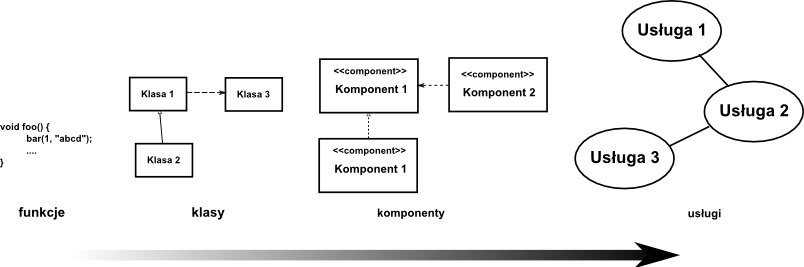
\includegraphics[bb=0 0 386 128]{intro/arch-evo.png}
 \caption{Ewolucja architektur oprogramowania \cite{soa:ibm_soma}}
 \label{fig:soa-ewolucja}
 % arch-evo.png: 427x142 pixel, 94dpi, 11.55x3.84 cm, bb=0 0 327 109
\end{figure}

Rosn�ce wymagania odno�nie mo�liwo�ci, jak i prostoty obs�ugi aplikacji, nieuchronnie prowadz� do wzrostu ich z�o�ono�ci.
Aktualny model tworzenia oprogramowania powoli osi�ga kres swoich mo�liwo�ci
- obserwowany jest znaczny wzrost koszt�w zwi�zanych z rozwi�zywaniem problem�w czysto technologicznych, np. integracj� system�w zbudowanych w oparciu o r�ne platformy po�rednicz�ce (z ang. middleware). In�ynierowie musz� r�wnie� radzi� sobie z ci�g�ymi naciskami organizacyjnymi i biznesowymi takimi jak: ograniczanie koszt�w wytwarzanego oprogramowania, potrzeba szybkiej odpowiedzi na zmieniaj�ce si� wymagania, mo�liwo�� �atwej integracji i absorpcji nowych partner�w biznesowych.
W celu zniwelowania wymienionych trudno�ci powsta�o szereg rozwi�za�, np. architektury przeznaczone do tworzenia system�w rozproszonych, przeno�ne j�zyki programowania, �rodowiska wspieraj�ce integracj� system�w itp.
Nie rozwi�zuj� one jednak wsp�czesnych problem�w - na przeszkodzie staje du�a r�norodno�� platform programistycznych, stosowanych technologii oraz rosn�ca potrzeba integracji system�w.
Brak uniwersalnego i powszechnie stosowanego, a jednocze�nie odpowiadaj�cego obecnym potrzebom rozwi�zania cz�stkowego, przyczyni� si� do powstania koncepcji SOA
- architektury zorientowanej na us�ugi (Service Oriented Architecture). Podstawow� zasad� rz�dz�c� tym podej�ciem jest lu�ne powi�zanie (z ang. loose coupling) pomi�dzy elementami systemu, pozwalaj�ce na proste komponowanie go jako ca�o�ci (zmian� w sposobie projektowania oprogramowania obrazuje \nolinebreak{rysunek \ref{fig:soa-evo2}}).

\begin{figure}[htp]
 \centering
 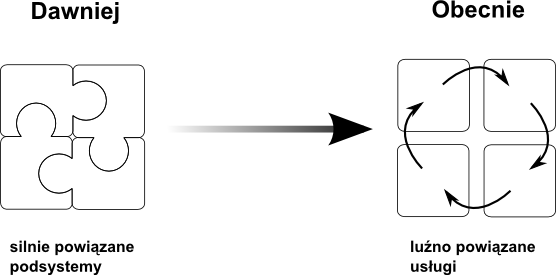
\includegraphics[bb=0 0 267 132]{intro/soa-evolution.png}
 \label{fig:soa-evo2}
 \caption{Zmiana w podej�ciu do projektowaniu oprogramowania}
 % soa-evolution.png: 348x172 pixel, 94dpi, 9.42x4.65 cm, bb=0 0 267 132
\end{figure}

Logiczn� konsekwencj� takiego podej�cia jest zastosowanie szeregu dobrych konwencji in�ynierskich, takich jak ukrycie implementacji\footnote{zwane te� autonomiczno�ci�} czy ponowne u�ycie (z ang. software reuse), przy jednoczesnym wzro�cie elastyczno�ci,  przejrzysto�ci, �atwo�ci wprowadzania zmian oraz prostocie zarz�dzania.

Powszechne uznanie SOA, spowodowa�o zmian� w kierunku rozwoju technologii z zakresu wymiany danych i integracji oprogramowania.
Coraz wi�kszy udzia� w rynku maj� te rozwi�zania, kt�re wi�ksz� uwag� przywi�zuj� do wsp�dzia�ania r�nych platform i przeno�no�ci. Chc�c realizowa� ide� SOA, u�yte technologie musz� dawa� jak najwi�ksz� swobod� w zakresie komunikacji. Ich baz� przestaje by� interfejs programistyczny konkretnego j�zyka, \nolinebreak{a zaczyna} format wymienianych danych. Dodatkowo chc�c zapewni� jak najwi�ksz� niezale�no�� poszczeg�lnych cz�ci system�w, coraz wi�kszy nacisk k�adzie si� na ukrywanie szczeg��w implementacji.

Od czasu opublikowania paradygmatu SOA w 1996 roku, powsta� szereg koncepcji (np. technologia webservice) maj�cych na celu praktyczn� realizacj� SOA.
W oparciu o nie, korzystaj�c jednocze�nie z idei ESB (Enterprise Service Bus) oraz j�zyka BPEL (Business Process Execution Language), firmy informatyczne s� w stanie stworzy� oprogramowanie spe�niaj�ce za�o�enia tej architektury,
obni�aj�ce jednocze�nie koszty rozwoju i utrzymania, jakie nale�a�oby ponie�� przy zastosowaniu tradycyjnego podej�cia.

Budowa oprogramowania w oparciu o technologie realizuj�ce SOA, wi��e si� z narzutami natury wydajno�ciowej. 
% , kt�re mog� by� nieakceptowalne w jego p�niejszym wykorzystaniu.
Jednocze�nie, brak powszechnej wiedzy na temat SOA i utartych dobrych wzorc�w wytwarzania powoduje, �e cz�sto oprogramowanie tworzone w tej architekturze, nie jest napisane w spos�b optymalny, bez wykorzystania jej podstawowych zalet.
Powa�nym wyzwaniem staje si� zatem kwestia pomiaru wydajno�ci tworzonych aplikacji\footnote{Brak zrozumienia kryteri�w wydajno�ciowych jest uznawany za jedno z pi�ciu najwi�kszych zagro�e� SOA \cite{soa:piec_zagrozen}}.

Do tej pory �wiat informatyczny nie dopracowa� si� jednolitej metodologii pomiar�w wydajno�ci system�w o architekturze SOA. Z punktu widzenia in�ynier�w oprogramowania - niemo�liwe jest obecnie przeprowadzenie analizy por�wnawczej takiego oprogramowania.
Istniej�ce rozwi�zania pozwalaj� na pomiary wydajno�ci poszczeg�lnych element�w systemu o architekturze SOA\footnote{Na rynku istnieje szczeg�lnie du�o rozwi�za� do testowania wydajno�ci oprogramowania opartego na technologii webservice}, jednak�e tematyka kompleksowego rozwi�zania tego problemu, nie spotka�a si� dotychczas z du�ym zainteresowaniem, zar�wno ze strony �wiata komercyjnego, jak i naukowego.

\section{Cel pracy}
Celem pracy jest analiza problemu pomiaru wydajno�ci aplikacji zbudowanych w oparciu o paradygmat SOA. Rozwa�onych zostanie kilka potencjalnych rozwi�za� oraz przeanalizowane zostan� zalety i wady ka�dego z nich.
W oparciu o postawiony w pracy zestaw wymaga� zostanie wybrane i zaimplementowane najlepsze.
 % a najlepsze rozwi�zanie zostanie wybrane w oparciu o postawiony w pracy zestaw wymaga�.
Stworzona implementacja zostanie sprawdzona w �rodowisku testowym na zestawie przyk�adowych aplikacji. Proces testowania i wyniki b�d� podstaw� do wyci�gni�cia wniosk�w na temat przydatno�ci wybranego rozwi�zania w analizie wydajno�ci aplikacji opartych o SOA.

\section{Struktura pracy}
Niniejsza praca rozpoczyna si� opisem technologii wykorzystywanych w tworzeniu aplikacji opartych o SOA. W rozdziale 3 szczeg�owo sformu�owano problem oraz zbi�r wymaga� stawianych poszukiwanemu rozwi�zaniu. 
Rozdzia� zawiera ponadto dyskusj� potencjalnych rozwi�za� wraz z ich wadami i zaletami. Wybrane jest jedno, kt�re najlepiej spe�nia postawione wymagania. W rozdziale 4 omawiane s� szczeg�y technologiczne implementacji wybranego rozwi�zania, natomiast w rozdziale 5 wyniki analizy przyk�adowej aplikacji w �rodowisku testowym. Prac� ko�czy rozdzia� 6 zawieraj�cy zbi�r konkluzji odno�nie mo�liwo�ci zastosowania i dalszego rozwoju zaimplementowanego systemu do badania wydajno�ci aplikacji o architekturze SOA.

Rozdzia�y 2.1, 2.2, 3.1, 4, 5.1, 5.5 oraz dodatek A zosta�y napisane przez Tomasza Duszk�. Rozdzia�y 1, 2.3, 2.4, 3.2, 3.3, 3.4, 5.1, 5.2 zosta�y napisane przez Jakuba Janczaka. Pozosta�e rozdzia�y: 6, 7 oraz 8 zosta�y napisane przez autor�w pracy wsp�lnie.
 
%  Rosn�ce nak�ady najwi�kszych gospodarek i �wiatowych koncern�w na systemy komputerowe sprawi�y �e
%  przekroczy�y one swoje naturalne granice. Rozwijaj�cym si� koncernom przesta�o wystarcza� wewn�trzne
%  wspomaganie ich dzia�ania - coraz wi�kszy udzia� w rynku maj� aplikacje zwyczajowo zwane B2B (Business
%  to Business) - maj�ce na celu wymian� informacji pomi�dzy r�nymi podmiotami. Poza tym przemys�, wraz
%  ze wzrostem zaawansowania, rozmiaru i udzia�u oprogramowania zaczyna si� boryka� z problemami jakich
%  wcze�niej nie do�wiadcza�:
% 
% 
% \begin{itemize}
% \item  szybko rozwijaj�cy si� rynek stymuluje powstawanie wielu coraz lepszych i pewniejszych technologii, co w istocie jest pozytywne, ale powoduje i� oprogramowanie ju� napisane bardzo szybko traci na warto�ci i aktualno�ci. Co poza wzrostem wydatk�w mo�e nawet, przy �le prowadzonej polityce doboru, spowodowa� konieczno�� wymiany ca�ych system�w
% \item  silnie zintegrowane systemy wymagaj� ci�g�ej konserwacji, a zmiany w jednej cz�ci zazwyczaj propaguj� si� na pozosta�e 
% \item  coraz wi�ksze skomplikowanie system�w powoduje, i� coraz trudniej je zrozumie� i rozwija�
% \end{itemize}
% 
% \subparagraph{Kr�tki wst�p do SOA}
% 
% SOA (Service Oriented Architecture) to koncepcja kt�rej za�o�enia uwalniaj� oprogramowanie od tych problem�w. SOA promuje model programowania zwany "lu�nym powi�zaniem", tj. komponenty opgramowania s� niezale�nymi bytami (us�ugami), kt�re komunikuj� si� mi�dzy sob� z pomoc� dobrze zdefiniowanych interfesj�w. Us�ugi te wymieniaj� mi�dzy sob� informacje samoistnie lub kierowane przez zewn�trzny proces koordynuj�cy. Praktyka pokaza�a, �e wdro�enie SOA w systemach wielkiej skali przynios�o wiele wymiernych korzy�ci takich jak
% % \footnote{za http://blogs.sun.com/rtenhove/entry/why_soa i http://labs.jboss.com/file-access/default/members/jbossesb/freezone/resources/whitepapers/WhyESB.pdf}:
% 
% \begin{itemize}
% \item  wielokrotne u�ycie komponent�w systemu 
% \item  szybkie reakcje na zmieniaj�ce si� wymagania i realia rynkowe - zmiana w procedurach biznesowych najcz�ciej powoduje zmian� w sposobie wywo�ywania us�ug, a nie ich wewn�trznej implementacji
% \item  mo�liwo�� stosowania przyrostowych metodologii rozwoju oprogramowania - w ostatnim czasie najpopularniejszych w firmach IT, dzi�ki kt�rym mo�liwe jest testowanie cz�sciowej, ju� wykonanej implementacji systemu
% \item  redukcja nak�ad�w poniesionych na oprogramowanie (o czym wspomnieli�my wcze�niej)
% \item  skupienie si� na innowacjach zamiast na konserwacji systemu 
% \end{itemize}
%  Podstaw� powstania SOA jest fakt i� na topie przestaje by� silna integracja, a zaczyna kompozycja :

% img /home/kubek2k/public{\textunderscore}html/dokuwiki/data/media/magisterka/wstep/ewolucja{\textunderscore}soa.png
% 
% 
% 
% \dokutitleleveltree{Problemy z SOA i pr�by rozwi�zania}
% \label{b9e3a44b7fdd9fd1d66bc1fc86f6286e}%% problemy_z_soa_i_proby_rozwiazania
%  Pomimo swoich licznych zalet, podej�cie SOA niesie ze sob� r�wnie� du�a ilo�� problem�w. Chc�c zapewni� wsp�dzia�anie system�w korzystaj�cych z r�nych technologii jeste�my skazani na stosowanie oprogramowania ��cz�cego (z ang. \hyperref[b200f0642a4dc4d9d66162920860c3f0]{middleware}) kt�re jest w je nam w stanie zapewni� - poci�ga to jednak za sob� do�� du�e narzuty czasowe. Zwyczajowo technologi� u�ywan� do integracji system�w w architekurze SOA stosuje si� technologi� \hyperref[742523daef59db4b718409f46de05d0c]{WebService'�w} opartych o protok� \hyperref[cbf4e0b7971051760907c327e975f4e5]{SOAP}. Dodatkowo wykorzystanie samej architektury SOA nak�ada na tworz�cych konieczno�� zaszywania lokalizacji poszczeg�lnych komponent�w systemu (tj. ka�da z us�ug musi wiedzie� gdzie powinna skierowa� kolejne ��dania, w zale�no�ci od otrzymanych danych).
% 
% 
% \dokutitlelevelfour{BPEL}
% Chc�c zmieni� naturalne podej�cie do wykonywania ci�gu operacji na rozproszonych us�ugach (tzw. choreografii), wprowadzono poj�cie orchiestracji. \hyperref[54f21b6ecfc3292b6bcc669edc745133]{Orchiestracja} polega na tym, �e z komponent�w systemu spada konieczno�ci bycia �wiadomym o otoczeniu - wprowadzone zostaje poj�cie procesu biznesowego kt�ry sam wie co ma robi� z danymi, i zawiaduje sekwencjami wywo�a�. Zmian� podej�cia mo�na por�wna� do przej�cia z modelu \hyperref[705bcf0e77bc8b6fc8e66cbf3c055e6c]{peer-to-peer} do modelu scentralizowanego.
% 
% Jednym z rozwi�za� wspieraj�cych ide� orchiestracji jest j�zyk BPEL - Business Process Execution Language. Dzi�ki niemu jeste�my w stanie modelowa� nawet bardzo z�o�one procesy biznesowe na r�nych stopniach abstrakcji, korzystaj�c ze standardowych element�w sk�adniowych znanych z innych j�zyk�w programowania. Co najwa�niejsze zosta� on pomy�lany w taki spos�b, aby modele da�o si� przedstawi� w postaci graficznej - bloczk�w, dzi�ki czemu proces tworzenia aplikacji ulega bardzo znacznemu uproszczeniu, a zarazem powi�ksza si� grono potencjalnych u�ytkownik�w. Nie bez znaczenia jest r�wnie� obecno�� du�ej gamy narz�dzi do modelowania w BPEL.
% 
% Co wa�ne standard ten jest bardzo silnie wspierany przez przemys� informatycznym i bez w�tpienia b�dzie w najbli�szym czasie b�dzie to jedyny sensowny wyb�r na tym polu. Liczby \dokufootnote{ankieta OASIS: \href{http://mult.ifario.us/p/bpel-adoption-thermometer}{http://mult.ifario.us/p/bpel-adoption-thermometer}} pokazuj�, i� w�r�d programist�w tworz�cych systemy SOA 23\% korzysta, a 28 planuje u�ywa� BPEL w swoich aplikacjach \dokufootnote{z drugiej strony 40\% nadal nie wie co to BPEL, co pokazuje nam jak niedojrza�y jest jeszcze ten rynek}. Liczby te rosn� z roku na rok. \dokufootnote{wi�cej informacji o BPEL \hyperref[22ee86570f52c823bdb1d5ef39aed4f7]{tutaj}}
% 
% 
% \dokutitlelevelfour{ESB}
% Innym, wspomnianym wcze�niej, problemem jest mnogo�� u�ywanych technologii w zewn�trznych i ju� istniej�cych systemach (tzw. systemach odziedziczonych). Cz�sto okazuje si�, �e pomimo najwi�kszych stara� nie jest mo�liwe dostosowanie si� do takowych, a architektura SOA oparta tylko i wy��cznie na \hyperref[742523daef59db4b718409f46de05d0c]{Web Service'ach} zaczyna traci� na swoich w�asno�ciach. Rozwi�zania mog� by� dwa:
% 
% 
% \begin{itemize}
% \dokuitem  prostsze - mo�na stworzy� opgramowanie opakowuj�ce (tzw. wrapper) dla danej us�ugi, zrzucaj�c na siebie tym samym konieczno�� zmian za ka�dym razem kiedy ta us�uga zmieni si�
% \end{itemize}
% lub
% 
% 
% \begin{itemize}
% \dokuitem  bardziej z�o�one, ale daj�ce wi�kszy zysk w przysz�o�ci - mo�na u�y� istniej�cych platform integracyjnych (tzw. "integration middleware")
% \end{itemize}
% \hyperref[efb03b68f7a0c2a331fc61a491c4b2d7]{ESB (Enterprise Service Bus)} jest w�a�nie jedn� z takich platform. Jej idea opiera si� na istnieniu szyny danych przy pomocy kt�rej realizujemy wszystkie komunikacje w systemie. Dzi�ki temu to nie proces, a szyna mo�e decydowa� o tym gdzie ma trafi� dana informacja. Takie dzia�anie daje bardzo du�e mo�liwo�ci, szczeg�lnie je�li chodzi o przeno�no�� poniewa� chc�c skorzysta� z jakiej� us�ugi proces nie odwo�uje si� do konkretnej instancji, ale po prostu wysy�a odpowiednio spreparowan� wiadomo�� do szyny i oczekuje na odpowied�. Dzi�ki takiem podej�ciu znacznie prostsze staje si� zapewnienie wielu wa�nych w�a�ciwo�ci systemu rozproszonego:
% 
% 
% \begin{itemize}
% \dokuitem  integracja z innymi technologiami - ujednolicenie "punktu styku" ze �rodowiskiem zewn�trznym i istniej�cymi systemami, za pomoc� odpowiednich adapter�w i konwerter�w wiadomo�ci
% \dokuitem  rozwi�zanie problemu lokalizacji us�ug - to szyna decyduje gdzie wys�a� dan� wiadomo��  zatem nasze aplikacje staj� si� przeno�ne, wszystko zale�y od konfiguracji ESB
% \dokuitem  dzi�ki zastosowaniu redundantnych us�ug i odpowiedniej konfiguracji jeste�my wstanie zapewni� wy�sz� wydajno�� i niezawodno�� systemu
% \dokuitem  dzieki temu, �e dane pod��aj� niejako jednym kana�em komunikacyjnym �atwiejsze staje si� zarz�dzanie bezpiecze�stwem 
% \end{itemize}
%  Mimo swojej kr�tkiej historii koncepcja ESB udowodni�a ju� swoj� przydatno�� w budowaniu du�ych system�w. ESB jest z powodzeniem wdra�ane w wielu inicjatywach ze szczeg�lnym uwzgl�dnieniem du�ych projekt�w rz�dowych \dokufootnote{np. \href{http://www.gcn.com/print/25_20/41319-1.html}{system dla policji stanu Washington} czy \href{http://newsroom.progress.com/phoenix.zhtml?c=86919&p=NewsArticle&id=997931}{systemy bukmacherskie w UK}} \dokufootnote{wi�cej informacji o ESB \hyperref[efb03b68f7a0c2a331fc61a491c4b2d7]{tutaj}}
% 
% 
% \dokutitleleveltree{Podsumowanie}
% \label{96e21bf66c0133beafda0ff9f011643e}%% podsumowanie
% Jak wida� rynek informatyczny poradzi� sobie z g��wnymi problemami z kt�rymi spotyka si� programista stosuj�cy architektur� SOA. Jednak otaczaj�c ju� w samym sobie "ci�k�" technologi� \hyperref[742523daef59db4b718409f46de05d0c]{WebService'�w} dodatkowymi rozwi�zaniami, ryzykujemy sytuacj� w kt�rej to ich narzut b�dzie mia� bardzo znacz�cy udzia� w wykonaniu tych operacji. Dodatkowo zagro�eniem dla tych technologii jest (sic!) ich dynamiczny rozw�j w ostatnich latach\dokufootnote{co tyczy si� w zasadzie ca�ego rynku oprogramowania na �wiecie} - istnieje zagro�enie, �e producenci oprogramowania popychani coraz wi�ksz� konkurencj� na rynku, k�ad� wi�kszy nacisk na mo�liwo�ci pomijaj�c tak istotne cechy jak odporno�� na b��dy czy wydajno��. 
% 
% Chc�c por�wna� dzia�anie r�nych rozwi�za�, tudzie� sprawdzi� narzut wynikaj�cy z wdro�enia danej technologii, musi istnie� jaka� sp�jna metodologia pomiar�w wydajno�ci - kt�rej rynek do tej pory niedopracowa� si�. 
% 
% Celem tej pracy jest pokazanie jakie podej�cie nale�y zastosowa� do pomiar�w wydajno�ci system�w o architekturze SOA. Efektem pracy ma by� r�wnie� stworzenie narz�dzia do takich pomiar�w, oraz opracowanie przyk�adowych wynik�w test�w w oparciu o przyk�adow� aplikacj� stworzon� w oparciu o wymienione wcze�niej technologie.
% 
% 
% \dokutitleleveltwo{Koniec}
% \label{44943fe207611d5625258c1059d25ec8}%% koniec
% Napisa� o mo�liwym narzucie generowanym przy takiej ilo�ci technologii i konieczno�ci pomiar�w.
% 
%  Chc�c omin�� problemy z integracj� system�w stworzonych z u�yciem r�nych technologii i operuj�cych w r�nego rodzaju �rodowiskach, jako standard w zastosowaniach architektury SOA przyj�o si� stosowa� technologi� \hyperref[cca5d72b2013a1b8737449a4dd328903]{WebSevice'�w}. U�ycie tak "ci�kiego" podej�cia do zdalnego korzystania z us�ug ma jednak bardzo du�e prze�o�enie na wydajno�� aplikacji. Z tego powodu istotnie wa�nym staje si� fakt i� brak jest zunifikowanego podej�cia do badania jak wydajne s� aplikacje spe�niaj�ce za�o�enia SOA. Taki stan rzeczy dodatkowo daje argument tzw. SOA-sceptykom, kt�rzy jako g��wn� wad� tej architektury wymieniaj� w�a�nie straty wydajno�ciowe. 
% 
% Celem tej pracy b�dzie opracowanie takiego podej�cia ze szczeg�lnym uwzgl�dnieniem aplikacji opracowanych w oparciu o BPEL\ldots{}. i nie wiem co tu dalej napisac ;)
% 
% "My thought was, this change has to be compared to the switsch from Newtonian physics to relativistic physics." - \href{http://weblogs.asp.net/ralfw/archive/2005/07/03/417507.aspx}{http://weblogs.asp.net/ralfw/archive/2005/07/03/417507.aspx}
% 
% Melted Cheese programming - przej�cie z SOA - \href{http://msdn2.microsoft.com/en-us/library/ms954609.aspx}{http://msdn2.microsoft.com/en-us/library/ms954609.aspx}
% 
% [mniej patetycznie, wi�cej konkret�w, gar�� fakt�w]
% 
%  Dodatkowym problem, kt�ry jest szczeg�lnie istotny w obecnych czasach, to du�a pr�dko�� rozwoju przemys�u i technologii informatycznych. Cz�sto okazuje si� �e technologia traci swoj� warto�ci na przestrzeni miesi�cy.  



\chapter{Technologie}

W rozdziale tym zaprezentowano przegl�d najwa�nieszych technologii u�ywanych do realizacji paradygmatu SOA.

\section{SOA}

Zwi�kszone zainteresowanie SOA zwi�zane jest z rozpowszechnianiem si� technologii webservice i dyskusjami na temat zysk�w, kt�re mo�na dzi�ki ich wdro�eniu osi�gn��. Problemy poruszane w tych dyskusjach nie s� nowe, pojawia�y si� ju� od czasu gdy technologia CORBA umo�liwi�a integracj� heterogenicznych aplikacji z r�nych �rodowisk. Do problem�w tych - zwi�zanych z integracj� aplikacji - mo�na zaliczy� np:

\begin{itemize}
 \item niezgodno�� danych na poziomie binarnym (np. jeden komputer u�ywa kodowania Big Endian a inny Little Endian)
 \item konieczno�� obs�ugi rozproszonych mechanizm�w transakcyjnych, autoryzacji i uwierzytelniania
 \item r�nice koncepcyjne pomi�dzy u�ytymi platformami po�rednicz�cymi (np. RMI operuje na poziomie wywo�ania metody interfejsu, Sun RPC na poziomie wywo�ania funkcji)
\end{itemize}

Technologie obiektowe stworzone w latach 90 XX wieku (CORBA, DCOM, RMI itp.) pozwalaj� na integracj� aplikacji oraz zmniejszaj� konieczno�� nadmiernego skupiania si� in�ynier�w nad kwestiami technologicznymi tego procesu. Dla przyk�adu obiekty w technologii CORBA (wykorzystuj�cej do transportu protok� IIOP) mog� komunikowa� si� nie tylko z innymi obiektami CORBA, ale tak�e np. z RMI. Technologie te nie rozwi�za�y wszystkich problem�w integracyjnych, a opr�cz nich zacz�y pojawia� si� nowe utrudnienia:

\begin{itemize}
 \item statyczno�� obiekt�w, brak mo�liwo�ci wymiany wadliwych w trakcie dzia�ania systemu
 \item �cis�e powi�zanie element�w systemu (z ang. tight coupling)
 \item redundantno�� oprogramowania (np. implementacja tej samej funkcjonalno�ci w kilku systemach)
 \item brak ponownego u�ytkowania ju� stworzonych podsystem�w
 \item integracja N podsystem�w (z kt�rych ka�dy mo�e u�ywa� ka�dego innego) wymaga�a ilo�ci po��cze� proporcjonalnej do kwadratu ilo�ci podsystem�w (por. rysunek \ref{fig:integr})
\end{itemize}

\begin{figure}[h!]
 \centering
 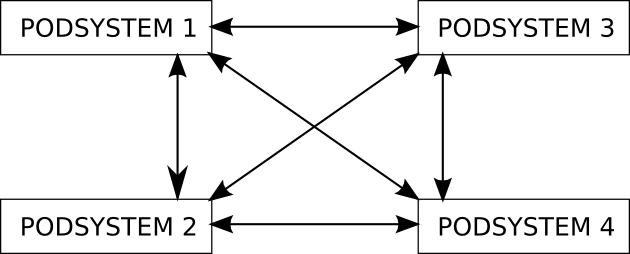
\includegraphics[bb=0 0 241 97]{chapter1/integr.png}
 % integr.png: 631x254 pixel, 188dpi, 8.51x3.43 cm, bb=0 0 241 97
 \caption{Schemat integracji 4 podsystem�w (ka�dy-z-ka�dym)}
 \label{fig:integr}
\end{figure}


Na prze�omie XX i XXI wieku pojawi�y si� technologie, kt�rych u�ycie pozwoli�o rozwi�za� cz�� wspomnianych problem�w.
Najpopularniejsze z nich to technologia webservice. Jednak opr�cz technologii potrzebny by� r�wnie� og�lny opis architektury. Architektury, w kt�rej aplikacje mog�y by� tworzone, integrowane i powt�rnie u�ytkowane; kt�ra umo�liwi�aby sk�adanie aplikacji z gotowych element�w w celu szybkiego dostarczania rozwi�za�. Pr�b� odpowiedzi na te potrzeby by�o zaproponowanie SOA.

\begin{quotation}
 \textbf{SOA} (\textbf{Service Oriented Architecture}) \cite{soa:open_group_def} - architektura zorientowana na lu�no powi�zane \textbf{us�ugi}.
\end{quotation}

\begin{quotation}
 \textbf{Us�uga} - logiczna reprezentacja powtarzalnej czynno�ci biznesowej maj�ca oczekiwany rezultat (np. pobierz prognoz� pogody, sprawd� czy osoba figuruje w krajowym rejestrze d�ug�w)\cite{soa:open_group_def}.
\end{quotation}

Podkre�lenia wymaga fakt, �e SOA i webservice nie s� poj�ciami r�wnoznacznymi. Us�ugi webservice s� dowodem i przyk�adem na istnienie technologii, kt�ra umo�liwia konstrukcj� systemu zgodnego z SOA. 
% Zostan� om�wione bardziej szczeg�owo w nast�pnym rozdziale.

Na rysunku \ref{fig:soa} znajduje si� przyk�adowy schemat funkcjonowania aplikacji opartej o SOA. Pierwszym etapem jej dzia�ania jest wyszukanie wymaganej us�ugi w rejestrze (uzyskuje si� w ten spos�b m.in. informacj� o lokalizacji us�ugi). Nast�pnie do us�ugi wys�ane zostaje ��danie wykonania operacji, kt�re jest przez ni� przetwarzane a rezultat odes�any z powrotem do aplikacji. Schemat ten jest powielany dla ka�dej z us�ug, a ca�y ci�g wywo�a� jest sterowany kodem aplikacji SOA.

\begin{figure}[h!]
 \centering
 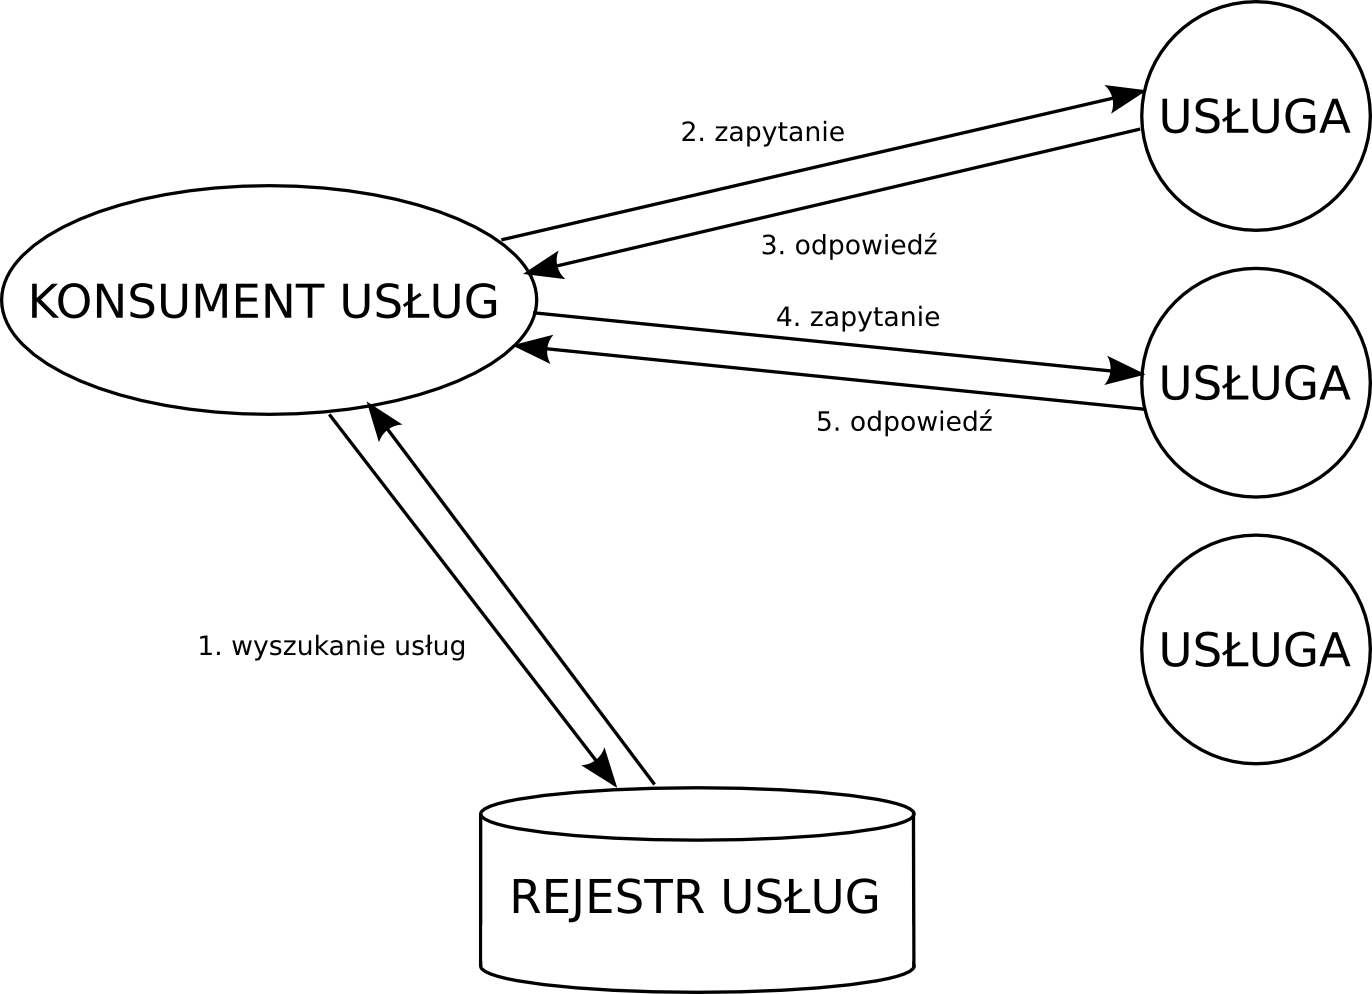
\includegraphics[bb=0 0 330 238]{chapter1/soa.png}
 % soa.png: 412x298 pixel, 90dpi, 11.63x8.41 cm, bb=0 0 330 238
 \caption{Przyk�adowy schemat funkcjonowania aplikacji opartej o SOA}
 \label{fig:soa}
\end{figure}

\subsection{Kluczowe elementy}

Wybrane elementy funkcjonowania systemu opartego o SOA:
\begin{enumerate}
 \item Wszystkie operacje systemu s� zdefiniowane jako \textbf{us�ugi}. Mog� to by� zar�wno proste operacje biznesowe (pobierz stan konta), operacje transakcyjne zbudowane z innych us�ug (przelew mi�dzy rachunkami) jak i funkcje systemowe (np. wy�lij e-mail). Do in�ynier�w nale�y decyzja o poziomie ziarnisto�ci oferowanych us�ug.
 \item Interfejs us�ugi jest \textbf{odseparowany} od implementacji. Konsumenci us�ugi nie znaj� dok�adnego sposobu realizacji operacji, znaj� jedynie semantyk� i syntaktyk� tej operacji.
 \item Prawid�owe funkcjonowanie systemu przy zachowaniu lu�nego wi�zania (ang. loose coupling) mi�dzy us�ugami uzyskuje si� dzi�ki wprowadzeniu \textbf{kontrakt�w}.
 \item System jest \textbf{systemem dynamicznym}. W trakcie jego dzia�ania mo�na dodawa� nowe us�ugi oraz wymienia� stare (np. poprawia� znalezione w nich b��dy, konstruowa� efektywniejsze wersje us�ugi).
 \item Istnieje mo�liwo�� \textbf{wielokrotnej implementacji} tej samej us�ugi w r�nych wersjach (np. za pomoc� r�nych algorytm�w, r�nych dostawc�w). U�ytkownik decyduje kt�rej instancji us�ugi chce u�y� (np. tej kt�ra w danej chwili jest najmniej obci��ona lub tej kt�ra jest najta�sza).
 \item Budowanie systemu odbywa si� na zasadzie \textbf{kompozycji} z istniej�cych ju� us�ug. Poprzednio systemy by�y tworzone poprzez integracj� element�w, co powodowa�o konieczno�� pisania kodu dostosowuj�cego mechanizmy tych element�w (np. sposobu komunikacji, obs�ugi transakcji, kontroli dost�pu).
 \item Wyst�puje ca�kowita \textbf{transparentno�� lokalizacji}. Konsument us�ugi nie jest �wiadomy gdzie fizycznie operacje danej us�ugi s� wykonywane. Us�uga mo�e w spos�b niezauwa�alny dla konsumenta migrowa� pomi�dzy maszynami w trakcie dzia�ania systemu albo by� zreplikowana na kilka maszyn w celu zmniejszenia czasu wykonywania operacji.
\end{enumerate}
Dodatkowej uwagi wymaga poj�cie kontrakt�w, b�d�cych podstaw� prawid�owej konstrukcji oprogramowania opartego o SOA.

\subsection{Kontrakt}

Kontrakty s� zawierane ka�dorazowo pomi�dzy us�ug� a jej konsumentem (kt�rym mo�e by� tak�e inna us�uga). Umo�liwiaj� separacj� interfejs�w od implementacji oraz realizacj� lu�nych powi�za� pomi�dzy us�ugami (modyfikacja szczeg��w implementacji us�ugi nie powoduje zmian w kontrakcie, a wi�c jest transparentna dla konsument�w danej us�ugi). Zawieraj� opis informacji oferowanych i oczekiwanych przez us�ug�. Dobry kontrakt powinien zawiera� nast�puj�ce pozycje \cite{soa:kontrakt}:

\begin{itemize}
 \item og�lne informacje o us�udze
   \begin{itemize}
    \item nazwa kontraktu, wersja
    \item w�a�ciciel (osoba/organizacja)
    \item rodzaj us�ugi (np. integracyjna, prezentacyjna, biznesowa)
   \end{itemize}
 \item opis funkcjonalny operacji zawartych w us�udze
   \begin{itemize}
    \item semantyka operacji (wymagania funkcjonalne w stosunku do us�ugi)
    \item syntaktyka operacji (typy argument�w i rezultat�w, wyj�tki)
    \item szczeg�y sposobu wywo�ania operacji (adres URL us�ugi oraz rodzaj protoko�u transportu np. SOAP)
   \end{itemize}
 \item opis niefunkcjonalny
   \begin{itemize}
    \item transakcyjno�� operacji
    \item QoS (Quality of Service)
    \item SLA (Service Level Agreement) np. dozwolone op�nienie w wykonywaniu us�ugi
    \item autoryzacja, ograniczenie dost�pu do operacji serwisu okre�lonej grupie konsument�w
   \end{itemize}
\end{itemize}

Podkre�lenia wymaga fakt, �e nie istnieje sformalizowana posta� kontraktu SOA. Powy�sze informacje s� jedynie proponowan� zawarto�ci� kontraktu. Rzeczywista zawarto�� kontraktu b�dzie mia�a r�n� posta� w zale�no�ci od u�ytej technologii.



\bigskip
Paradygmat SOA w praktyce mo�e zosta� zrealizowany na r�ne sposoby. Najpopularniejszym z nich jest u�ycie technologii webservice.
\section{Webservice}

Mi�dzynarodowa organizacja W3C \cite{misc:w3c} zajmuj�ca si� ustanawianiem standard�w dotycz�cych Internetu zdefiniowa�a webservice w spos�b nast�puj�cy\cite{ws:w3c_def}:

\begin{quotation}
 \textbf{Webservice} - oprogramowanie wspieraj�ce wymian� danych mi�dzy maszynami poprzez sie�, wykorzystuj�ce w tym celu zbi�r ustandaryzowanych technologii (WSDL, XML, SOAP, UDDI)\cite{ws:w3c_def}.
\end{quotation}

Webservice nie jest synonimem SOA. SOA jest to architektura zorientowana na lu�no powi�zane us�ugi, podczas gdy webservice jest to zbi�r konkretnych technologii (WSDL, XML, SOAP, UDDI), u�ytych do realizacji SOA. Technologia webservice jest wi�c przyk�adowym sposobem realizacji SOA, nie jedynym, ale w dotychczasowej praktyce jednym z najpopularniejszych.

Przyk�adowy scenariusz u�ycia webservice zaprezentowany zosta� na rysunku \ref{fig:soa-ws}. Sk�ada si� on z nast�puj�cych etap�w:
\begin{itemize}
 \item wyszukanie konkretnej us�ugi w rejestrze UDDI
 \item uzyskanie dokumentu WSDL us�ugi
 \item wys�anie zapytania zgodnego z protoko�em SOAP do us�ugi
 \item przetworzenie zapytania przez us�ug�
 \item odebranie odpowiedzi zgodnej z protoko�em SOAP od us�ugi
\end{itemize}

% przyk�ad us�ug webservice z zaznaczonymi WSDL, XML, SOAP, UDDI
\begin{figure}[h!]
 \centering
 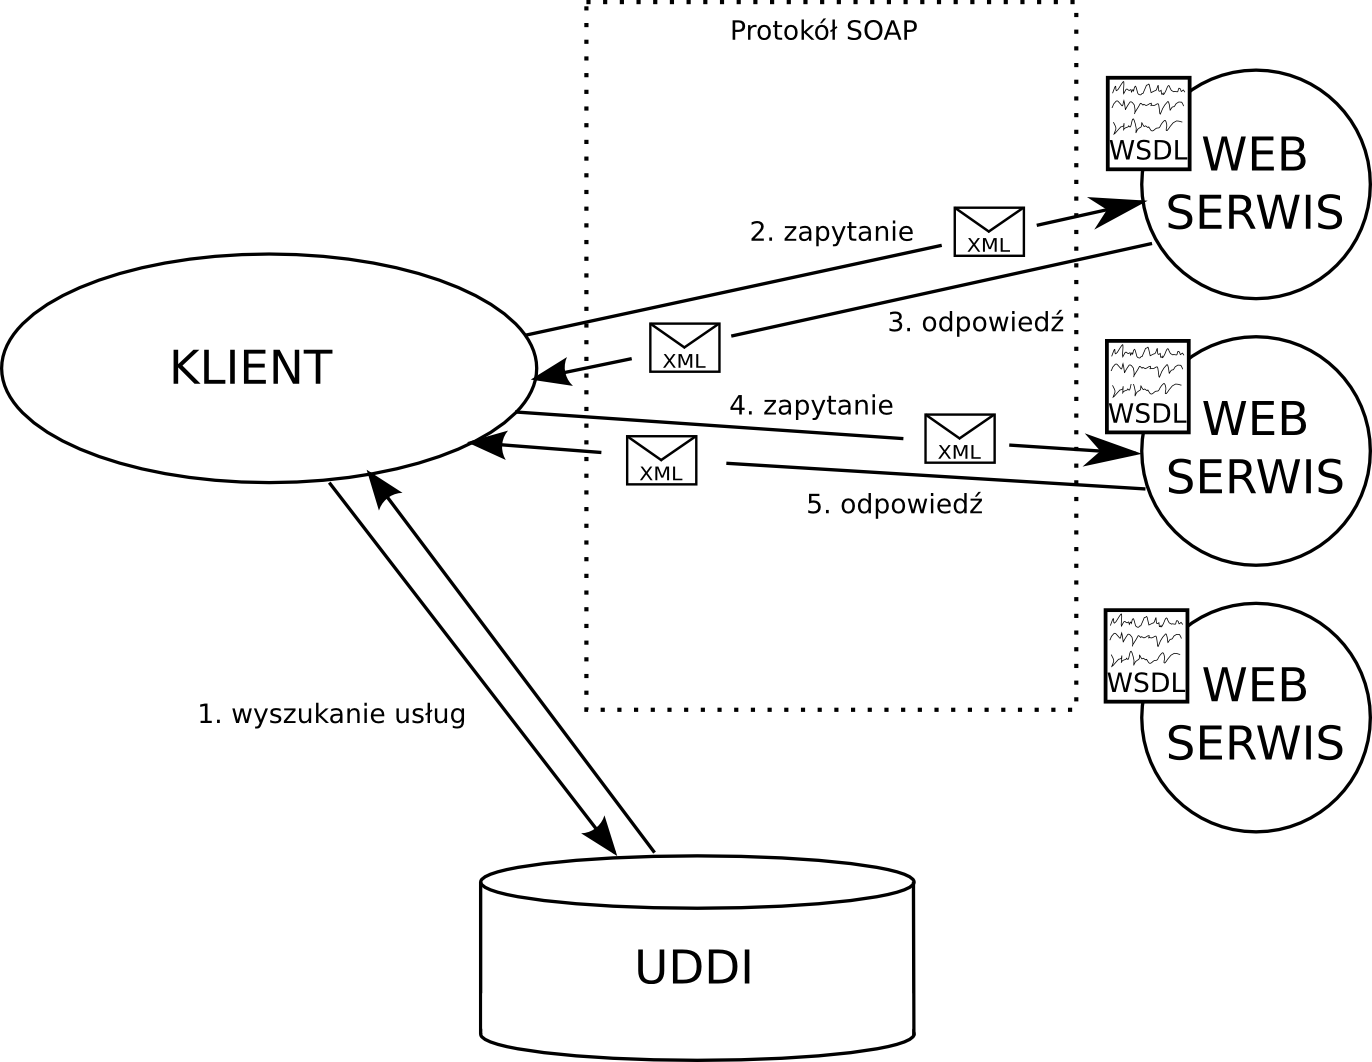
\includegraphics[bb=0 0 330 255]{chapter1/soa-ws.png}
 % soa-ws.png: 412x319 pixel, 90dpi, 11.63x9.00 cm, bb=0 0 330 255
 \caption{Przyk�ad funkcjonowania aplikacji opartej o us�ugi webservice}
 \label{fig:soa-ws}
\end{figure}

Implementacja us�ug webservice odbywa si� z wykorzystaniem ustandaryzowanych technologii:
\begin{itemize}
 \item WSDL (Web Service Definition Language) - opis us�ugi w postaci XML
 \item SOAP - protok� wymiany danych z us�ugami
 \item UDDI (Universal Description, Discovery and Integration) - obs�uga rejestru us�ug.
\end{itemize}

\subsection{WSDL}

WSDL (Web Service Definition Language) jest to dokument XML opisuj�cy webservice. Mo�e przechowywa� zar�wno og�ln� informacj� o us�udze (operacje i ich argumenty) jak r�wnie� szczeg�owe informacje (powi�zanie us�ug z protoko�ami i adresami pod kt�rymi us�ugi te s� dost�pne). Plik WSDL sk�ada si� z definicji nast�puj�cych element�w (w nawiasach podano oryginalne angielskie nazwy)\cite{ws:wsdl:spec}:
\begin{itemize}
 \item typ (type) - definicja typu danych
 \item komunikat (message) - z�o�ony typ danych
 \item operacja (operation) - definicja operacji wraz z komunikatami zawieraj�cymi argumenty oraz rezultat operacji
 \item typ portu (port type) - zbi�r operacji
 \item wi�zanie (binding) - typ portu powi�zany z konkretnym protoko�em (np. SOAP+HTTP)
 \item port (port) - wi�zanie wraz z adresem (np. URL dla HTTP, e-mail dla SMTP)
 \item us�uga (service)- zbi�r port�w
\end{itemize}

Dokument WSDL nie jest obowi�zkowym elementem ka�dego webservice. Je�li jednak wyst�puje to jest on realizacj� kontraktu SOA pomi�dzy us�ug� a jej konsumentem. Zawiera opis parametr�w oczekiwanych przez us�ug� oraz oferowanych (typ rezultatu, nazwy operacji okre�laj�ce ich semantyk�). Nie odwo�uje si� w �aden spos�b do implementacji us�ugi, dzi�ki czemu wyst�puje separacja pomi�dzy interfejsem us�ugi (opisywanym w WSDL i kontrakcie) a jej implementacj�. Zmiany w implementacji us�ugi - nie powoduj�ce zmian w semantyce ani syntaktyce operacji - nie zmieniaj� dokumentu WSDL tej us�ugi. Tym samym nie naruszaj� kontraktu i nie wymagaj� zmian u konsument�w us�ugi.

\subsection{SOAP}

SOAP (dawniej Simple Object Access Protocol, p�niej Service Oriented Architecture Protocol, obecnie brak oficjalnego rozwini�cia tego akronimu\cite{ws:w3c_soap}) jest to protok� opisuj�cy spos�b kodowania i wymiany wiadomo�ci w formacie XML. Do przesy�ania wiadomo�ci zakodowanej zgodnie z SOAP najcz�ciej wykorzystuje si� protok� HTTP/HTTPS (ze wzgl�du na jego popularno�� w internecie), ale mo�liwe jest te� wykorzystanie np. SMTP, FTP, RMI/IIOP. Protok� SOAP mo�e by� u�yty w realizacji r�nych wzorc�w wymiany wiadomo�ci (MEP - Message Exchange Pattern), ale dla potrzeb webservice u�ywa si� go w RPC (RPC - Remote Procedure Call)\cite{ws:w3c_soap_rpc}.

Wiadomo�� SOAP z za��cznikami sk�ada si� z:
\begin{itemize}
 \item w�a�ciwej wiadomo�ci SOAP w formacie XML
  \begin{itemize}
   \item element�w nag��wka (opcjonalne)
   \item tre�ci wiadomo�ci
  \end{itemize}
 \item za��cznik�w przechowuj�cych dane binarne
\end{itemize}

\begin{figure}[h!]
 \centering
 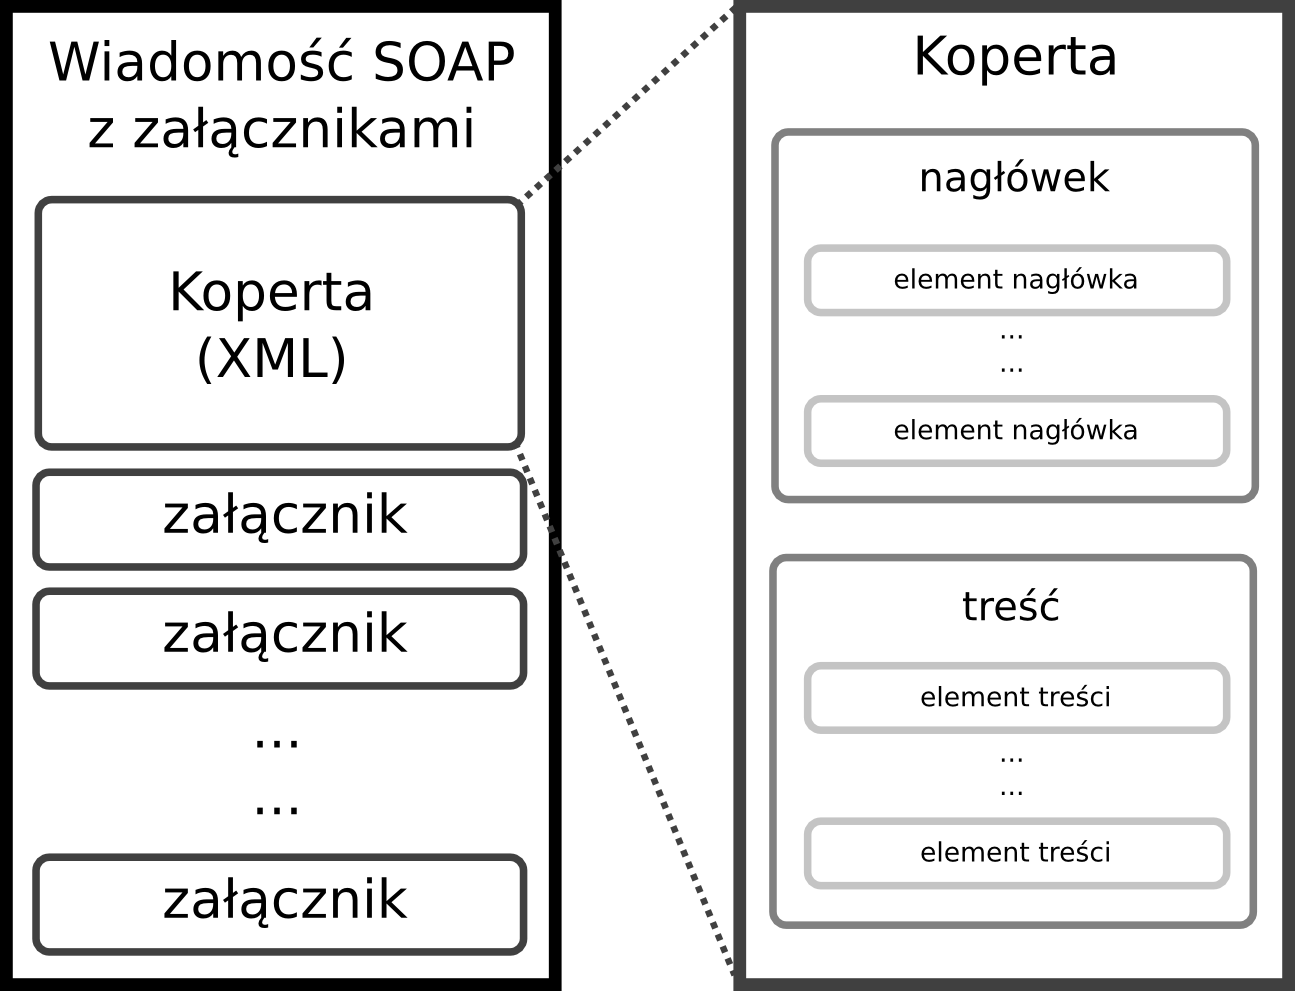
\includegraphics[bb=0 0 311 238]{chapter1/soap.png}
 % soap.png: 1295x991 pixel, 300dpi, 10.96x8.39 cm, bb=0 0 311 238
 \caption{Posta� wiadomo�ci SOAP z za��cznikami \cite{ws:suntechdays}}
 \label{fig:soap}
\end{figure}

Proces wykonania operacji danego webservice rozpoczyna si� od stworzenia odpowiedniej wiadomo�ci w formacie SOAP. Format tej wiadomo�ci zosta� przedstawiony na rysunku \ref{fig:soap}. W jej tre�ci przesy�ane s� informacje o ��danej operacji oraz warto�ciach jej parametr�w. Dodatkowo (w nag��wku) mog� by� przekazane np. parametry do autoryzacji (nazwa u�ytkownika i has�o), identyfikator sesji. Po wys�aniu wiadomo�ci do us�ugi (np. na adres uzyskany z pliku WSDL) nast�puje wykonanie ��danej operacji i odes�anie odpowiedzi do nadawcy. Odpowied� jest r�wnie� zakodowana w formacie SOAP i zawiera informacje o rezultacie wykonania operacji (lub ewentualnych wyj�tkach).

\subsection{UDDI}
UDDI (Universal Description, Discovery and Integration)\cite{ws:uddi} - technologia pozwalaj�ca na publikacj� i wyszukiwanie informacji o us�ugach webservice. Jest to otwarty standard zarz�dzany przez organizacj� OASIS \cite{ws:oasis}. Spos�b wykorzystania UDDI opiera si� na mechanizmie publikacja-wyszukanie-powi�zanie (z ang. publish-find-bind) przedstawionym na \nolinebreak{rysunku \ref{fig:uddi}}:
\begin{itemize}
 \item u�ycie us�ugi musi by� poprzedzone \textbf{opublikowaniem} jej w rejestrze
 \item konsument \textbf{wyszukuje} interesuj�ce go us�ugi w rejestrze
 \item po znalezieniu us�ugi nast�puje \textbf{powi�zanie} jej z konsumentem, kt�ry uzyskuje mo�liwo�� wykonywania operacji tej us�ugi
\end{itemize}


\begin{figure}[h!]
 \centering
 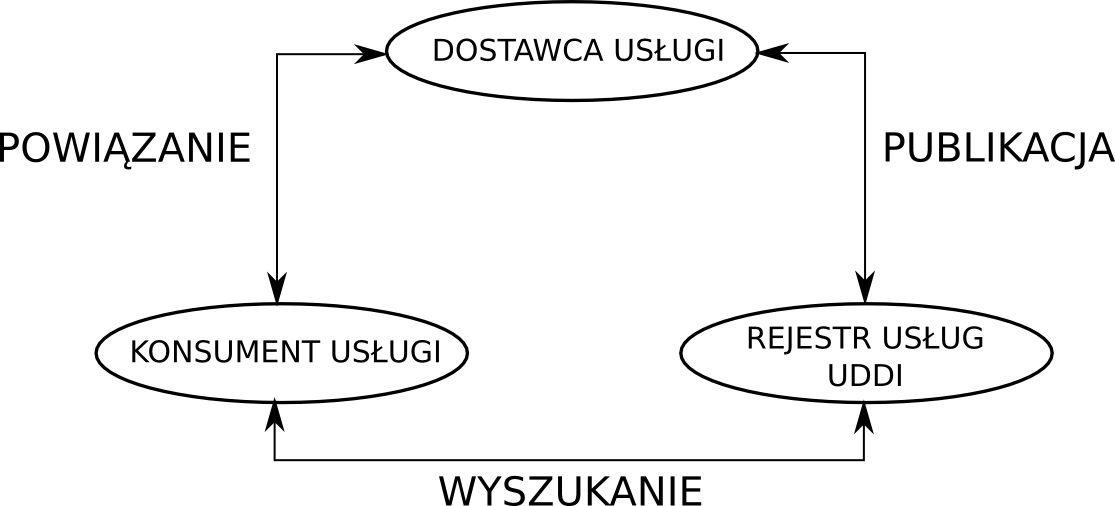
\includegraphics[bb=0 0 268 122]{chapter1/uddi.png}
 % uddi.png: 700x318 pixel, 188dpi, 9.44x4.29 cm, ABB=0 0 268 122
 \caption{Schemat wykorzystania UDDI \cite{ws:suntechdays}}
 \label{fig:uddi}
\end{figure}

UDDI przechowuje informacj� o zbiorze podmiot�w biznesowych. Pojedy�czy wpis o podmiocie biznesowym podzielony jest na nast�puj�ce grupy:
\begin{itemize}
 \item ``white pages'' - adres, dane kontaktowe
 \item ``yellow pages'' - kategorie do jakich nale�y biznes i jego us�ugi
 \item ``green pages'' - techniczne informacje o udost�pnianych us�ugach (m.in. adresy URL plik�w WSDL)
\end{itemize}

W roku 2000 wraz ze specyfikacj� standardu UDDI powsta� publiczny rejestr us�ug UDDI stworzony przez firm� IBM, Microsoft oraz SAP \cite{ws:uddi:public}. 
%Rejestr ten zosta� wy��czony w roku 2006 i do tego czasu 
W rejestrze tym, do momentu jego wy��czenia w roku 2006, zgromadzono ponad 50000 wpis�w o us�ugach \cite{ws:uddi:public}. Wy��czenie publicznego rejestru by�o efektem zwi�kszaj�cego si� zainteresowania podmiot�w biznesowych prywatnymi rejestrami UDDI.


\bigskip
Opr�cz technologii webservice mo�liwo�� realizacji paradygmatu SOA daje r�wnie� platforma integracyjna ESB.
\section[ESB]{Enterprise Service Bus}

% 
ESB (Enterprise Service Bus) to jedno z podej�� kt�re u�atwia tworzenie oprogramowania o architekturze SOA. Zak�ada ono tworzenie sterowanego zdarzeniami systemu opartego o lu�no powi�zane us�ugi. Wymiana danych jest dokonywana przez szyn�,
 kt�rej zadaniem jest wyznaczanie tras wiadomo�ci, na podstawie dostarczonej konfiguracji. G��wnym zamiarem jej tw�rc�w by�o rozlu�nienie powi�zania pomi�dzy wykorzystywanymi us�ugami, a medium transportowym, co przedstawia rysunek \ref{fig:esb}. 
 
% Jest to oparta na standardach platforma integracyjna, kt�ra
% ��czy w sobie zalety takich podej�� jak komunikacja w oparciu o wiadomo�ci, technologia WebService, transformacje danych, inteligentne wyznaczanie trasy, niezawodno��, orchiestracja i transakcyjno�� w komunikacji pomi�dzy r�norodnymi
% aplikacjami korporacyjnymi\footnote{z ang. \textit{enterprise applications}}.
% Ca�a idea opiera si� na istnieniu szyny, w oparciu o kt�r� odbywa si� ka�da komunikacja w obr�bie tworzonego systemu. Odpowiednio skonfigurowana - jest w stanie sama decydowa� o przeznaczeniu ka�dej wiadomo�ci, na podstawie jej tre�ci\footnote{z ang. content based routing}.
% Skonfigurowana szyna decyduje o tym gdzie ma zosta� wys�ana przetwarzana wiadomo��.
% Dzi�ki swoim w�a�ciwo�ciom szyna jest w stanie sama
% decydowa� o tym gdzie ma wys�a� dan� wiadomo��. % napisa� o tym �e to my decydujemy o tym jak lataj� wiadomo�ci

%\begin{figure}[htb!]
% \centering
% 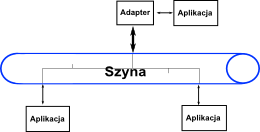
\includegraphics[bb=0 0 208 106]{chapter1/esb.png}
% % esb.png: 260x132 pixel, 90dpi, 7.34x3.73 cm, bb=0 0 208 106
% \caption{Zasada dzia�ania ESB \cite{esb:sojbi}}
% \label{fig:esb}
%\end{figure}

\begin{figure}[htb!]
 \centering
 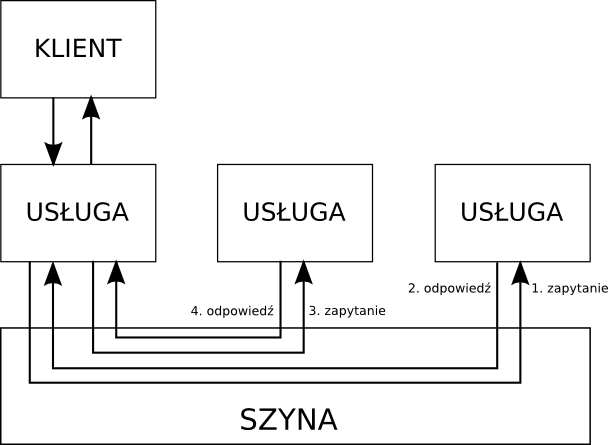
\includegraphics[bb=0 0 233 170]{chapter1/esb2.png}
 % esb2.png: 608x445 pixel, 188dpi, 8.21x6.01 cm, bb=0 0 233 170
 \caption{Zasada dzia�ania ESB \cite{esb:sojbi}}
 \label{fig:esb}
\end{figure}


\subsection{Historia ESB}
ESB powsta�o na bazie scharakteryzowanych poni�ej, bardzo obecnie popularnych koncepcji MOM i EAI. 
% Poni�ej znajduje si� ich kr�tka charakterystyka.

% Na kszta�t ESB mia�o wp�yw wiele do�wiadcze� z wcze�niejszych pr�b kompleksowego podej�cia 
% do problemu integracji us�ug. Najbardziej znacz�cy wk�ad mia�y koncepcje MOM oraz EAI:

\paragraph{Message Oriented Middleware}
to architektura kt�rej rozw�j rozpocz�� si� na pocz�tku lat 80 i trwa do dzi�. Opiera si� ona na koncepcji asynchronicznej wymiany jednostek danych (wiadomo�ci) za pomoc� jednolitych protoko��w komunikacyjnych. % zastanowi� si� czy jednolitych i czy wiadomo�ci czy komunikaty
Podstawowymi trybami komunikacji MOM s�: % bo mog� by� inne
\begin{itemize}
\item  Point-to-Point (punkt-punkt) - tryb w kt�rym istnieje tylko jeden
producent i jeden konsument wiadomo�ci
\item  Publish/Subscribe (publikuj/zapisz si�) - tryb w kt�rym istnieje jeden
producent, a odbiorc�w mo�e by� dowolna ilo��.
\end{itemize}

U�ycie rozwi�za� MOM sta�o si� standardem obs�ugi asynchronicznych zdarze� w du�ych aplikacjach biznesowych, stymuluj�c jednocze�nie ich rozw�j. Wiele z nich posiada tak zaawansowane w�a�ciwo�ci jak: niezawodno�� dostarczania, kolejkowanie i filtrowanie wiadomo�ci, transakcyjno��, mo�liwo�� klastrowania, czy zaawansowane mechanizmy bezpiecze�stwa. 

Do standard�w realizuj�cych ide� MOM nale�� mi�dzy innymi:JMS (Java Messaging System) \cite{esb:mom:jms}, IceStorm \cite{esb:mom:icestorm}, CORBA Notification Service \cite{esb:mom:corba}, Microsoft MSQM \cite{esb:mom:msqm} oraz specyfikacje WS-Events \cite{esb:mom:wsevents} i WS-Notifications \cite{esb:mom:wsnotifications}.

\begin{figure}[h!tb]
 \centering
 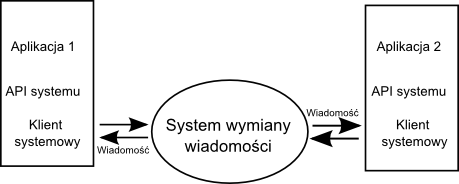
\includegraphics[bb=0 0 221 88]{chapter1/mom.png}
 % mom.png: 273x109 pixel, 89dpi, 7.79x3.11 cm, bb=0 0 221 88
 %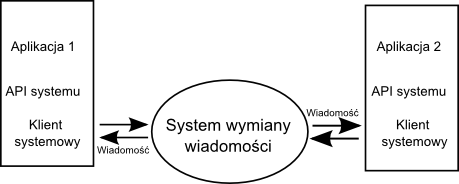
\includegraphics[bb=0 0 203 88]{chapter1/mom.png}
 %% mom.png: 251x109 pixel, 89dpi, 7.16x3.11 cm, bb=0 0 203 88
 \caption{Zasada dzia�ania MOM}
 \label{fig:mom}
\end{figure}


% Dzi�ki du�ej popularno�ci rozwi�za� typu MOM, wiele doczeka�o si� w�a�ciwo�ci
% kt�re powoduj�, �e s� one z powodzeniem wykorzystywane w aplikacjach o du�ych wymaganiach - takich jak:
% nie jest to po polsku
% du�a popularno�� rozw. MOM zaowocowa�a ich dalszym rozwojem i wzbogacaniem o nowe wlasciwosci!!!

% \begin{itemize}
% \item  \textbf{niezawodno�� dostarczania wiadomo�ci} zapewniana przez za�o�enie,
% ka�da wiadomo�� jest autonomiczna (tj. w momencie jej wys�ania rola aplikacji w
% przetwarzaniu danego elementu ko�czy si�) oraz przez zastosowanie:
% \begin{itemize}
% \item  kolejkowania i zapewnienia dostarczenia, tzw. mechanizm
% store-and-forward, kt�ry powoduje, �e wiadomo�� dociera do adresata nawet je�li
% do��czy on do kana�u informacyjnego dopiero po jakim� czasie od wys�ania
% wiadomo�ci \footnote{du�e znaczenie ma tutaj tzw. persystencja wiadomo�ci celem
% jej dalszego u�ycia}
% \item  mechanizm�w potwierdze� pozwalaj�cych wysy�aj�cemu upewni� si�, �e
% wiadomo�� dotar�a do adresata
% \end{itemize}
% 
% \item \textbf{filtrowanie wiadomo�ci} na podstawie p�l nag��wka
% 
% \item \textbf{hierarchiczno�� temat�w} mechanizmu publish/subscribe - polega na
% tym �e wiadomo�ci
% wysy�ane do temat�w nadrz�dnych trafiaj� do jego wszystkich podga��zi
% \item \textbf{mechanizmy autoryzacji} wysy�ania i odbierania wiadomo�ci w
% oparciu o ACL z uwzgl�dnieniem hierarchi temat�w
% \item \textbf{obs�uga transakcyjno�ci} tzn. dostarczanie wiadomo�ci jest
% % co z t� transakcyjno�ci� 
% zablokowane do czasu, a� transakcja zostanie zako�czone oraz wszystkie
% wiadomo�ci zostan� pomy�lnie wys�ane 
% \end{itemize}

% napisac o dodatkowych wlasciwosciach niefunkcjonalnych tak jak load-balancing, fail-over...

\paragraph{EAI}
Enterprise Application Integration, to idea kt�ra pojawi�a si� w po�owie lat 90. Celem jaki przy�wieca� jej tw�rcom by�a redukcja ilo�ci koniecznych po��cze�
w systemie rozproszonym poprzez wprowadzenie jednego centralnego punktu tzw. hub-and-spoke broker (pol. po�rednik w strukturze gwia�dzistej). Na punkcie tym spoczywa zadanie zawiadywania ca�� komunikacj� w obr�bie systemu - to on decyduje o tym gdzie ma trafi� dana wiadomo��. Architektura ta separuje aplikacj� od w�a�ciwego kodu integruj�cego poprzez u�ycie oprogramowania BPM (Business Process Management)\cite{esb:bpm}.
\begin{figure}[h!tb]
 \centering
 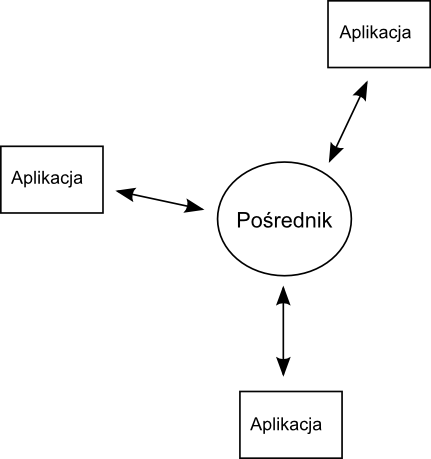
\includegraphics[bb=0 0 207 221]{chapter1/eai.png}
 % eai.png: 256x273 pixel, 89dpi, 7.31x7.79 cm, bb=0 0 207 221
 \caption{Zasada dzia�ania EAI \cite{esb:book:chapell}}
 \label{fig:eai}
\end{figure}

W za�o�eniach EAI mia�a by� stosowana w nast�puj�cych przypadkach:
\begin{itemize}
 \item Integracja proces�w biznesowych - zapewnienie ��czno�ci pomi�dzy
 procesami biznesowymi aplikacji istniej�cych w du�ych systemach
 \item Zapewnianie integralno�ci danych w r�nych cz�ciach systemu\footnote{Znane r�wnie� pod terminem EII (Enterprise Information
 	 Integration)}
 \item Uniezale�nienie implementacji od system�w zewn�trznych - przeniesienie 
 regu� i polityk biznesowych do EAI, tak aby zmiany dostawc�w nie wp�ywa�y na
  inne cz�ci
 systemu
 \item Udost�pnienie ujednoliconego interfejsu dla z�o�onych aplikacji
\end{itemize}

Istnieje wiele implementacji EAI, w�r�d najbardziej znanych znajduj� si�:
Microsoft BizTalk Server\texttrademark, SAP Exchange Infrastructure (SAP XI) \texttrademark oraz webMethods Integration Server \texttrademark.

% \subsection{ESB jako potomek MOM i EAI}
% ESB jako koncepcja maj�ca swe podwaliny w obu tych podej�ciach. Z MoM zaczerpn�a komunikacj� w oparciu o rozproszon� infrastruktur�, oddzielaj�c jednocze�nie mechanizm regu� systemowych (biznesowych) od implementacji poszczeg�lnych cz�ci systemu:

\paragraph{ESB jest pochodn� obu technologii}

\begin{figure}[h!tb]
 \centering
 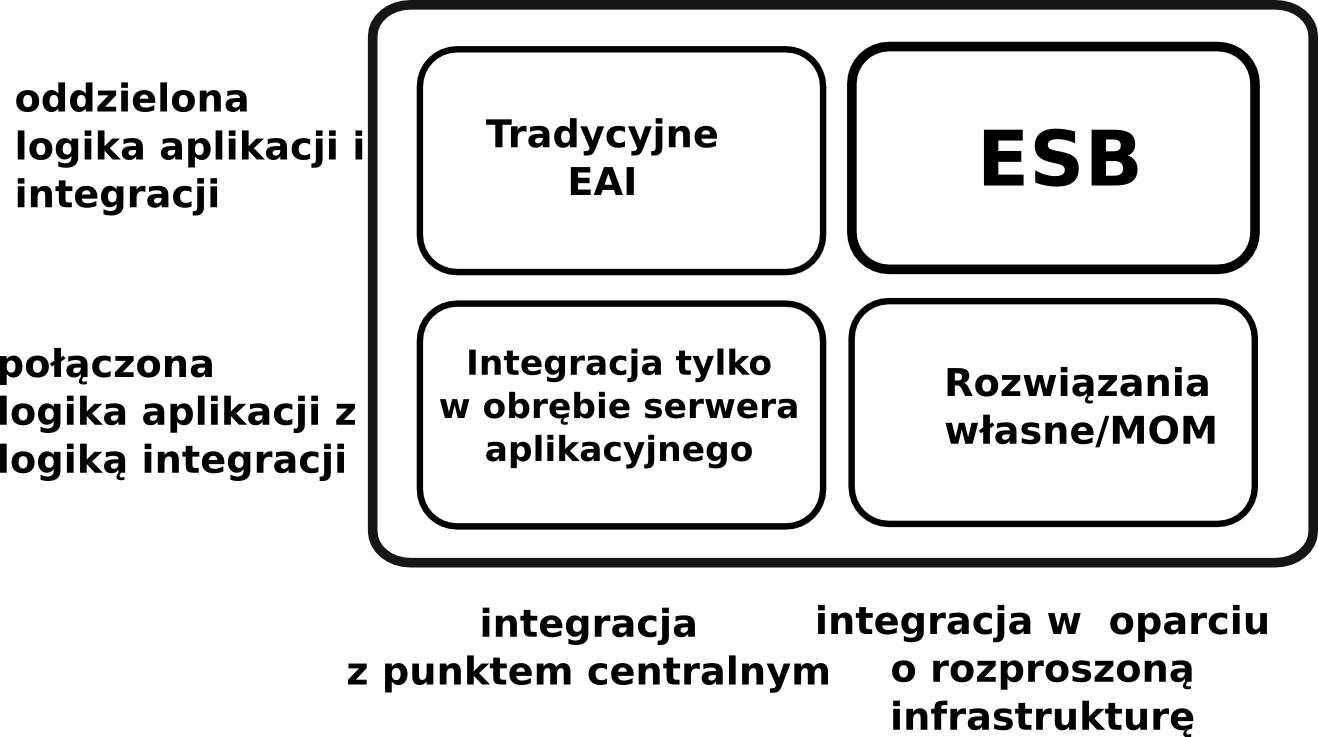
\includegraphics[bb=0 0 317 177]{chapter1/esb-where.png}
 % esb-where.png: 1318x737 pixel, 300dpi, 11.17x6.24 cm, bb=0 0 317 177
 \label{fig:esb_where}
 \caption{ESB jako pochodna EAI i MOM}
\end{figure}

Rysunek \ref{fig:esb_where} obrazuje spos�b w jaki ESB czerpa�o swoje cechy z obu podej��. Korzysta z charakterystycznej dla MOM rozproszonej infrastruktury dostarczania wiadomo�ci oraz oddziela logik� dostarczania od ich w�a�ciwego przetwarzania, co jest specyficzne dla EAI.

\subsection{Za�o�enia i cechy ESB}

Jednym z najwa�niejszych zamierze� tw�rc�w ESB by�o osi�gniecie mo�liwo�ci zastosowania tego rozwi�zania w najwi�kszej liczbie przypadk�w. Dlatego te� idea ESB opiera si� na nast�puj�cych za�o�eniach:
\begin{itemize}
	\item adaptowalno�� niezale�na od warunk�w wdro�enia - skali,
 technologii uczestnicz�cych czy sposobu modelowania aplikacji
	\item zunifikowane podej�cie do po��czenia poszczeg�lnych element�w 
oprogramowania
	\item �atwo�� integracji z oprogramowaniem zar�wno wewn�trz, jak i na 
zewn�trz korporacji
	\item prostota tworzenia aplikacji i dodawania do ju� istniej�cego
	 rozwi�zania
	\item zdecentralizowanie dzia�ania us�ug integracyjnych
	\item zwi�kszona przejrzysto�� systemu
	\item du�a elastyczno�� i �atwo�� reagowania na zmieniaj�ce si�
	wymagania
	\item zapewnienie du�ej skalowalno�ci tworzonych rozwi�za�.
\end{itemize}

% nie ma tu co napisac na koncu

\paragraph{Cechy ESB}
Z uwagi na fakt, i� koncepcja ESB nie jest poparta �adnym standardem, nie da si� wyr�ni� mo�liwo�ci jakich takie oprogramowanie winno dostarcza�. 
Istnieje jednak pewien ustalony zakres funkcjonalno�ci i cech, kt�re takie rozwi�zanie zwyk�o spe�nia�. Do takich nale�� \cite{esb:book:chapell}:
\begin{itemize}
 \item \textbf{Autonomiczno�� z mo�liwo�ci� dost�pu z zewn�trz}
 \item \textbf{Bezpiecze�stwo i niezawodno��}
 \item \textbf{Integracja oparta o uznane standardy} - do tych standard�w nale��
  \begin{itemize}
    \item XML - najpowszechniej u�ywany obecnie j�zyk opisu danych, wraz z j�zykami
     wspomagaj�cymi jego u�ycie, tj. XSD, XPath czy XSLT
    \item WSDL - zwyczajowo stosowany do opisu interfejs�w us�ug
    \item Standardy dost�pu do danych tj. LDAP, SQL czy RSS
    \item Standardy wymiany danych tj. SOAP, REST, DCOM czy XMPP
    \item Standardy transformacji danych tj. XSLT czy stosowany w hurtowniach
     danych (ang. data warehouses) ETL
  \end{itemize}
 \item{\textbf{Dostarczenie ustalonego zestawu funkcjonalno�ci}, w kt�ry zwyczajowo wchodz�:}
 \begin{itemize}
  \item \textbf{Mo�liwo�� sterowania procesem wykonania} - z u�yciem takich standard�w jak
   WS-BPEL, WS-Choreography czy (mniej popularnego) ebXML BPSS.
  \item \textbf{Rozproszone transformacje danych}
  \item \textbf{Przetwarzanie danych w czasie rzeczywistym} - mo�liwo�� definiowania reakcji 
  na konkretne warto�ci lub trendy danych
  \item \textbf{Zdalna konfiguracja}
  \item \textbf{Zdalne zarz�dzanie}
  \item \textbf{Monitorowanie}.
 \end{itemize}
\end{itemize}

% zdanie wienczace

% http://www.sonicsoftware.com/solutions/service_oriented_architecture/enterprise_service_bus/index.ssp

% \subparagraph{Du�y zasi�g rozwi�zania}
% Rozwi�zanie tworzy jedn� powszechn� sie� integracyjn� dla ca�ego systemu. Aplikacje w prosty spos�b 
% mog� do��czy� do szyny, i wymienia� dane z pozosta�ymi. Co wa�ne, nie jest konieczne aby ju� istniej�ce
% aplikacje by�y adaptowane specjalnie dla ESB - szyna w zamierzeniach powinna obs�ugiwa� jak najwi�cej 
% metod komunikacji.

% \subparagraph{Rozproszone transformacje danych}
% Kluczow� cz�ci� integracji aplikacji jest konwersja miedzy u�ywanmi przez nie formatami. Modu�y 
% za to odpowiadaj�ce rozwi�zuj� wiele problem�w zwi�zanych z enkapsulacj�, niepasuj�cymi typami danych, czy r�nicami w ich strukturach\footnote{Wi�cej informacji na ten temat mo�na znale�� na stronie: http://en.wikipedia.org/wiki/Object-Relational\_impedance\_mismatch}.

% \subparagraph{Realizacja SOA sterowanego zdarzeniami}
% Realizuj�c SOA w oparciu o ESB aplikacje, i us�ugi integracyjne s� traktowane jako abstrakcyjne 
% ``ko�c�wki'', kt�rych jedynym zadaniem jest przyj�cie danych w jakim� formacie, i odes�anie odpowiedzi
% po ich przetworzeniu. Maj�c tak sformu�owane podej�cie mo�emy powiedzie�, �e ESB w pe�ni wspiera 
% tworzenie aplikacji o architekturze SOA, z takimi zaletami jak lu�ne wi�zanie czy ponowne u�ycie.

% \subparagraph{Orchiestracja}
% ESB pozwala na orchiestracj� proces�w, tj. na sterowanie kolejno�cia wywo�a� i wymian� danych pomi�dzy
% poszczeg�lnymi aplikacjami i serwisami integracyjnymi (tzw. process flow). Maj�c tak� mo�liwo�� 
% �atwe staje si� zarz�dzanie zmianami w definicjach przep�yw�w w obr�bie systemu, a dzia�anie systemu
% zyskuje na przejrzysto�ci.

% \subparagraph{Bezpiecze�stwo i niezawodno��}
% Po��czenia w obr�bie szyny, jak r�wnie� poza ni� mog� by� bardzo silnie szyfrowane. Dodatkowo maj�c jednolite rozwi�zanie integracyjne, �atwiejsze staje si� opracowywanie polityk bezpiecze�stwa. 
% Niezawodno�� ESB jest oparta o fakt, i� trzon tego rozwi�zania pozostaj� ju� bardzo dojrza�e i pewne rozwi�zania MOM.

% \subparagraph{Autonomiczno�� z mo�liwo�ci� po��czenia na zewn�trz}
% W przeciwie�stwie do EAI, kt�re wymaga�o od wszystkich podsystem�w po��czenia do jednego punktu centralnego, ESB pozwala na naturalniejszy podzia� aplikacji w obr�bie systemu - mo�liwe jest takie 
% zorganizowanie integracji, by ka�da jednostka organizacyjna posiada�a w�asn� szyn�, odr�bn� szyn�, a interakcje odbywa�y si� z udzia�em sieci integracynej wy�szego szczebla (r�wnie� szyny ESB). Dzia�anie 
% takie pozwala na lu�niejsze powi�zanie pomi�dzy podsystemami, i co za tym idzie pe�niejsze wype�nienie
% paradygmatu SOA. 

% \subparagraph{Zdalna konfiguracja, zarz�dzanie i monitorowanie}
% Poniewa� ESB w za�o�eniach jest technologi� integracyjn� wdra�an� u r�nych klient�w, jej przydatn�
%  w�a�ciwo�ci� jest mo�liwo�� jej zdalna obs�ugi. Wa�ne jest aby szyna udost�pnia�a 
% pe�ne mo�liwo��i
%  konfiguracji ju� istniej�cych i dodawania nowych element�w do szyny. Inn� wa�na
%  w�a�ciwo�ci�, jest 
% mo�liwo�� wgl�du w parametry pracy systemu, takie jak przepustowo��, obci��enie poszczeg�lnych komponent�w, czy stopa b��d�w.

% \subparagraph{Obs�uga pewnej klasy szerzej przyj�tych standard�w}
% ESB powsta�o z zamiarem wykorzystania ju� istniej�cych standard�w. Obejmuj� one r�ne klasy zagadnie�
% integracji:

% \subparagraph{U�ycie j�zyka XML}
% XML jest podstawowym formatem danych u�ywanym w ESB. Jego wieloplatformowe wsparcie i powszechne uznanie,
%  czyni go w zasadzie jedynym wyborem. Dodatkowym czynnikiem wp�ywaj�cym na u�ycie XML jest mnogo��
%  technologii, kt�re powsta�y wok� tego j�zyka, takie jak szeroko stosowany SOAP, czy bardzo dobrze
%  rozwini�te mechanizmy transformacji takie jak XSLT.
% 
% \subparagraph{Protoko�y transportu i dost�pu do danych}
% Chc�c zapewni� jak najwy�sz� integracj� z r�nymi systemami ESB musi obs�ugiwa� szerok� gam� tego typu
% standard�w. W obecnym czasie nale�� do nich przede wszystkim protoko�y coraz popularniejszych w
%  ostatnim czasie WebService'�w, takie SOAP czy REST. Wa�nym, i cz�sto obs�ugiwanym standardem jest
%  r�wniez wspomniany wcze�niej JMS. Do gamy proko��w nale�� r�wnie� takie protoko�y jak:
% \begin{itemize}
%  \item file - monitorowanie plik�w w systemie plik�w na jakim� serwerze
%  \item bazodanowe JDBC czy LDAP - mo�liwo�� reagowania na pojawiaj�ce si� dane poprzez wykonywanie co
%  jaki� czas danego zapytania SQL
%  \item DCOM
%  \item RSS
%  \item SIP
%  \item XMPP
%  \item TCPIP
% \end{itemize}
% i wiele innych standard�w. Taka mnogo�� standard�w pozwala daje du�e mo�liwo�ci je�li chodzi o interakcje
% z istniej�cymi podsystemami.

% \subparagraph{Standardy tranformacji danymi}
% Standardowo obs�ugiwane s� jezyki XPath i XQuery, oraz przeznaczony do transformacji plik�w XML j�zyk XSLT. 
% Innym cz�sto obs�ugiwanym standardem jest przyj�ty w hurtowniach danych standard ETL (Extract, Transform, Load).

% \subparagraph{Standardy sterowania procesem wykonania}
% Czyli standardy opisuj�ce sposoby sterowania orchiestracj� us�ug. Najsze�ciej obs�ugiwanym jest opisywany dalej BPEL. Czasem jest to r�wnie� WS-Choreography czy (mniej popularny) ebXML BPSS.
% http://www-306.ibm.com/software/info1/websphere/index.jsp?tab\=landings\/esb

% \subparagraph{WSDL}
% Wa�nym standardem pojawiaj�cym si� w ka�dej implementacji ESB jest j�zyk WSDL, pozwalaj�cy na 
% opis interfejs�w us�ug, udost�pnianych przez aplikacje.

% \subparagraph{Przetwarzanie danych w czasie rzeczywistym}
% Jest to cecha kt�ra w ostatnim czasie staje si� coraz popularniejszym elementem ESB. Funkcjonalno�� ta
% opiera si� na definiowaniu dzia�a� b�d�cych reakcj� na dane przep�ywaj�ce przez szyne. Mo�e by� to na przyk�ad powiadomienie o niskim stanie magazynowym, czy tendencji spadkowej jakiego� waloru na gie�dzie.s

\subsection{Istniej�ce implementacje ESB}
Na rynku istnieje wiele implementacji ESB. Do najbardziej znanych nale��:

\begin{itemize}
  \item Sonic ESB - najstarsza implementacja ESB 
\cite{esb:impl:sonic}
 \item OpenESB (Glassfish) \cite{esb:impl:openesb}
 \item JBoss ESB \cite{esb:impl:jbossesb}
 \item WebSphere ESB \cite{esb:impl:websphere}
 \item MULE \cite{esb:impl:mule}
 \item Apache ServiceMix \cite{esb:impl:servicemix}
 \item BEA Aqualogic Service Bus \cite{esb:impl:aqualogic}
\end{itemize}

Autorzy przeanalizowali powy�sze rozwi�zania pod k�tem wymaga� pracy, zwracaj�c najwi�ksz� uwag� na otwarto�� kodu i prostot� tworzenia aplikacji. Do realizacji pracy wybrano �rodowisko OpenESB.

\subsection{Wdro�enia ESB}
Mimo swojej kr�tkiej historii, wiele firm zaadaptowa�o ju� lub te� jest w trakcie adaptowania rozwi�za�
integracyjnych w oparciu o ESB. Do godnych uwagi nale��:
\begin{itemize}
 \item Wdro�enie ESB w infrastrukturze jednego z wiod�cych po�yczkodawc�w w Stanach Zjednoczonych,
 	pozwoli�o na obni�enie koszt�w przetwarzania danych o 60\%. Dokonano tego 
poprzez oparcie o ESB
	jednolitego systemu informacji o klientach spinaj�cego rozsiane po ca�ym
 kraju biura kredytowe
 	oraz system eCredit. \cite{esb:book:chapell}
 \item Trwaj�ce 3 tygodnie wdro�enie ESB w jednej z najwi�kszych sieci dystrybucji �ywno�ci w Europie,
 pozwoli�o na zaoszcz�dzenie 3 milion�w dolar�w. Rol� ESB by�o zintegrowanie system�w trzech r�nych 
system�w informatycznych, celem automatyzacji zakupu, sprzeda�y i zarz�dzania logistyk�.
 \item Jedna z najwi�kszych firm energetycznych w Stanach Zjednoczonych (10 miliard�w dolar�w obrotu
 rocznie), u�ywa ESB w rachunkowo�ci, zarz�dzaniu systemem i raportowaniu. Dodatkowo na ESB oparta jest 
 realizacja regulowanej prawnie komunikacji z rz�dem. \cite{esb:book:chapell}
 \item Udzia� ESB w integracji system�w kom�rek rz�dowych Stan�w Zjednoczonych celem walki z terroryzmem
w ramach dokumentu ``USA Patriot Act''. \cite{esb:book:chapell}
% http://www.gcn.com/print/25_20/41319-1.html - Washington DC
\end{itemize}

Istnienie wdro�e� o znaczeniu krytycznym �wiadczy, o du�ych mo�liwo�ciach koncepcji ESB, w kontek�cie rozwi�za� tego typu.

% http://steve.vinoski.net/blog/2007/10/04/the\-esb\-question/
% http://www.oreillynet.com/xml/blog/2006/08/esb\_adoption\_in\_government.html
\subsubsection{Problemy ESB}
Zaawansowanie koncepcji ESB poci�ga za sob� szereg problem�w w�r�d kt�rych najbardziej znacz�ce to:
\begin{itemize}
 \item Spowodowany kr�tk� histori� technologii, brak odpowiedniej ilo�ci ekspert�w dysponuj�cych wiedz�
wystarczaj�c� do zarz�dzania i konfiguracji ESB
 \item Wa�ny w kontek�cie tej pracy, du�y narzut technologiczny - bior�c pod uwag� u�ycie takich koncepcji jak orchiestracja, czy transformacje XSLT, przy dodatkowym wykorzystaniu us�ug webservice zbudowanych w oparciu technologi� SOAP, istnieje du�a obawa, �e obci��enie generowane przez samo oprogramowanie warstwy po�rednicz�cej, mo�e by� znacz�ce.
\end{itemize}


% 
% \begin{itemize}
% 	\item  problemy ESB (conieco o wydajno�ci)
% 	% \item  istniej�ce implementacje ESB %
% % http://www-306.ibm.com/software/info1/websphere/index.jsp\?tab\=landings\/esb
% 	\item  zastosowania ESB w prawdziwym �wiecie:
% \end{itemize}




% http://www.gcn.com/print/25_20/41319-1.html


\subsection{JBI}

JBI (Java Business Integration) - to specyfikacja JCP\footnote{JSR-208 (Java Specification Request) tworzony przez takie firmy jak Syn Microsystems, BEA, Borland, Nokia, Novell czy Oracle\cite{esb:jbi:jsr}}(Java Community Process), kt�ra pozwala na stworzenie �rodowiska realizuj�cego za�o�enia ESB w technologiach zwi�zanych z j�zykiem Java. Definiuje on �rodowisko komponent�w realizuj�cych model wymiany danych oparty o specyfikacj� WSDL 2.0\cite{ws:wsdl:spec}.
Specyfikacja stanowi, i� komponenty JBI musz� posiada� nast�puj�ce trzy cechy:
\begin{itemize}
 \item \textbf{Przeno�no��} pomi�dzy r�nymi implementacjami kontenera JBI
 \item \textbf{Scentralizowane zarz�dzanie}
 \item \textbf{Wsp�praca z innymi komponentami} w obr�bie kontenera, niezale�nie od tego 
 sk�d pochodz�
\end{itemize}
Ka�dy z komponent�w realizuje funkcj� dostawcy i/lub konsumenta us�ugi\cite{esb:jbi:jbi_components_theory}\cite{esb:jbi:developing_jbi}.

% https://open-esb.dev.java.net/kb/preview4/jbiag.html
% http://www.scribd.com/doc/257973/JBI-based-ESB-as-backbone-for-SOI-applications
% ksi��ka o JBI

% Proponuj� spojrze� do ksi��ki rozdzia� 10.1 oraz do dokumentacji glassfisha

Podstawow� nomenklatur� JBI przedstawia rysunek \ref{fig:jbi-simple}; wyr�nia ona nast�puj�ce elementy:

\begin{figure}[h!]
 \centering
 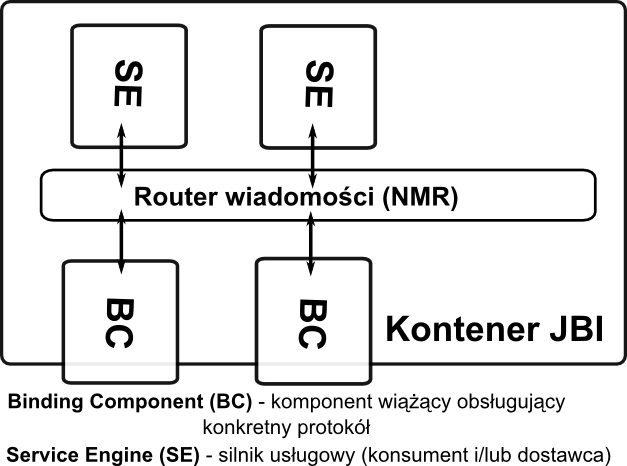
\includegraphics[bb=0 0 300 223]{chapter1/jbi-simple.png}
 % jbi-simple.png: 675x502 pixel, 94dpi, 18.26x13.58 cm, bb=0 0 518 385
 \caption{Nomenklatura JBI\cite{esb:jbi:jbi_components_theory}}
 \label{fig:jbi-simple}
\end{figure}

\paragraph{Jednostka us�ugowa (SU)} (org. service unit) - to jednostka programowa dostarczaj�ca konkretnej implementacji us�ug korzystaj�ca z w�a�ciwo�ci kontenera w kt�rym zosta�a umieszczona. Aplikacje sk�adaj� si� ze skomponowanych SU umieszczonych w kontenerach �rodowiska JBI.

\paragraph{Silniki us�ugowe (SE)} (org. service engine) - to komponenty wykonawcze umieszczane w kontenerze JBI, kt�rych zadaniem jest dostarczanie lub korzystanie z us�ug w jego obr�bie.
Komponenty te dostarczaj� w�a�ciwej logiki takiej jak obs�uga transformacji, regu� biznesowych czy j�zyk�w skryptowych. SE pe�ni� rol� kontener�w dla SU.

\paragraph{Komponenty wi���ce (BC)} (org. binding component) - to komponenty zapewniaj�ce ��czno�� kontenera ze �wiatem zewn�trznym w obu kierunkach - ka�dy z nich realizuje okre�lony protok� komunikacyjny. Wiadomo�ci s� transformowane i przekazywane z i do NMR, kt�ry decyduje o jej dalszej drodze. Takie podej�cie, pozwala ka�demy SE komunikowa� si� ze �wiatem zewn�trznym z pomoc� dowolnego obs�ugiwanego przez kontener protoko�u. Podobnie jak SE, BC r�wnie� pe�ni� rol� kontener�w dla SU.

\paragraph{Router wiadomo�ci o jednolitym formacie (NMR)}(org. Normalized Message Router) -
najwa�niejsza cz�� �rodowiska JBI - stanowi element kt�ry zajmuje si� sterowaniem przep�ywem wiadomo�ci z punkt�w �r�d�owych do punkt�w docelowych, na podstawie okre�lonego z g�ry kontraktu. NMR mo�e r�wnie� realizowa� pewne funkcje QoS dotycz�ce dostarczania wiadomo�ci w obr�bie kontenera.

\paragraph{Kontener JBI} (org. JBI Container) - �rodowisko wykonawcze komponent�w JBI - zar�wno BC jak i SE. 

\subsubsection{Kontrakt}
Implementuj�c komponent JBI, realizujemy pewien kontrakt, kt�ry obejmuje zagadnienia instalacji, pakowania, zarz�dzania cyklem �ycia, publikacji oferowanych us�ugi i przetwarzania wiadomo�ci bazuj�ce na jednym z czterech MEP (Message Exchange Pattern)\footnote{opcjonalnie do kontraktu mo�e nale�e� r�wnie� zarz�dzanie jednostk� us�ugow� (SU - z ang. service unit)}.

\paragraph{MEP - wzorce wymiany wiadomo�ci}
NMR dostarcza wiadomo�ci realizuj�c jeden z czterech wzorc�w wymiany wiadomo�ci b�d�cych cz�ci� specyfikacji WSDL 2.0\cite{ws:wsdl:spec}\cite{esb:sojbi}:

\begin{itemize}
 \item \textbf{In-Only} - standardowy spos�b przesy�ania w jedn� stron�, w kt�rym konsument wysy�a 
 wiadomo�� do dostawcy us�ugi, kt�ry odpowiada statusem 
 \item \textbf{Robust In-Only} - niezawodny spos�b przesy�ania jednokierunkowego, w kt�rym konsument
wysy�a wiadomo�� do dostawcy, kt�ry odpowiada statusem, i je�li jest to b��d (fault), odes�ane zostaje potwierdzenie
 \item \textbf{In-Out} - dwukierunkowy spos�b wymiany wiadomo�ci w kt�rym na wiadomo�� konsumenta,
dostawca us�ugi wysy�a odpowied� kt�ra jest nast�pnie potwierdzana
 \item \textbf{In Optional-Out} - dwukierunkowy spos�b wymiany wiadomo�ci, w kt�rym wiadomo�� b�d�ca 
 odpowiedzi� na ��danie konsumenta jest opcjonalna
\end{itemize}

\subsubsection{Implementacje JBI}
Najszerzej znane implementacje kontenera JBI to:
\begin{itemize}
 \item ServiceMix (FUSE ESB) \cite{esb:impl:servicemix}
 \item OpenJBI (OpenESB) \cite{esb:impl:openesb}
 \item JBossESB \cite{esb:impl:jbossesb}
 \item ObjectWeb2 PEtALS \cite{esb:impl:petals}
\end{itemize}
zgodny z JBI jest r�wnie� MULE \cite{esb:impl:mule}.

Do cel�w pracy wybrano implementacj� OpenJBI firmy Sun Microsystems\texttrademark.

\section{BPEL}
Aby w pe�ni korzysta� z zalet SOA, konieczne jest osi�gniecie niezale�no�ci kompozycji us�ug, od ich implementacji.\cite{bpel:book:bpel4ws}

Istniej� dwa podej�cia do tego zagadnienia \cite{bpel:book:wsbpel}:
\begin{itemize}
 \item \textbf{Orchiestracja} - w kt�rej jeden centralny komponent przejmuje kontrol� nad us�ugami 
 b�d�cymi uczestnikami procesu biznesowego, koordynuj�c ich wsp�prac�. Us�ugi nie s� �wiadome bycia
  uczestnikami procesu biznesowego (przyk�ad ilustruje rys \ref{fig:bpel_orchiestracja}).
  \begin{figure}[h!tb]
   \centering
   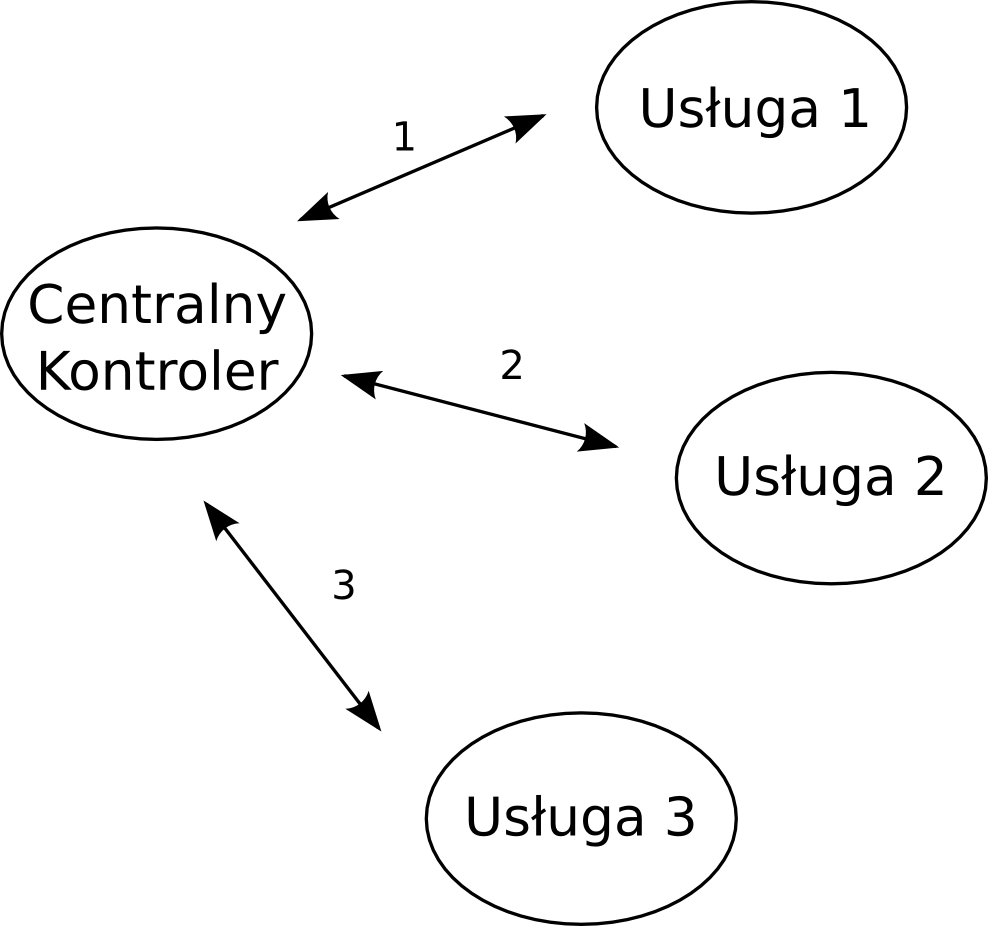
\includegraphics[bb=0 0 237 222]{chapter1/orchiestracja.png}
   % orchiestracja.png: 306x287 pixel, 93dpi, 8.36x7.84 cm, bb=0 0 237 222
   %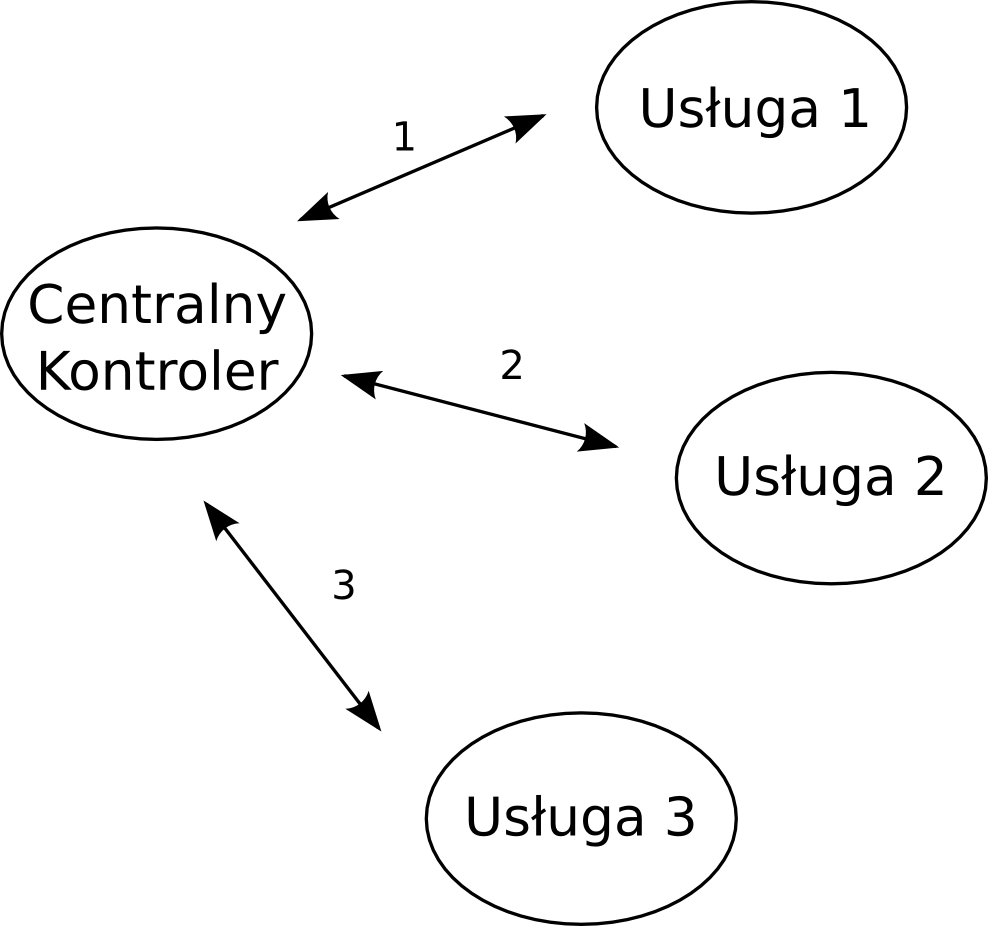
\includegraphics[bb=0 0 311 238]{chapter1/orchiestracja.png}
   %% orchiestracja.png: 384x294 pixel, 89dpi, 10.96x8.39 cm, bb=0 0 311 238
   \caption{Orchiestracja}
   \label{fig:bpel_orchiestracja}
  \end{figure}

 \item \textbf{Choreografia} - podej�cie w kt�rym zamiast jednego centralnego punktu, ka�da us�uga wie
kiedy i z jakimi us�ugami ma si� komunikowa�. Us�ugi musz� by� �wiadome uczestniczenia w procesie biznesowym (przyk�ad ilustruje rysunek \ref{fig:bpel_choreografia}).
\begin{figure}[htb!]
 \centering
 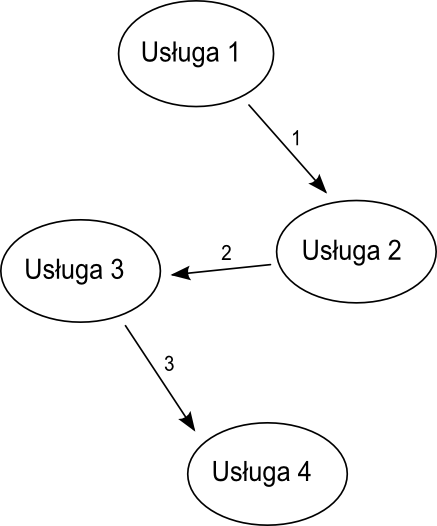
\includegraphics[bb=0 0 210 252]{chapter1/choreografia.png}
 % choreografia.png: 271x326 pixel, 93dpi, 7.40x8.90 cm, bb=0 0 210 252
 %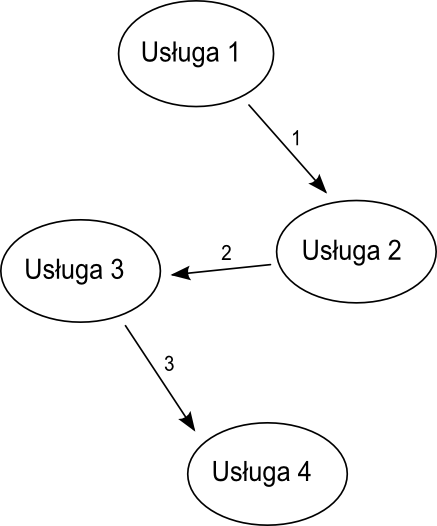
\includegraphics[bb=0 0 211 254]{chapter1/choreografia.png}
 % choreografia.png: 609x422 pixel, 93dpi, 16.63x11.53 cm, bb=0 0 472 327
 \caption{Choreografia}
 \label{fig:bpel_choreografia}
\end{figure}

\end{itemize}



% mo�e jaki� krotki tekst o tym ze �eby w pe�ni korzystac z SOA musimy jako� osi�gn�� kompozycje us�ug, i tu ew wymieni� podej�cie orchiestracji i choreografii, nastepnie napisa� o BPEL.
% Powstanie j�zyka BPEL mia�o zwi�zek z potrzeb� oddzielenia logiki element�w procesu od jego przebiegu.

% kr�tko wspomnie� o tym kto mia� wp�yw na powstanie j�zyka, 

\textbf{BPEL}\cite{bpel:spec} (Business Process Execution Language) jest to zdefiniowany przez organizacj� OASIS j�zyk orchiestracji proces�w biznesowych opartych o us�ugi zdefiniowane w j�zyku WSDL.

J�zyk ten pozwala na modelowanie na dw�ch poziomach abstrakcji: opisowym poziomie abstrakcyjnym(z ang. Abstract Business Process)\footnote{modele takie nie maj� by� wykonywane, a s� jedynie tworzone celem zobrazowania pewnego konkretnego procesu} i dok�adniejszym poziomie wykonania(z ang. Executable Business Process)\cite{bpel:spec}.

Interakcja z us�ugami w j�zyku BPEL odbywa si� na dwa sposoby:
\begin{itemize}
 \item eksport funkcjonalno�ci, wykonanie procesu BPEL jest zwykle wyzwalane poprzez ��danie wykonania operacji webservice
 \item import funkcjonalno�ci, proces BPEL umo�liwia wykonanie operacji na us�ugach webservice
\end{itemize}

\subsection{Wersje BPEL}

\paragraph{Wersje 1.0 i 1.1}
BPEL,a w zasadzie BPEL4WS (Business Process Execution Language for Web Services) powsta� w 2002 jako efekt wsp�pracy firm BEA, IBM i Microsoft. W roku 2003 do organizacji specyfikuj�cej BPEL do��czy�y firmy SAP oraz Siebel Systems, a j�zyk ewoluowa� do wersji 1.1. Wersja ta zosta�a zaaprobowana przez organizacj� OASIS (Organization for the Advancement of Structured Information Standards), i od tamtego czasu j�zyk ten sta� si� standardem w dziedzinie kompozycji proces�w biznesowych\cite{bpel:bpeljava}\cite{bpel:book:wsbpel}\cite{bpel:wikipedia}\cite{bpel:spec1.1}.

\subparagraph{Mo�liwo�ci j�zyka BPEL w wersji 1.1}
Specyfikacja j�zyka BPEL przewiduje nast�puj�ce mo�liwo�ci:

\begin{itemize}
 \item definiowanie typowanych zmiennych i synchronizowany dost�p do nich
 \item wykonywanie operacji webservice
 \item r�wnoleg�e wykonywanie operacji 
 \item definiowanie zasi�g�w (scope) dla zmiennych
 \item rzucanie i obs�ugiwanie wyj�tk�w
 \item dost�p do zmiennych za pomoc� wyra�e� XPath
 \item manipulacja zmiennymi
\end{itemize}

% ci�ko powiedziec co tu wstawi�

\subparagraph{Dost�pne konstrukcje} BPEL w wersji 1.1 oferuje nast�puj�ce konstrukcje:
\begin{itemize}
 \item \textbf{Proste}
 \begin{itemize}
  \item \textbf{Assign} przypisanie warto�ci zmiennej
  \item \textbf{Wait} oczekiwanie okre�lony okres czasu
  \item \textbf{Empty} instrukcja pusta
  \item \textbf{Throw} rzucenie wyj�tku
  \item \textbf{ReThrow} ponowne rzucenie z�apanego wyj�tku
  \item \textbf{Exit} zako�czenie procesu				 
  \item \textbf{Compensate} pozwalaj�ce na zdefiniowanie zachowania procesu w obr�bie transakcji, w przypadku, gdy jedna z jego sk�adowych zawiedzie (pr�ba odwr�cenia efekt�w dzia�ania element�w ju� wykonanych\footnote{analogiczne do zachowania transakcyjno�ci w bazach danych, tzw. ACID (skr�t ten pochodzi z terminologii baz danych, i oznacza cztery warunki jakie musz� spe�nia� transakcje: atomowo��, sp�jno��, izolacja i trwa�o�� (z ang. Atomicity, Consistency, Isolation, Durability)\cite{bpel:acid})})
 \end{itemize}
 \item \textbf{Strukturalne}
 \begin{itemize}
    \item \textbf{Sequence} wydzielony blok strukturalny
    \item \textbf{Scope} zasi�g zmiennej
    \item \textbf{If} instrukcja warunkowa
    \item \textbf{While} p�tla z warunkiem ewaluowanym na jej pocz�tku
    \item \textbf{Pick} oczekiwanie na jedno z zadeklarowanych zdarze�
    \item \textbf{Flow} wykonanie r�wnoleg�e
  \end{itemize}
  \item \textbf{Operacje na us�ugach webservice}
  \begin{itemize}
    \item \textbf{Receive} odebranie wiadomo�ci z us�ugi dostarczanej przez
     proces\footnote{operacja ta jest najcz�ciej operacj� wyzwalaj�c� proces}
    \item \textbf{Reply} odpowied� na odebran� wiadomo��\footnote{analogicznie
     operacja taka najcz�ciej ko�czy wyzwolony proces}
    \item \textbf{Invoke} wykonanie operacji na us�udze webservice.
  \end{itemize}
\end{itemize}


\subsubsection{Wersja 2.0}
Opracowana w roku 2004 nowa wersja j�zyka BPEL wprowadzi�a takie usprawnienia jak mo�liwo�� rozszerzania j�zyka, czy uproszczenia w przypisywaniu i inicjalizacji zmiennych. Pojawi�y si� nowe p�tle: RepeatUntil\footnote{p�tla z warunkiem ewaluowanym na jej ko�cu} i wykonywana zar�wno r�wnolegle, jak i sekwencyjnie ForEach\footnote{p�tla dokonuj�ca pewnych operacji na zbiorze danych}. Uproszczono r�wnie� obs�ug� b��d�w oraz inicjalizacj� tzw. Partner Link\footnote{odniesie� do us�ug w obr�bie proces�w}. Zmieniono r�wnie� oficjaln� nazw� j�zyka - obecnie oficjaln� nazw� jest WS-BPEL (Web Service - Business Process Execution Language)\footnote{uczyniono tak celem dopasowania si� do pozosta�ych nazw standard�w z zakresu technologii webservice kt�rych nazwy zwyczajowo zaczynaj� si� od ``WS-''}\cite{bpel:bpeljava}\cite{bpel:book:wsbpel}\cite{bpel:wikipedia}\cite{bpel:spec2}. \\
\\
Wszystkie dost�pne obecnie konstrukcje j�zyka BPEL, wraz z ich graficznymi reprezentacjami przedstawia rysunek \ref{fig:bpel_pallette}(nale�y mie� jednak na uwadze fakt, i� reprezentacje te nie stanowi� cz�ci standardu).

% \begin{figure}[h!tb]
%  \centering
%  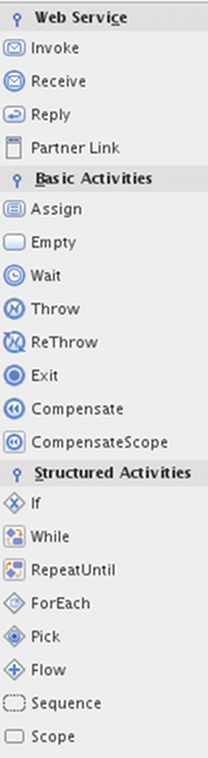
\includegraphics[width=200pt,bb=0 0 373 230]{chapter1/netbeans_pallette.png}
%  % netbeans_pallette.png: 373x230 pixel, 72dpi, 13.16x8.11 cm, bb=0 0 373 230
%  \caption{Elementy konstrukcyjne j�zyka BPEL}
%   \label{fig:bpel_pallette} 
% \end{figure}

\begin{figure}[h!kp]
 \centering
 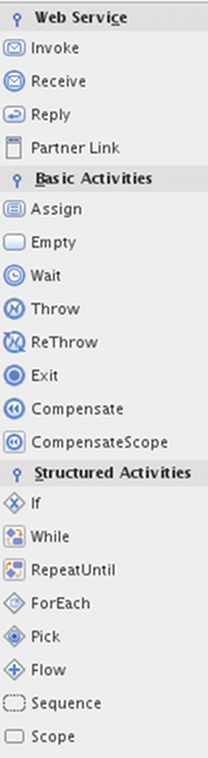
\includegraphics[bb=0 0 100 363]{chapter1/netbeans_pallette.png}
 % netbeans_pallette.png: 162x548 pixel, 72dpi, 5.71x19.33 cm, bb=0 0 162 548
 \caption{Elementy konstrukcyjne j�zyka BPEL}
 \label{fig:bpel_pallette}
\end{figure}



% \begin{figure}[htb]
%  \centering
%  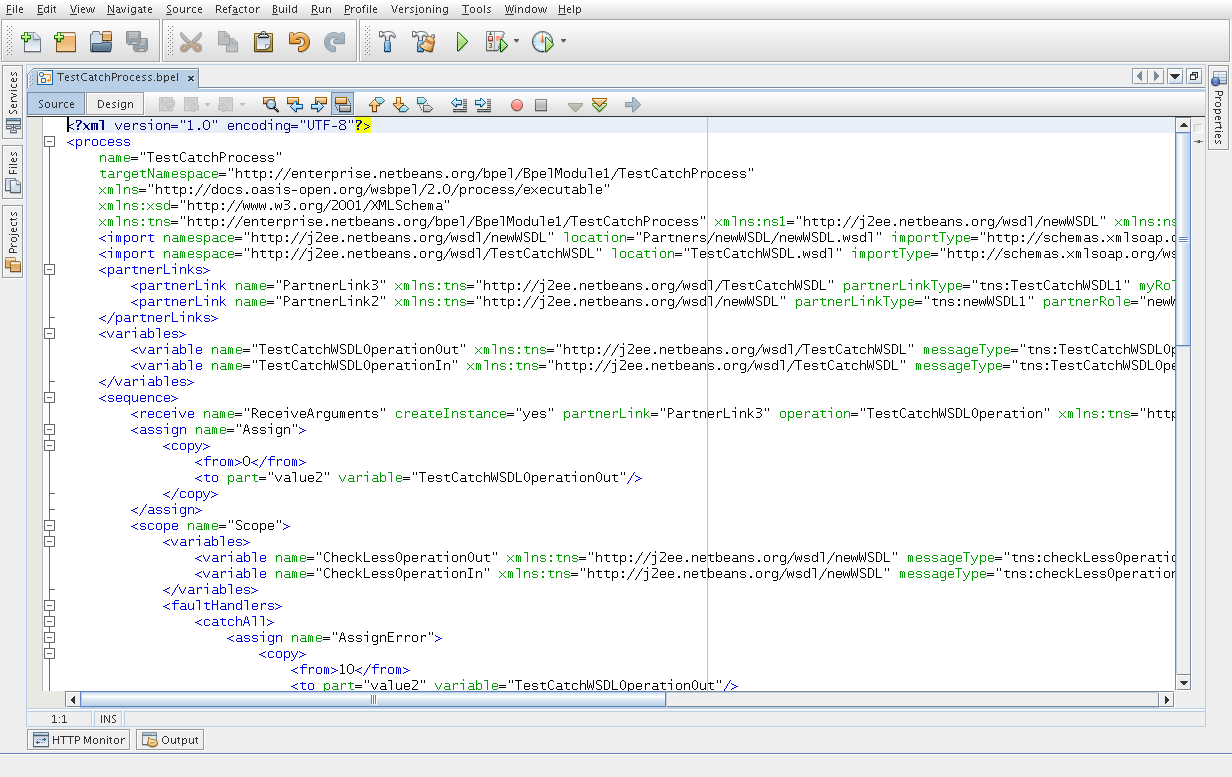
\includegraphics[width=12cm,height=8cm,bb=0 0 1232 777]{chapter1/bpel_src.png}
%  % bpel_src.png: 1232x777 pixel, 72dpi, 43.47x27.42 cm, bb=0 0 1232 777
%  \caption{Pakiet NetBeans - proces BPEL opisany w XML}
%  \label{fig:bpel_sample_src}
% \end{figure}

\subsection{Dost�pne implementacje BPEL}
J�zyk BPEL jest obs�ugiwany w wielu �rodowiskach integracyjnych, zar�wno jako komponenty, jak i samodzielne rozwi�zania. Do najbardziej rozwini�tych komercyjnych rozwi�za� nale��\cite{bpel:book:bpel4ws}:
\begin{itemize}
 \item IBM Websphere Business Integration Foundation\texttrademark\cite{esb:impl:websphere}
 \item Oracle BPEL Process Manager\texttrademark\cite{bpel:impl:oracle}
 \item Microsoft BizTalk\texttrademark\cite{bpel:impl:biztalk}
 \item BEA Aqualogic\texttrademark\cite{esb:impl:aqualogic}
\end{itemize}

Istnieje r�wnie� kilka rozwi�za� niekomercyjnych takich jak:
\begin{itemize}
 \item OpenESB BPEL JBI Component\cite{esb:impl:openesb}
 \item ActiveBPEL Engine\cite{bpel:impl:activebpel}
 \item Apache ODE\cite{bpel:impl:ode}
\end{itemize}

\begin{figure}[h!kp]
 \centering
 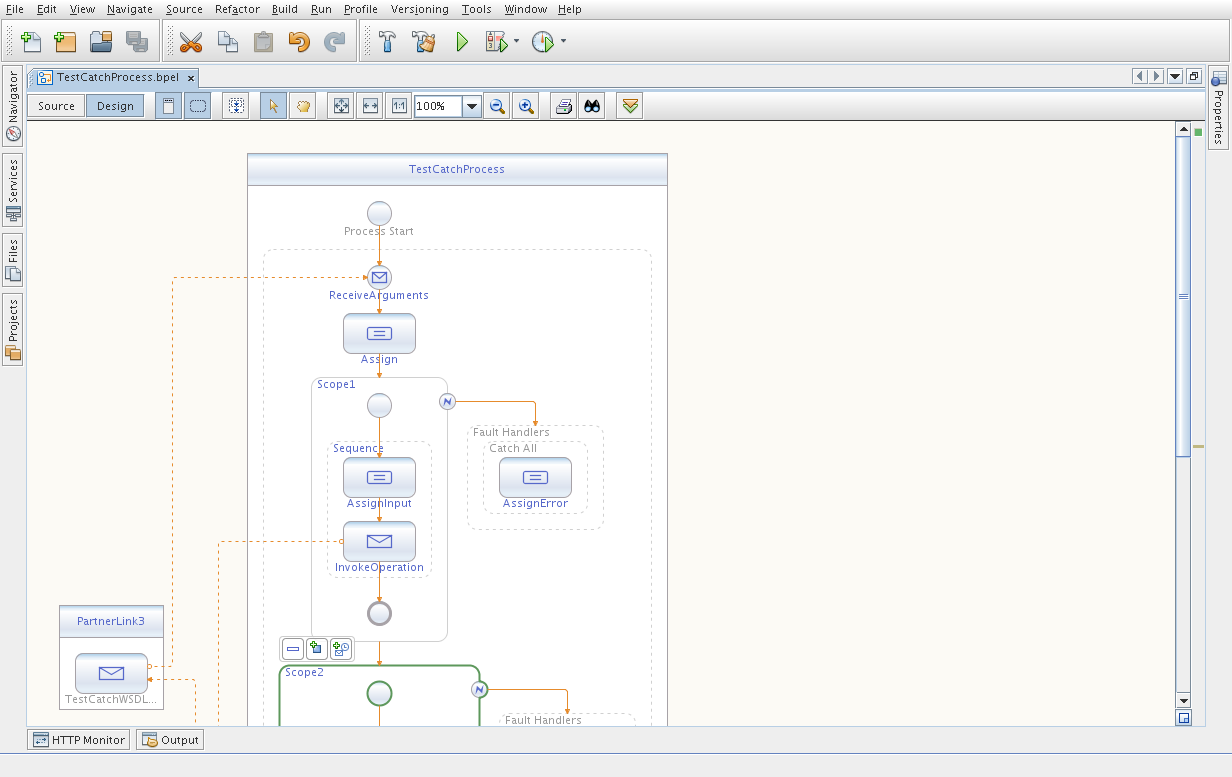
\includegraphics[width=12cm,height=8cm,bb=0 0 1232 777]{chapter1/bpel_des.png}
 % bpel_des.png: 1232x777 pixel, 72dpi, 43.47x27.42 cm, bb=0 0 1232 777
 \caption{Pakiet Netbeans - wizualny edytor procesu BPEL}
 \label{fig:bpel_sample_des}
\end{figure}

Istnieje r�wnie� szereg narz�dzi u�atwiaj�cych modelowanie proces�w w j�zyku BPEL, takich jak oparte na platformie Eclipse Oracle BPEL Designer\cite{bpel:tool:oracle} i IBM Websphere Application Developer Integration Edition\cite{bpel:tool:websphere}, czy wybrany przez autor�w, oparty o platform� Netbeans BPEL Designer\cite{bpel:tool:netbeans} (przedstawiony na rys. \ref{fig:bpel_sample_des}). Wyb�r ten zosta� podyktowany dojrza�o�ci� i otwarto�ci� rozwi�zania, oraz zaawansowan� integracj� z wybranym wcze�niej �rodowiskiem OpenESB.


\newpage

Wysoka innowacyjno�� opisanych w niniejszym rozdziale koncepcji i technologii, sprawia �e nie s� one obecnie w powszechnym u�yciu.
% Opisane w niniejszym rozdziale koncepcje i technologie stanowi� innowacyjne rozwi�zania, nie b�d�ce jeszcze w powszechnym u�yciu w �wiecie oprogramowania du�ej skali.
Wydajno�� aplikacji zrealizowanych z ich u�yciem, mo�e by� badana z u�yciem oprogramowania stworzonego w ramach niniejszej pracy.
% Aplikacje stworzone z ich pomoc� s� przedmiotem test�w stworzonego w ramach pracy oprogramowania.

%\part{Implementacja}

\chapter{System badania wydajno�ci}

W rozdziale tym opisane zosta�y kryteria jakie powinien spe�nia� system wspomagaj�cy badanie wydajno�ci system�w o architekturze SOA. W kolejnych punktach rozdzia�u przedstawiono analiz� w kontek�cie tych kryteri�w oraz uzasadnienie ostatecznego wyboru.
% W dalszej cz�ci znajdzie si� analiza mo�liwych rozwi�za� w kontek�cie tych kryteri�w, oraz wyja�nienie ostatecznego wyboru.


W celu zbadania wydajno�ci aplikacji zbudowanej zgodnie z paradygmatem SOA potrzebne s� dodatkowe dane zbierane w trakcie dzia�ania takiej aplikacji. Dane te opisuj� jednostkowe operacje wykonywane przez aplikacj� (np. wywo�anie us�ugi webservice, sekwencje wywo�a� operacji, p�tle, instrukcje warunkowe, bloki obs�ugi wyj�tk�w) i zawieraj� m.in. informacj� o czasie trwania danej operacji, dodatkowych parametrach (np. adres i operacja przy us�udze webservice), statusie (np. zako�czenie poprawne, zako�czenie z powodu wyj�tku) itp. Po zebraniu pomiary mog� zosta� przedstawione u�ytkownikowi w czytelny spos�b, np. jako diagramy Gantta\cite{diagram:gantt}, model BPEL, wykresy, itp.

W systemach badaj�cych wydajno�� za zbieranie danych odpowiada sensor wydajno�ci.
Mo�na wyr�ni� dwa podej�cia do kwestii jego lokalizacji:
\begin{itemize}
 \item Umieszczenie sensora wydajno�ci w \textbf{obr�bie us�ug}.  Takie podej�cie wymaga modyfikacji ka�dej z us�ug, co powoduje, �e us�ugi musz� by� �wiadome brania udzia�u w badaniu wydajno�ci. W przypadku posiadania kodu �r�d�owego us�ug konieczna jest jego analiza i odpowiednia modyfikacja, co czyni ten proces czasoch�onnym; przy braku kodu �r�d�owego us�ug odpowiednia modyfikacja jest ju� cz�sto niewykonalna w rozs�dnych granicach czasowych. 
 \item Umieszczenie sensora wydajno�ci w \textbf{obr�bie kontenera}. Zalet� tego podej�cia jest fakt, �e modyfikacje �rodowiska w kt�rym dzia�aj� us�ugi nale�y wykona� tylko raz, niezale�nie od ilo�ci wykorzystywanych us�ug.
\end{itemize}
Wariant z sensorem wydajno�ci w us�ugach jest niepraktyczny w realizacji i jako taki zosta� odrzucony.  Podj�to decyzj� o umieszczeniu sensora wydajno�ci w obr�bie kontenera szyny ��cz�cej us�ugi. Zarys koncepcji badania wydajno�ci aplikacji zosta� przedstawiony na rysunku \ref{fig:desc:arch}.

\begin{figure}
 \centering
 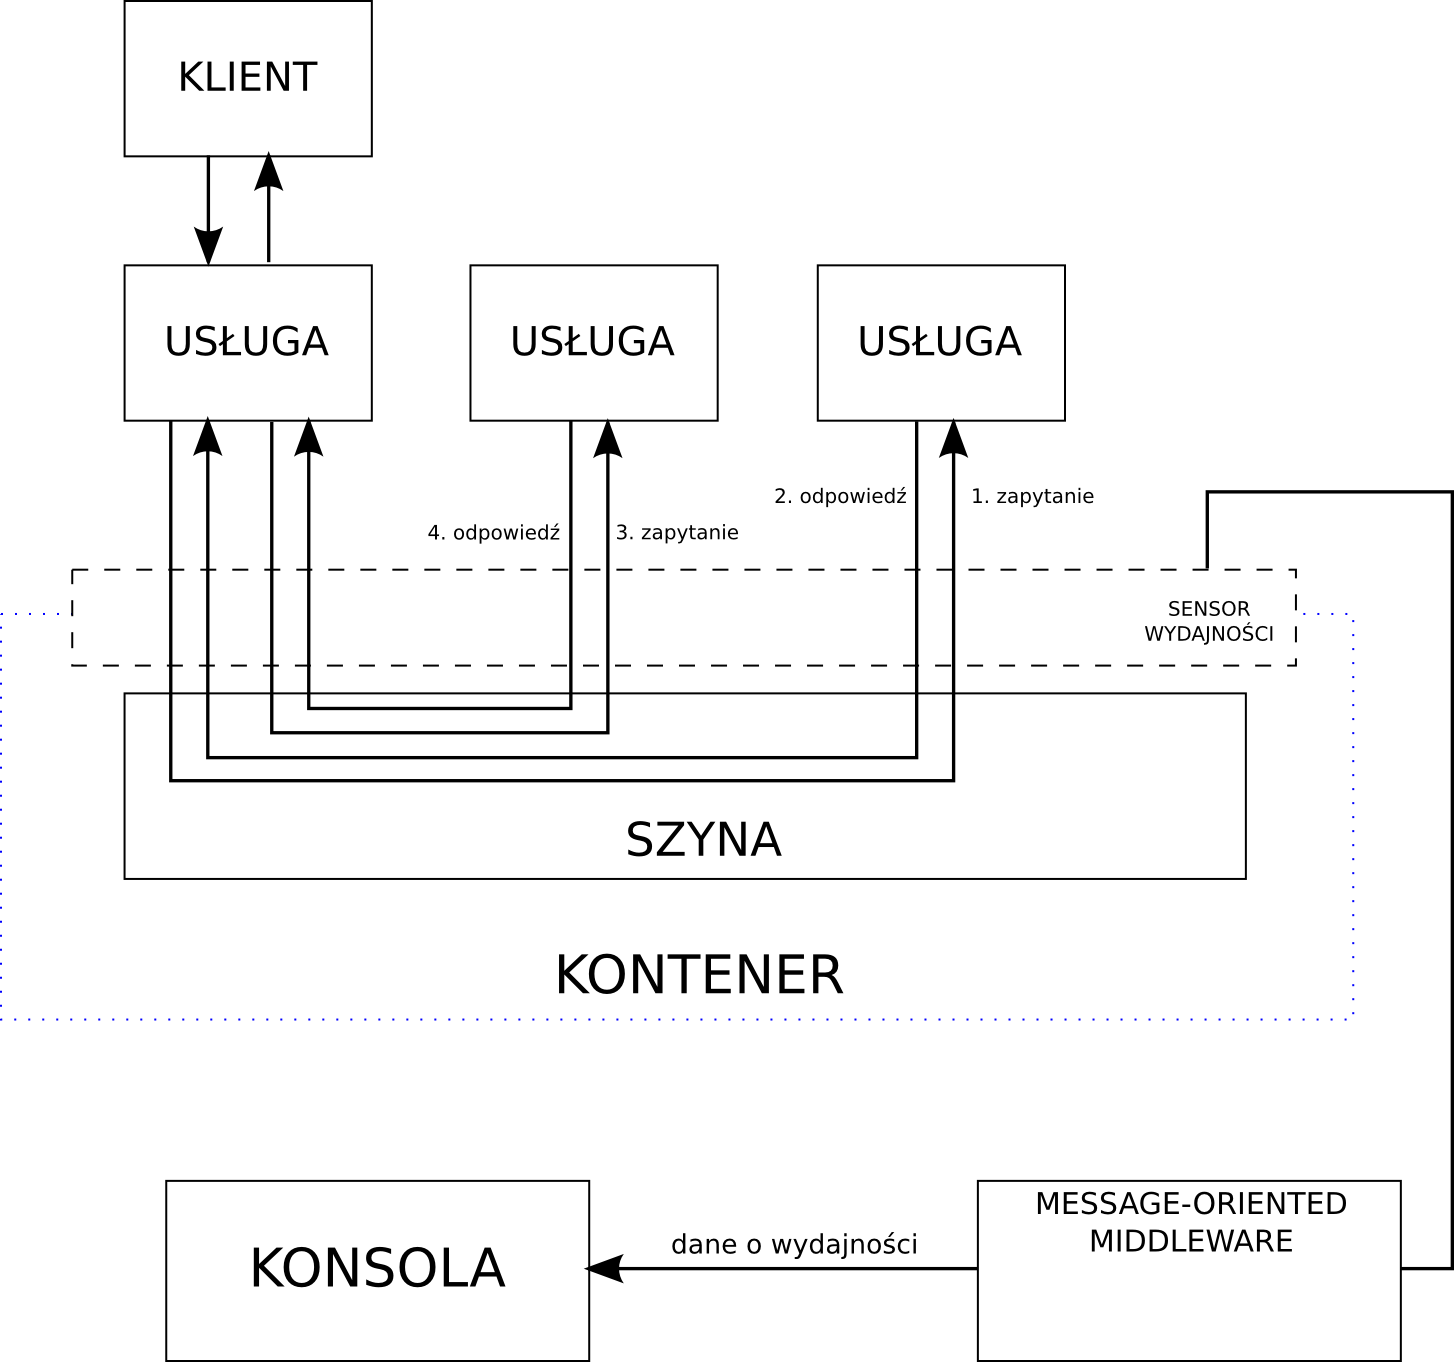
\includegraphics[bb=0 0 349 327]{description/esb2-eff.png}
 % esb2-eff.png: 911x853 pixel, 188dpi, 12.31x11.52 cm, bb=0 0 349 327
 \caption{Architektura u�ywana do badania wydajno�ci aplikacji}
 \label{fig:desc:arch}
\end{figure}


Przedstawiona og�lna architektura systemu badania wydajno�ci aplikacji opartych o paradygmat SOA ukrywa w sobie szereg problem�w i decyzji, zar�wno koncepcyjnych (np. spos�b dzia�ania sensora wydajno�ci, spos�b identyfikacji proces�w i aktywno�ci badanej us�ugi) jak i technologicznych (np. rodzaj rozwi�zania MOM u�ywanego do przesy�ania danych o wydajno�ci). Prowadzi to do istnienia wielu mo�liwych sposob�w realizacji takiej aplikacji. Przed wybraniem jednego sposobu 
% badania wydajno�ci - kt�re zostanie zaimplementowane i przetestowane w oparciu o przyk�adowe aplikacje - 
nale�a�o zdefiniowa� kryteria r�nicuj�ce potencjalne rozwi�zania. Kryteriami tymi s� wymagania funkcjonalne i niefunkcjonalne w stosunku do element�w architektury zawartych na rysunku \ref{fig:desc:arch}.

\section{Wymagania}

Zestaw wymaga� zosta� podzielony na dwie grupy, pierwsza dotyczy konsoli wizualizacyjnej, a druga sensora wydajno�ci.

\subsection{Wymagania w stosunku do konsoli}

W stosunku do konsoli wizualizacyjnej postawiono nast�puj�ce wymagania:

\begin{itemize}
 \item przygotowanie �rodowiska poprzez dodanie sensora wydajno�ci (mo�e si� to wi�za� z np. instrumentacj� bibliotek serwera, modyfikacj� jego plik�w startowych lub rozmieszczeniem (ang. deploy) w serwerze specjalnej aplikacji monitoruj�cej wydajno��)
 \item odbieranie informacji o wydajno�ci z wykorzystaniem Message Oriented Middleware (np. JMS)
 \item obrazowanie na bie��co (ang. online) wynik�w badania wydajno�ci aplikacji
 \item prezentacja wynik�w w postaci sekwencji j�zyka BPEL (np. wykonanie operacji us�ugi webservice, przypisanie warto�ci do zmiennej)
 \item r�wnoczesna obs�uga kilku instancji �rodowiska ESB
\end{itemize}

Uzyskiwane dane o wydajno�ci aplikacji powinny by� przedstawiane w spos�b przejrzysty dla u�ytkownika w postaci diagramu z modelem BPEL. Dla ka�dej operacji przedstawionej na diagramie powinny by� dost�pne informacje:
\begin{itemize}
 \item �redni, minimalny, maksymalny oraz sumaryczny czas trwania operacji
 \item czas rozpocz�cia i zako�czenia, parametry, rezultat (np. zako�czenie przez rzucenie wyj�tku) ka�dego wywo�ania operacji.
\end{itemize}

\subsection{Wymagania w stosunku do sensora wydajno�ci}

Typowa metryka uzyskiwana z procesu mierzenia wydajno�ci - czas wykonania operacji - mo�e mie� r�n� warto�� w zale�no�ci od warstwy na kt�rej dzia�a sensor wydajno�ci. Sytuacj� t� przedstawiono na rysunku \ref{fig:desc:invoke}, na kt�rym znajduje si� przyk�adowy schemat wywo�ania us�ugi webservice z poziomu j�zyka BPEL w OpenESB. Przyk�adowo, je�li sensor umie�cimy w obr�bie JBI, to w zmierzonym czasie wykonania operacji webservice b�dzie zawarta tylko cz�� 4 i 5 sekwencji rzeczywistego wywo�ania operacji (por. rysunek \ref{fig:desc:invoke}). Pomini�ty zostanie w�wczas wp�yw adaptera JBI oraz silnika BPEL na czas wykonania operacji, a tym samym zaburzony zostanie wynik badania wydajno�ci aplikacji. W celu zniwelowania skutk�w niew�a�ciwego zbierania wynik�w wydajno�ci, nale�y sensor wydajno�ci umie�ci� w obr�bie silnika BPEL. 

\begin{figure}[h!kp]
 \centering
 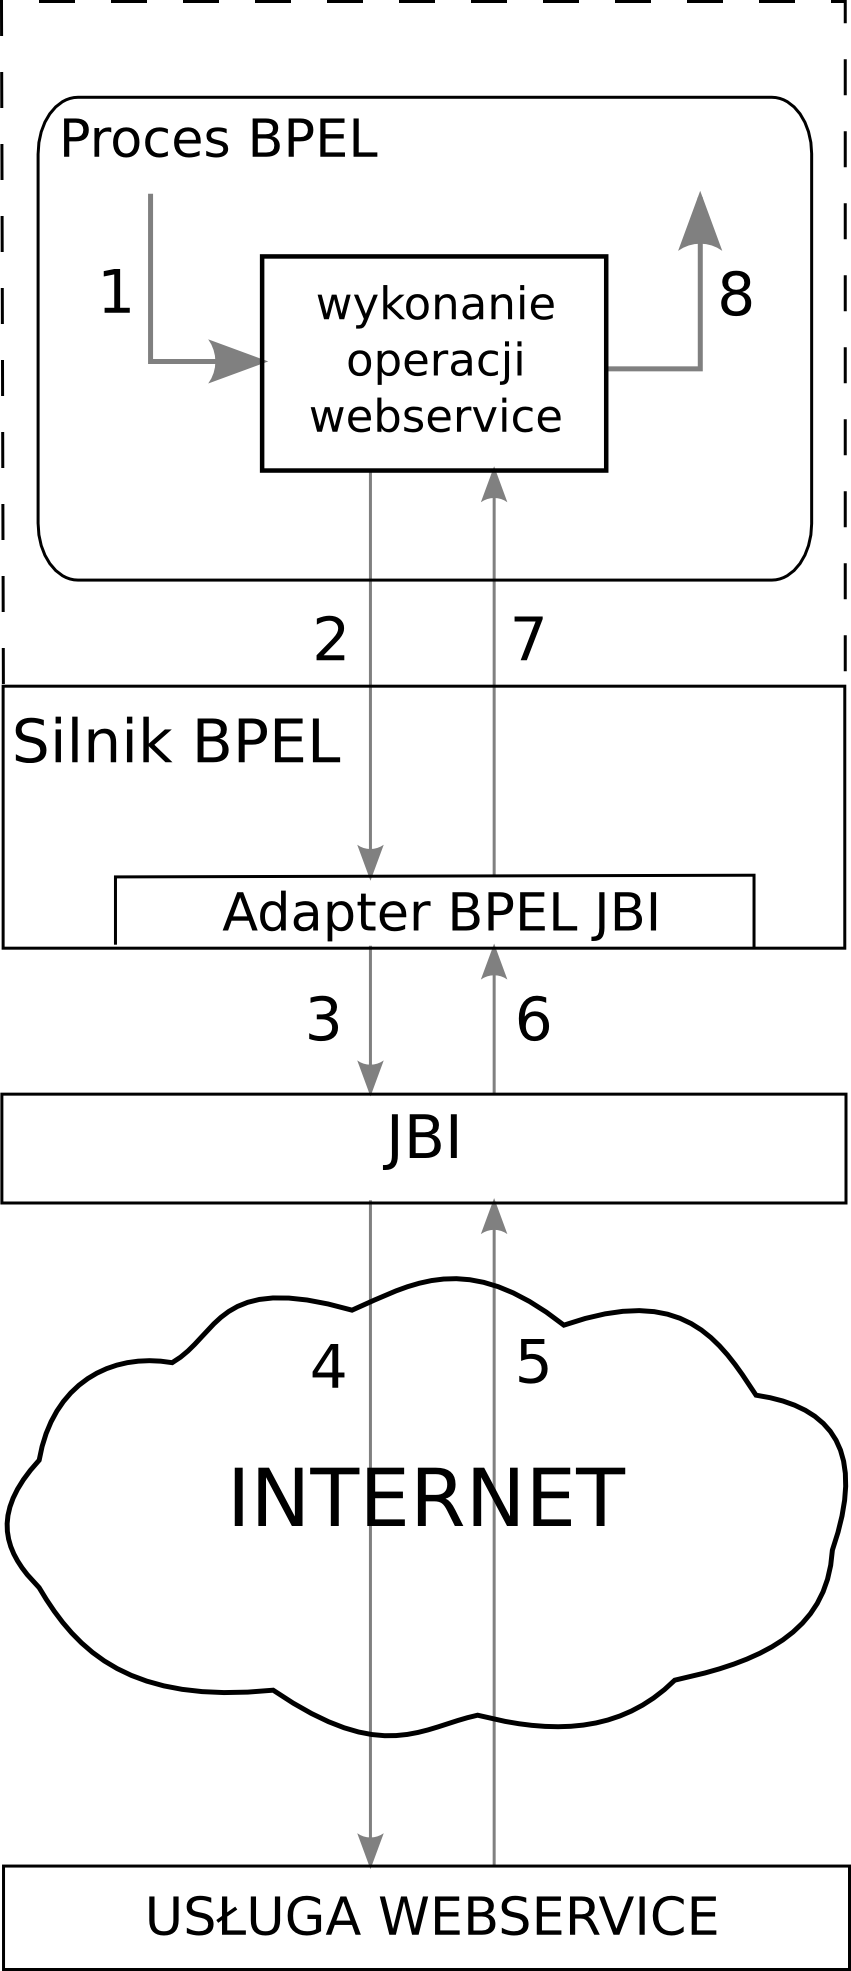
\includegraphics[bb=0 0 204 473]{description/arch3.png}
 % arch3.png: 533x1235 pixel, 188dpi, 7.20x16.68 cm, bb=0 0 204 473
 \caption{Schemat wywo�ania us�ugi webservice w OpenESB}
 \label{fig:desc:invoke}
\end{figure}

Wymagania w stosunku do sensora wydajno�ci:
\begin{itemize}
 \item dzia�anie mo�liwie blisko silnika BPEL, w celu uzyskania dok�adnych wynik�w
 \item brak ingerencji w zewn�trzne us�ugi (sensor nie mo�e modyfikowa� sposobu ich dzia�ania)
 \item minimalny wp�yw na dzia�anie aplikacji (najwa�niejsze jest ograniczenie narzut�w czasowych zwi�zanych ze zbieraniem danych o wydajno�ci)
 \item mo�liwo�� implementacji w najpopularniejszych serwerach aplikacji (sama implementacja sensora wydajno�ci b�dzie r�ni�a si� szczeg�ami w zale�no�ci od serwera aplikacji)
 \item zautomatyzowany proces do��czania sensora wydajno�ci, z minimaln� ingerencj� u�ytkownika.
% - kwestia u�ycia tego powinna by� w miar� niezale�na od JBI/ESB
\end{itemize}





\section{Koncepcje rozwi�za�}

W trakcie analizy mo�liwo�ci podej�cia do postawionego wcze�niej problemu, rozr�nione zosta�y dwie grupy rozwi�za�:
\begin{itemize}
 \item Nie wymagaj�ce modyfikacji kodu - koncepcje opieraj�ce si� na wykorzystaniu ju� istniej�cych mo�liwo�ci pobrania informacji pomiarowych ze �rodowiska ESB
 \item Wymagaj�ce modyfikacji �rodowiska testowego - koncepcje, kt�rych wykorzystanie opiera si� na zmianach w kodzie aplikacji, b�d� �rodowiska
\end{itemize}


\subsection{Koncepcje nie wymagaj�ce modyfikacji kodu BPEL}

\subsubsection{Interfejs monitorowania BPEL OpenESB}
Silnik us�ugowy BPEL zastosowany w implementacji OpenESB udost�pnia interfejs programistyczny pozwalaj�cy na monitorowanie i zarz�dzanie procesami wykonywanymi w jego obr�bie. Do jego mo�liwo�ci nale�� mi�dzy innymi:
\begin{itemize}
 \item Udost�pnianie identyfikator�w proces�w oraz ich instancji
 \item Zarz�dzanie cyklem �ycia proces�w oraz ich instancji
 \item Udost�pnianie informacji o b��dach, kt�re wyst�pi�y w instancjach proces�w
 \item Dost�p i zmiana zmiennych instancji
 \item Dost�p do informacji na temat proces�w, instancji, a tak�e aktywno�ci instancji (activity)
\end{itemize}

Wymieniony jako ostatni dost�p do informacji na temat aktywno�ci instancji pozwala na sprawdzenie takich danych jak:
\begin{itemize}
 \item Status aktywno�ci
 \item Znacznik czasowy pocz�tku i ko�ca aktywno�ci
 \item Czas trwania 
 \item Numer iteracji (p�tli)
\end{itemize}

\paragraph{Spos�b dost�pu}
\begin{figure}[h!]
 \centering
 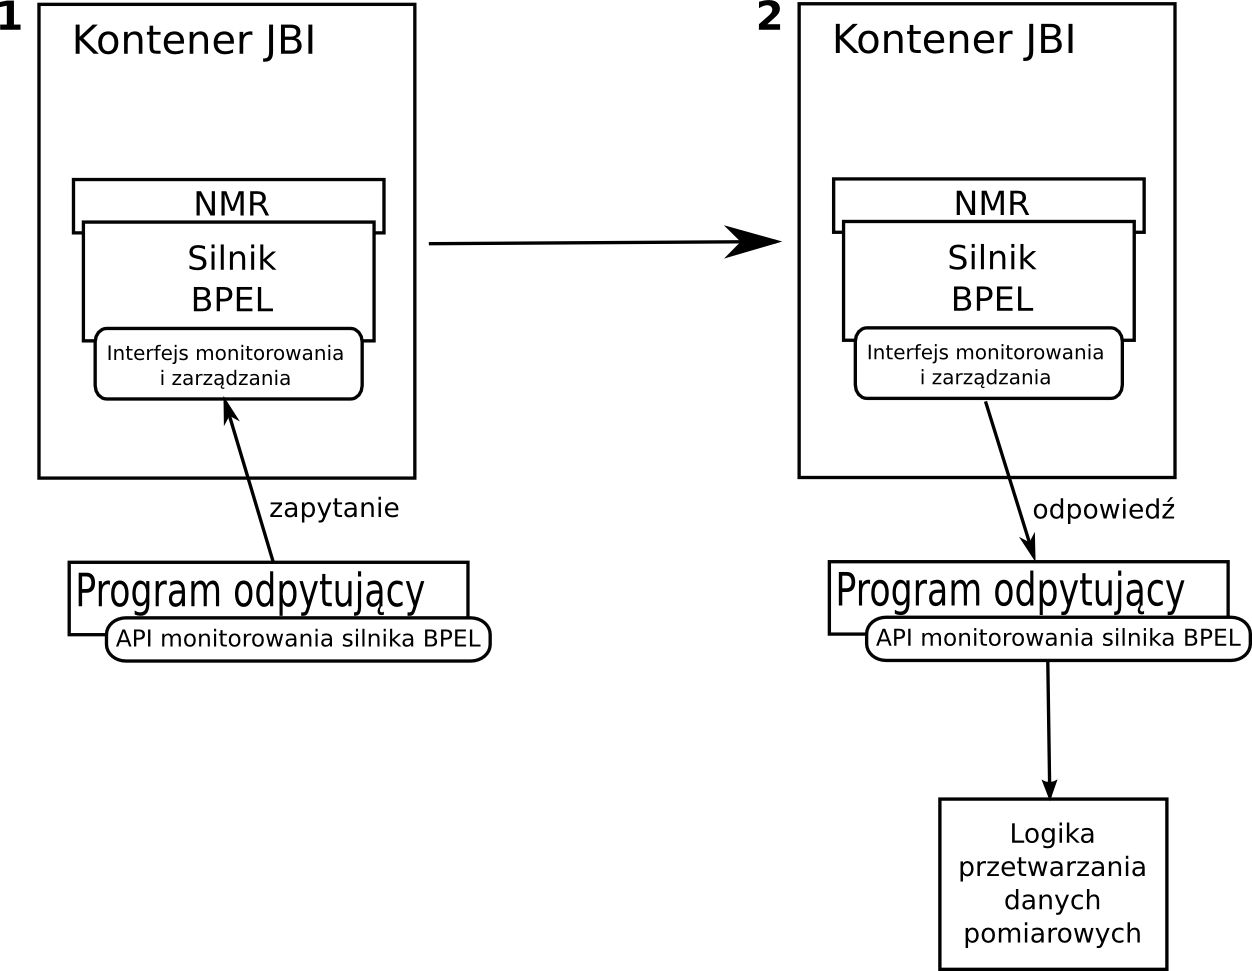
\includegraphics[bb=0 0 301 233]{description/bpel_monitoring_concept.png}
 % bpel_monitoring_concept.png: 303x197 pixel, 94dpi, 8.20x5.33 cm, bb=0 0 232 151
 \caption{Koncepcja rozwi�zania w oparciu o interfejs monitorowania silnika BPEL}
 \label{fig:bpel_monitoring_concept}
\end{figure}

Rysunek \ref{fig:bpel_monitoring_concept} przedstawia ide� rozwi�zania. Bazuje ona na aktywnym, synchronicznym odpytywaniu o dane pomiarowe.

\paragraph{Analiza trafno�ci rozwi�zania}
Odpowiednie u�ycie i agregacja danych pozwala�oby na stworzenie zak�adanego systemu do pomiar�w wydajno�ci. Rozwi�zanie to ma jednak jedn� zasadnicz� wad� - dane z interfejsu zbierane s� synchronicznie\footnote{u�yty zosta� tutaj wzorzec Wizytora\cite{concept:gang_of_four}}, co poci�ga za sob� konsekwencje w postaci mo�liwo�ci utraty cz�ci danych - problem ten dotyczy przede wszystkim konstrukcji p�tli. Problemem by�aby r�wnie� agregacja otrzymanych w taki spos�b danych oraz dob�r cz�sto�ci pr�bkowania (w zale�no�ci od dobranej warto�ci stworzone narz�dzie by�oby albo nara�one na utrat� danych, albo na du�y nak�ad oblicze� potrzebny do agregacji).

\subsubsection{HULP}
HULP to biblioteka dla j�zyka Java\texttrademark pozwalaj�ca na zinstrumentowanie kodu  celem dokonywania pomiar�w czasu wykonania obszar�w kodu. Oferuje ona prosty interfejs programistyczny, z kt�rego u�yciem mo�liwe jest zaznaczanie pocz�tku i ko�ca wykonania obszaru kodu. Wykonane w taki spos�b pomiary s� nast�pnie zbierane, agregowane i prezentowane z pomoc� aplikacji WWW.

\paragraph{Cechy rozwi�zania}
\begin{itemize}
 \item Prosta w realizacji instrumentacja. Przyk�adowo:
 
\begin{lstlisting}[frame=tb]
  ...
  public void komenda(String parameter) {
    Measurement m = Measurement.begin("komenda", parameter);
    try {
       ... badany obszar kodu
    } finally {
       m.end();
    }
  }
\end{lstlisting}
 \item Niski narzut czasowy zinstrumentowanego kodu przy wy��czonym zbieraniu
  danych
 \item Nieskomplikowana budowa - HULP sk�ada si� z trzech komponent�w:
  interfejs instrumentacji, klasy agregacji i servlet odpowiedzialny za
  prezentacje wynik�w
 \item Zagregowane wyniki zwracane s� w postaci zestawu nast�puj�cych danych:
 \begin{itemize}
    \item ilo�ci wywo�a�
    \item czas trwania pomiar�w\footnote{od pierwszego begin() do ostatniego end()}
    \item sumy oraz �redniej czasu sp�dzonego w zinstrumentowanych obszarach kodu
    \item przepustowo�ci\footnote{ilo�� wywo�a� podzielona przez czas trwania
     pomiar�w} pomiaru
    \item obci��enia\footnote{suma czasu sp�dzonego w zinstrumentowanych obszarach kodu podzielona przez czas trwania pomiar�w} generowanego podczas pomiaru
 \end{itemize}
\end{itemize}

\paragraph{Idea rozwi�zania z u�yciem HULP}
Rozwa�anie u�ycia HULP opiera si� na fakcie, i� kod OpenESB ju� zosta� zinstrumentowany z pomoc� tej biblioteki. Idea rozwi�zania opiera si� na pobieraniu danych z warstwy prezentacji HULP (servletu), dla ich dalszej analizy (og�lny schemat koncepcji przedstawia rys. \ref{fig:hulp_concept}).

\begin{figure}[h!]
 \centering
 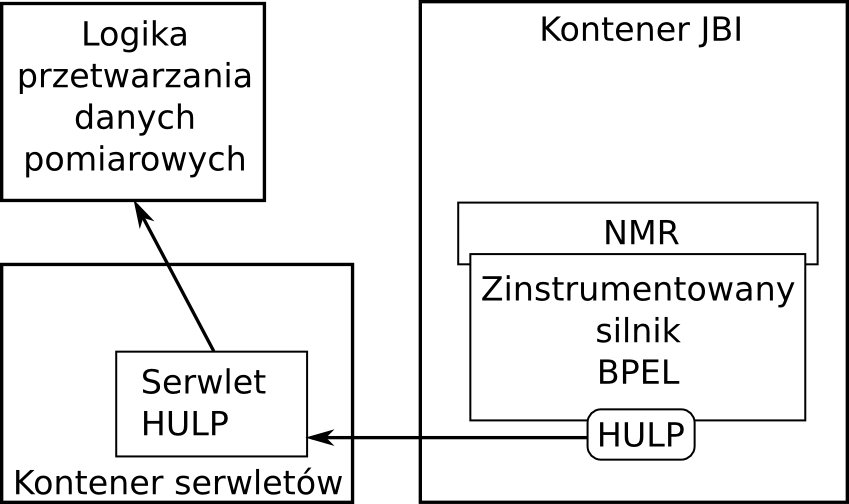
\includegraphics[bb=0 0 202 115]{description/hulp_concept.png}
 % hulp_concept.png: 264x150 pixel, 94dpi, 7.14x4.06 cm, bb=0 0 202 115
 \caption{Koncepcja rozwi�zania z u�yciem HULP}
 \label{fig:hulp_concept}
\end{figure}


\paragraph{Analiza trafno�ci rozwi�zania}
Pomimo szeregu zalet tego rozwi�zania nie spe�nia ono za�o�e� postawionych na pocz�tku tego rozdzia�u. Do najwa�niejszych problem�w zwi�zanych z u�yciem HULP nale��:
\begin{itemize}
 \item konieczno�� modyfikacji kodu OpenESB (poniewa� nie wszystkie interesuj�ce z punktu widzenia pracy obszary kodu zosta�y zinstrumentowane)
 \item brak znacznik�w czasowych
 \item trudno�ci w identyfikacji badanych proces�w biznesowych\footnote{trudno�ci w odr�nieniu kilku dzia�aj�cych jednocze�nie proces�w biznesowych}
 \item niepe�no�� zagregowanych danych
 \item trudny do interpretacji maszynowej format dostarczanych danych.
\end{itemize}

\subsection{Obserwator zdarze� silnika BPEL}
Silnik BPEL OpenESB udost�pnia interfejs (BPEL SE Events Listener) pozwalaj�cy na zarejestrowanie obserwator�w\cite{concept:gang_of_four} zachodz�cych w nim zdarze�. Pozwala to na odbieranie informacji dotycz�cych proces�w oraz ich aktywno�ci i warto�ci zadeklarowanych w nich zmiennych.\cite{concept:bpel_events_listener}

Do monitorowanych zdarze� nale��: 
\begin{itemize}
 \item pocz�tek, koniec, u�pienie i wybudzenie \textbf{procesu}
 \item pocz�tek, koniec i b��d \textbf{sk�adowej procesu}
 \item zmiany warto�ci \textbf{zmiennych procesu}
\end{itemize}

Ka�de otrzymywane zdarzenie jest opatrzone identyfikatorem procesu i instancji oraz znacznikiem czasowym. Zdarzenia dotycz�ce aktywno�ci procesu zawieraj� wyra�enie XPath prowadz�ce do tej aktywno�ci.

Klasa obserwatora powinna implementowa� nast�puj�cy interfejs:

\begin{lstlisting}[frame=tb]
 interface EventListener {
    void processEvent(Event event);
 }
\end{lstlisting}

\paragraph{Idea rozwi�zania}

\begin{figure}[h!]
 \centering
 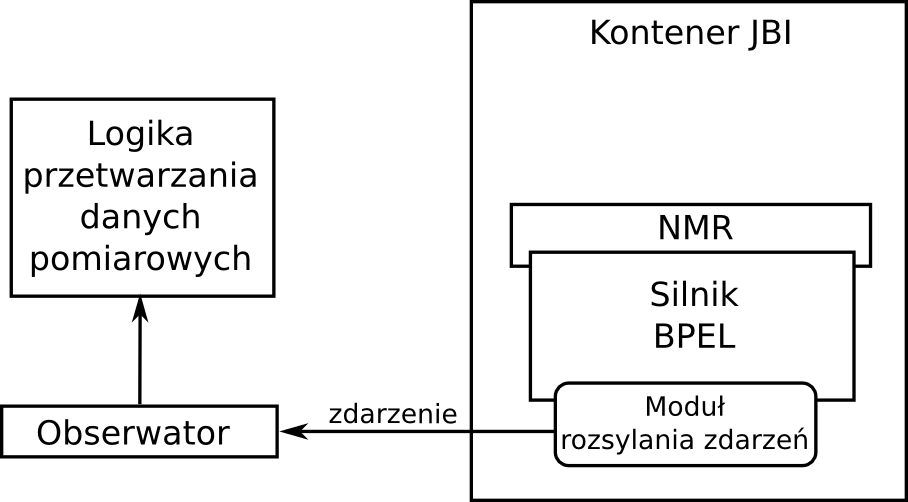
\includegraphics[bb=0 0 225 133]{description/listener_concept.png}
 % listener_concept.png: 294x173 pixel, 94dpi, 7.95x4.68 cm, bb=0 0 225 133
 \caption{Koncepcja rozwi�zania z u�yciem BPEL SE Events Listener}
 \label{fig:listener_concept}
\end{figure}

Rysunek \ref{fig:listener_concept} przedstawia ide� rozwi�zania opartego o BPEL SE Events Listener. Logika przetwarzania danych pomiarowych otrzymywa�aby dane po uprzednim zarejestrowaniu obserwatora zdarze� w silniku BPEL.

\paragraph{Analiza trafno�ci rozwi�zania}
Rozwi�zanie oparte o BPEL SE Events Listener posiada wiele zalet, takich jak prostota, asynchroniczny model dzia�ania oraz du�y zakres dostarczanych danych. Wa�na w�a�ciwo�ci� jest r�wnie� oparty o pul� w�tk�w nieblokuj�cy model rozsy�ania zdarze� do obserwator�w, znacznie zmniejszaj�cy narzuty czasowe z nim zwi�zane. Rozwi�zanie nie spe�nia postawionych za�o�e� pracy: do jego pe�nego dzia�ania konieczna jest instrumentacja aplikacji umieszczanej na serwerze\footnote{konieczne jest dodanie do niej implementacji obserwatora oraz dopisanie nazwy jego klasy w pliku \nolinebreak{META-INF/services/com.sun.jbi.engine.bpel.core.bpel.event.BPELEventListener}}. Niew�tpliwym problemem jest r�wnie� brak przeno�no�ci tego rozwi�zania\footnote{Pozwala�oby ono na monitorowanie jedynie tego konkretnego silnika BPEL} do innych �rodowisk ESB.

\subsection{Koncepcje wymagaj�ce instrumentacji kodu BPEL}

\subsubsection{Modyfikacja kodu aplikacji}

Najprostszym rozwa�anym rozwi�zaniem jest zmodyfikowanie kodu testowanej aplikacji w taki spos�b aby sama dostarcza�a informacji pomiarowych. Modyfikacja taka opiera�aby si� na dodaniu takiej logiki do kodu BPEL w formie odpowiednio umieszczonych operacji Invoke, przed ka�d� mo�liw� operacj�. Operacje te wysy�a�yby informacje pomiarowe do uprzednio stworzonej us�ugi monitoruj�cej.
Koncepcj� t� ukazuje rysunek 3.6.

\begin{figure}[htp!]
 \centering
 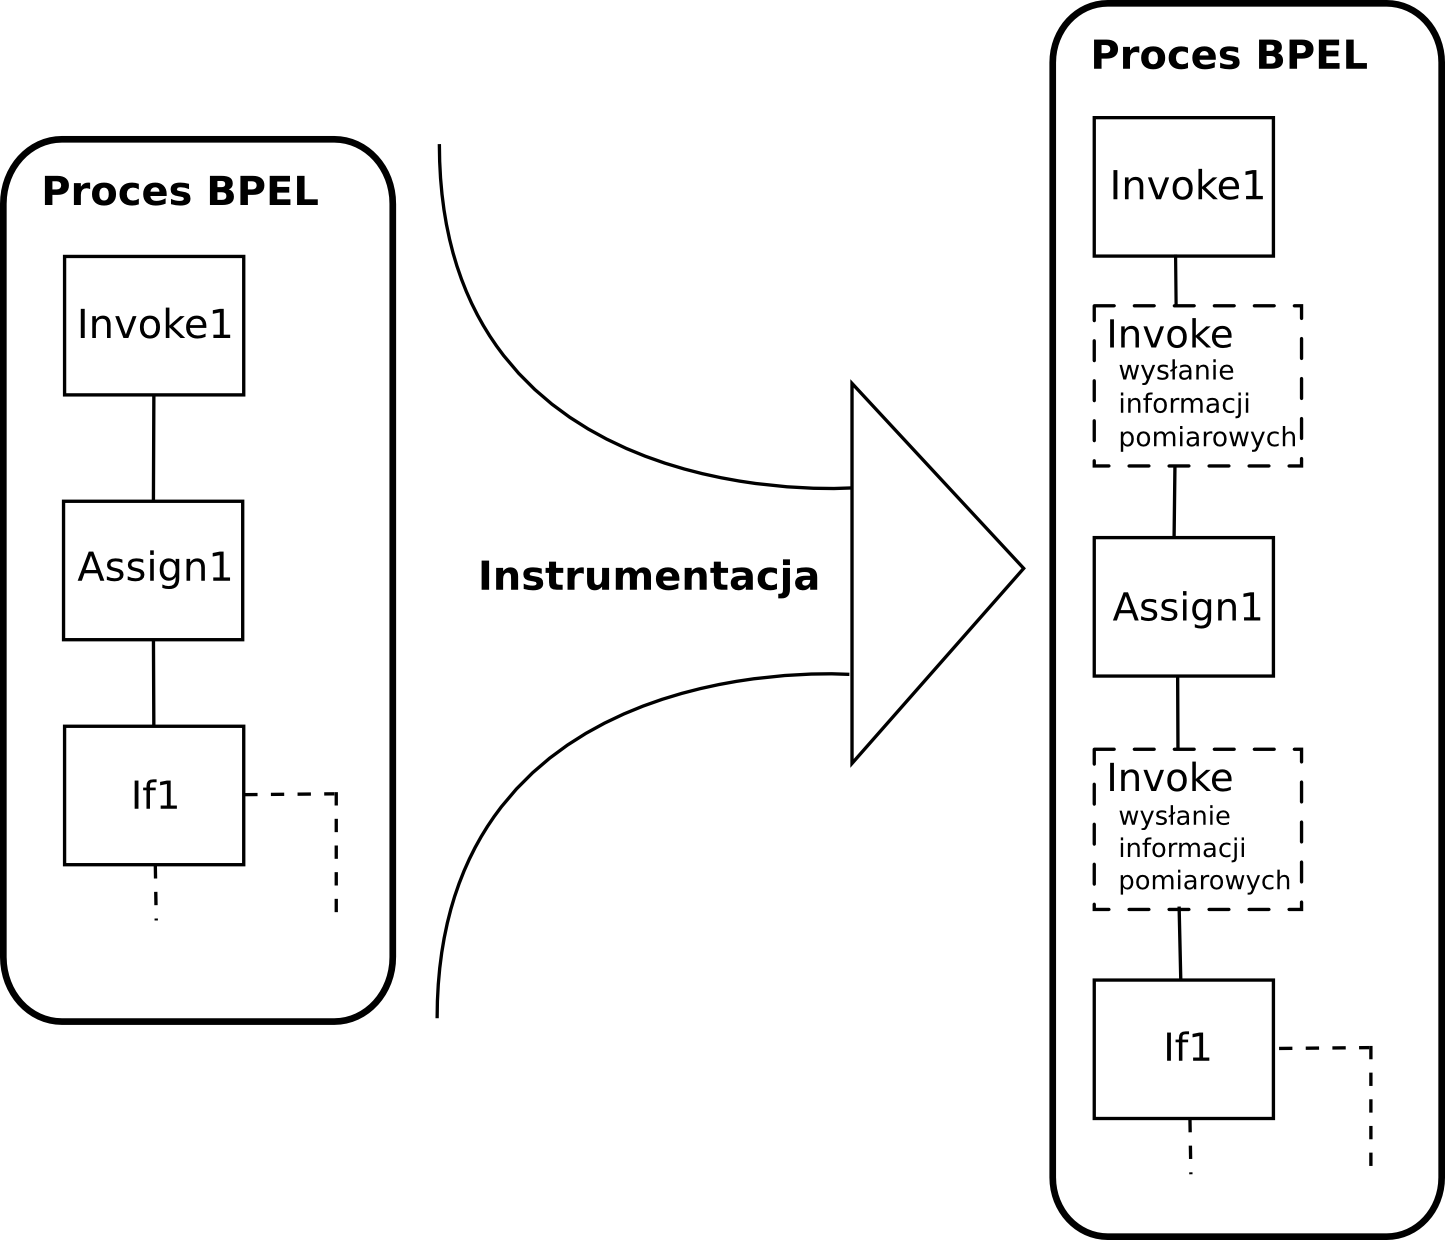
\includegraphics[bb=0 0 295 255]{description/bpel_code_instrumenation_concept.png}
 % bpel_code_instrumenation_concept.png: 385x332 pixel, 94dpi, 10.42x8.98 cm, bb=0 0 295 255
 \label{fig:bpel_code_instrumentation_concept}
 \caption{Koncepcja instrumentacji kodu BPEL aplikacji}
\end{figure}

Trudno�ci w realizacji tego rozwi�zania, konieczno�� modyfikacji ju� zbudowanej aplikacji oraz niska wiarygodno�� dostarczanych znacznik�w czasowych wyklucza jego praktyczne zastosowanie.

\subsubsection{Modyfikacja kodu �rodowiska wykonawczego}
Skomplikowanym, ale jednocze�nie posiadaj�cym najwi�cej mo�liwo�ci rozwi�zaniem jest zmodyfikowanie �rodowiska wykonawczego w taki spos�b, aby generowa�o ono zdarzenia i  przekazywa�o je asynchronicznie do zbiorczego punktu celem dalszej analizy. Zdarzenia te przenosi�yby ze sob� nast�puj�ce informacje:
\begin{itemize}
 \item znaczniki czasowe operacji
 \item szereg jednoznacznych identyfikator�w pozwalaj�cych okre�li� pochodzenie danych
 \begin{itemize}
  \item identyfikator procesu BPEL
  \item identyfikator instancji procesu
  \item identyfikator aktywno�ci procesu
  \item identyfikator w�tku
 \end{itemize}
 \item typ aktywno�ci i informacje jej dotycz�ce (tj. np. identyfikator wywo�ywanej us�ugi w aktywno�ci Invoke)
\end{itemize}

Generowanie by�oby wyzwalane nast�puj�cymi zdarzeniami:
\begin{itemize}
 \item rozpocz�cie procesu biznesowego,
 \item rozpocz�cie aktywno�ci procesu,
 \item rzucenie wyj�tku w aktywno�ci,
 \item zako�czenie aktywno�ci procesu,
 \item zako�czenie procesu biznesowego.
\end{itemize}

Asynchronicznie generowane zdarzenia mog� by� przekazywane bezpo�rednio do punktu zbiorczego. Celem polepszenia skalowalno�ci rozwi�zania mo�na publikowa� zdarzenia z u�yciem oprogramowania realizuj�cego koncepcj� MOM (np. JMS).

Rysunek \ref{fig:bpel_engine_instrumentation_concept} przedstawia zarys tej koncepcji. Wynika z niego, �e aby dokona� takiej instrumentacji konieczna jest statyczna modyfikacja kodu silnika BPEL. Mo�na tego dokona� albo modyfikuj�c jego otwarty kod �r�d�owy, lub u�y� narz�dzia do instrumentacji kodu wykonawczego.

\begin{figure}[h!]
 \centering
 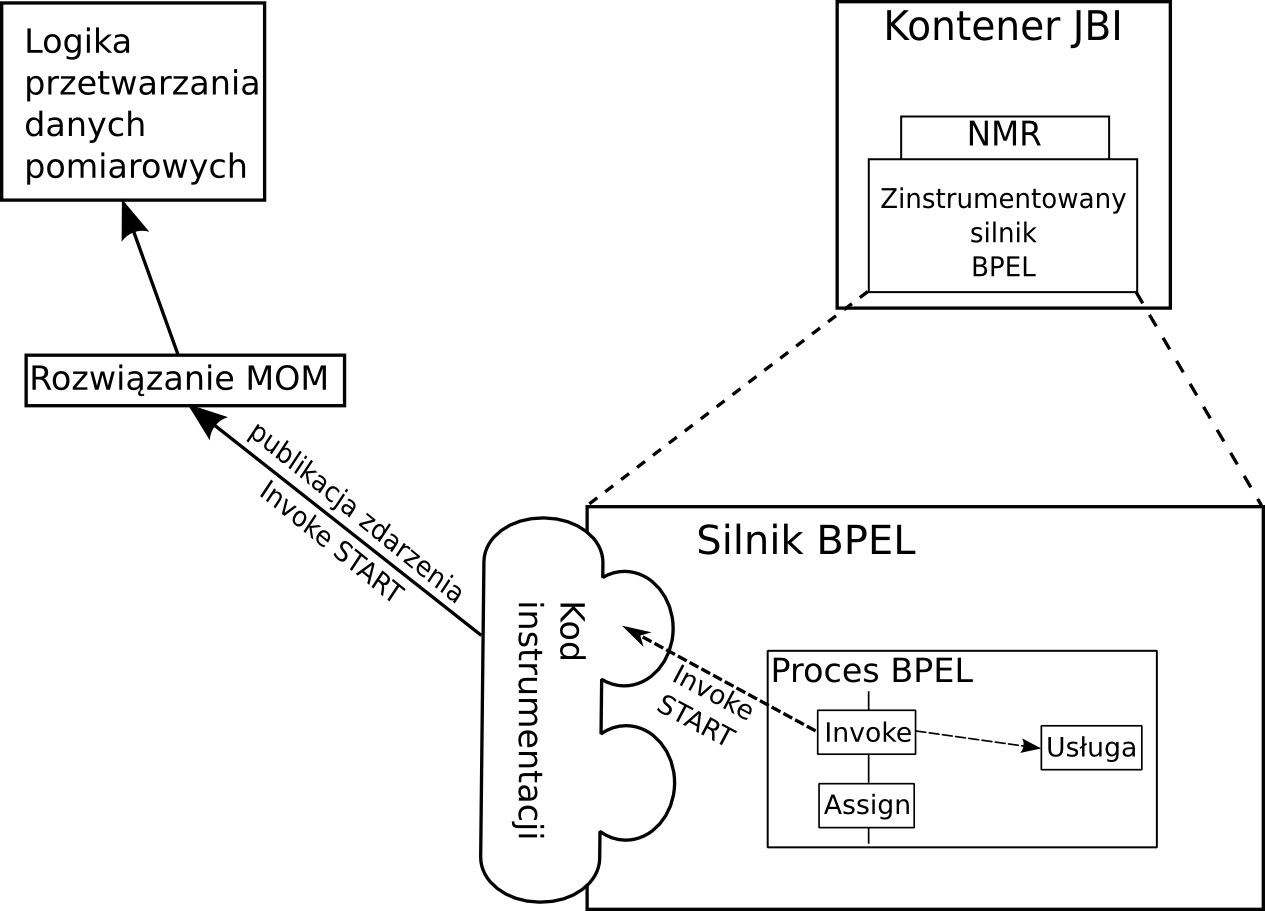
\includegraphics[bb=0 0 304 219]{description/bpel_engine_instrumentation_concept.png}
 % bpel_engine_instrumentation_concept.png: 396x285 pixel, 94dpi, 10.71x7.71 cm, bb=0 0 304 219
 \caption{Koncepcja instrumentacji �rodowiska wykonania}
 \label{fig:bpel_engine_instrumentation_concept}
\end{figure}

\subsubsection{Analiza trafno�ci rozwi�zania}
Brak konieczno�ci modyfikacji kodu �r�d�owego zar�wno aplikacji, jak i �rodowiska, jest bardzo du�� zalet� tego rozwi�zania. Drug� zalet� jest wiarygodno�� dostarczanych danych - instrumentacja kodu w odpowiednio dobranych punktach niweluje problem niemiarodajnych znacznik�w czasowych. Dekompozycja oprogramowania na cz�� generuj�c� zdarzenia oraz cz�� odpowiedzialn� za ich wysy�anie znacznie ogranicza ilo�� czasu potrzebn� do implementacji rozwi�zania pod k�tem konkretnej architektury �rodowiska wykonawczego.

% Wad� tego rozwi�zania jest brak przeno�no�ci - konieczne jest implementowanie kodu instrumentuj�cego oddzielnie dla ka�dego �rodowiska, jednak�e oddzielenie cz�ci generowania od zbierania i agregacji danych, pozwala na ponowne u�ycie du�ej cz�ci stworzonego oprogramowania. 


\section{Wybrane podej�cie}
Bior�c pod uwag� kryterium przeno�no�ci, kt�rego spe�nienie jest konieczne, w celu stworzenia rozwi�zania, stosowalnego w r�nych realizacjach ESB, nie mo�na skorzysta� z wymienionych wy�ej rozwi�za� nie wymagaj�cych modyfikacji kodu. Wszystkie one s� charakterystyczne dla �rodowiska OpenESB i jest bardzo ma�o prawdopodobne, �e b�dzie mo�liwa ich realizacja na innych platformach.
%nawet zak�adaj�c pr�by przeniesienia ich na inne platformy nie mo�na mie� pewno�ci, �e b�dzie to technicznie wykonalne.

% kolejna analizowana koncepcja 
Koncepcja modyfikacji proces�w biznesowych, jest bardzo prosta, 
a stworzenie oprogramowania automatyzuj�cego ten proces jest mo�liwe do wykonania.
% i mo�na sobie wyobrazi� programy pozwalaj�ce na automatyzacj� tego procesu. 
Nie pozwala ona jednak na wygenerowanie zdarze� opatrzonych jednoznacznymi znacznikami czasowymi, co dyskwalifikuje to rozwi�zanie.

Ostatnie z przedstawionych rozwi�za�, mimo konieczno�ci implementacji charakterystycznego dla ka�dego �rodowiska ESB kodu generuj�cego zdarzenia pozwala na stworzenie najbardziej elastycznego rozwi�zania . Przy odpowiedniej dekompozycji stworzonego oprogramowania, i zastosowaniu technik nieintruzywnej instrumentacji, stanowi podstaw� do stworzenia rozwi�zania najbardziej uniwersalnego. Adaptacja stworzonego oprogramowania b�dzie wymaga�a umiarkowanego nak�adu pracy. Koncepcja ta zosta�a wybrana do realizacji w ramach niniejszej pracy.


\chapter{Implementacja}

Stworzone oprogramowanie do badania wydajno�ci aplikacji zgodnych z paradygmatem SOA sk�ada si� z nast�puj�cych modu��w funkcjonalnych:
\begin{itemize}
 \item \textbf{sensor wydajno�ci} - element umieszczony w kontenerze, zbiera dane o wydajno�ci i wysy�a je do kolejki JMS
  \begin{itemize}
   \item \textbf{cz�� charakterystyczna dla konkretnego kontenera} - wstrzykni�ta bezpo�rednio w kod kontenera i odpowiedzialna za zbieranie danych o wydajno�ci
   \item \textbf{cz�� wsp�lna dla wszystkich kontener�w} - konstruuje komunikat i wysy�a go asynchronicznie do kolejki JMS
  \end{itemize}
 \item \textbf{modu� umieszczaj�cy sensor wydajno�ci w kontenerze} - dokonuje instrumentacji bibliotek wchodz�cych w sk�ad kontenera umieszczaj�c w nich sensor wydajno�ci
 \item \textbf{konsola wizualizacyjna} - odbiera wiadomo�ci z kolejki JMS i wy�wietla zebrane dane
\end{itemize}

Poszczeg�lne modu�y s� od siebie niezale�ne, co u�atwia ich implementacje i testowanie.

\section{Opis wybranych problem�w implementacyjnych}

Najtrudniejszym elementem do realizacji jest modu� umieszczaj�cy sensor wydajno�ci w kontenerze. Realizacja tego modu�u wymaga wykorzystania silnika do instrumentacji (modyfikacji skompilowanego kodu kontenera, bez dost�pno�ci jego �r�de�) program�w napisanych w j�zyku Java. 

\subsection{Wstrzykiwanie sensora wydajno�ci}

Sensor wydajno�ci mo�e zosta� wstrzykni�ty do bibliotek kontenera za pomoc� jednej z dost�pnych bezp�atnie bibliotek wspomagaj�cych programowanie aspektowe (AOP\cite{impl:aop}), np. AspectJ\cite{impl:aspectj} lub Aspectwerkz\cite{impl:aspectwerkz}. Instrumentacja kodu jest realizowana w jednym z dw�ch tryb�w\cite{impl:aspectwerkz_weaving}:
\begin{itemize}
 \item \textbf{Online} - instrumentacja w trakcie dzia�ania aplikacji. Zmodyfikowane klasy (wraz ze wstrzykni�tym kodem) mog� by� �adowane w momencie ich pierwszego u�ycia lub podmieniane w dowolnym momencie w czasie dzia�ania aplikacji. Praktyczna realizacja trybu online wymaga cz�sto modyfikacji maszyny wirtualnej (JVM) w kt�rej uruchomiona jest aplikacja (dodatkowe parametry dla maszyny wirtualnej, modyfikacja klas systemowych maszyny wirtualnej\cite{impl:boostrap_classes} (ang. bootstrap classes) itp). Modyfikacje s� charakterystyczne dla konkretnej wersji maszyny wirtualnej.
 \item \textbf{Offline} - instrumentacja przed pierwszym uruchomieniem aplikacji. Modyfikacja kodu aplikacji wykonywana jest jednorazowo poprzez silnik instrumentacji. Nie ma konieczno�ci wprowadzania �adnych zmian do maszyny wirtualnej w kt�rej uruchomiona b�dzie aplikacja. Jedyn� zmian� w aplikacji jest podmiana bibliotek na ich zinstrumentowan� wersj�.
\end{itemize}

Sensor wydajno�ci mo�e zosta� wstrzykni�ty w dowolnym z tych dw�ch tryb�w pracy. Nale�y jednak zauwa�y�, �e sensor jest elementem kt�ry jest obecny ca�y czas w kontenerze. Mamy r�wnie� mo�liwo�� przygotowania kontenera (jego instrumentacji) przed rozpocz�ciem badania wydajno�ci us�ug. Do realizacji wstrzykni�cia sensora wystarcza wi�c tryb ``offline''. Jego zalet� jest wi�ksza prostota u�ycia w por�wnaniu do trybu ``online'' (nie wymaga modyfikacji maszyny wirtualnej na kt�rej b�dzie dzia�a� aplikacja ani skrypt�w startowych aplikacji). Po przeprowadzeniu analizy znanych nam bibliotek programowania aspektowego (np. AspectJ, Aspectwerkz) pod k�tem u�ycia ich w trybie ``offline'' mo�na zauwa�y� nastepuj�ce wady:
\begin{itemize}
 \item wymagane jest podanie definicji dodatkowych zmiennych (poprzez parameter -D przy poleceniu ``java'') w skryptach startowych, np. podania lokalizacji pliku XML z definicj� aspekt�w
 \item wymagane jest dodanie do listy bibliotek JAR aplikacji dodatkowych plik�w z kodem specyficznym dla danej biblioteki programowania aspektowego
 \item u�ywanie biblioteki programowania aspektowego w niepoprawnej wersji mo�e powodowa� konflikty z bibliotekami aspektowymi u�ywanymi przez kontener (wi�kszo�� kontener�w udost�pnia wsparcie dla AOP), jeszcze wi�ksze prawdopodobie�stwo konflikt�w wersji wyst�puje dla bibliotek zale�nych wymaganych przez bibliotek� AOP (ang. third-party libraries) np. Apache Commons\cite{impl:apache_commons}
\end{itemize}

Cz�� z przedstawionych wad (modyfikacji listy bibliotek JAR aplikacji, dodatkowe definicje zmiennych) teoretycznie mo�na rozwi�za� poprzez modyfikacj� odpowiednich skrypt�w startowych kontenera. W praktyce jednak pojawiaj� si� problemy z du�� ilo�ci� skrypt�w w nieznanych lokalizacjach (np. w kontenerze GlassFish ka�da domena ma w�asne skrypty) oraz z uruchamianem kontenera z pomini�ciem skrypt�w startowych. Problem konfliktu wersji nie ma prostego rozwi�zania. Jednym z potencjalnych rozwi�za� (ale niepraktycznych) jest np. zmiana biblioteki AOP w zale�no�ci od docelowego kontenera.

Z uwagi na przedstawione problemy zosta�a podj�ta decyzja o stworzeniu w�asnej biblioteki instrumentuj�cej kod. Podstawowe za�o�enia takiej biblioteki to:
\begin{itemize}
 \item instrumentowanie kodu jedynie w trybie offline
 \item brak konieczno�ci modyfikacji skrypt�w startowych aplikacji, maszyn wirtualnych itp.
 \item brak dodatkowych bibliotek, kt�re musz� by� do��czane do zinstrumentowanego kodu
 \item specyficzna i minimalna funkcjonalno�� w por�wnaniu z og�lnymi bibliotekami programowania aspektowego, pozwalaj�ca jedynie na wstrzykiwanie wywo�a� metod w dowolne miejsca instrumentowanego kodu
\end{itemize}

Nale�y podkre�li� fakt, i� biblioteka instrumentuj�ca kod ma bardzo specyficzn� funkcjonalno�� i nie jest r�wnowa�na bibliotece wspieraj�cej programowanie aspektowe (ma niepor�wnywalnie mniejsz� z�o�ono��). Do jej konstrukcji zosta�y u�yte gotowe modu�y (np. biblioteka CGLIB\cite{impl:cglib} do manipulowania skompilowanym kodem Java (ang. bytecode)\cite{impl:jvm_spec}). Implementacja biblioteki instrumentuj�cej kod nie by�a wi�c zaj�ciem bardzo czasoch�onnym i nie przys�oni�a g��wnego tematu niniejszej pracy.

Przyk�ad u�ycia biblioteki instrumentuj�cej kod znajduje si� na \nolinebreak{rysunku \ref{fig:impl:instr}}. W g�rnej cz�ci znajduje si� przyk�adowa aplikacja do kt�rej wstrzykni�ty zostanie dodatkowy kod widoczny w dolnej cz�ci. Sterowanie sposobem instrumentacji odbywa si� poprzez adnotacje obecne we wstrzykiwanym kodzie. Dost�pne adnotacje umo�liwiaj� wyznaczenie miejsca wstrzykni�cia kodu (np. \textit{@BeforeMethodStart} oznacza, �e kod musi by� wstrzykni�ty na pocz�tek metody okre�lonej przez \textit{@InstrumentMethod}). Mo�liwe jest r�wnie� pobieranie parametr�w przekazywanych do instrumentowanej metody (np. \textit{@LinkParameter(i)} przekazuje do danej zmiennej i-ty parametr instrumentowanej metody).

\begin{figure}[h!tb!]
 \centering
 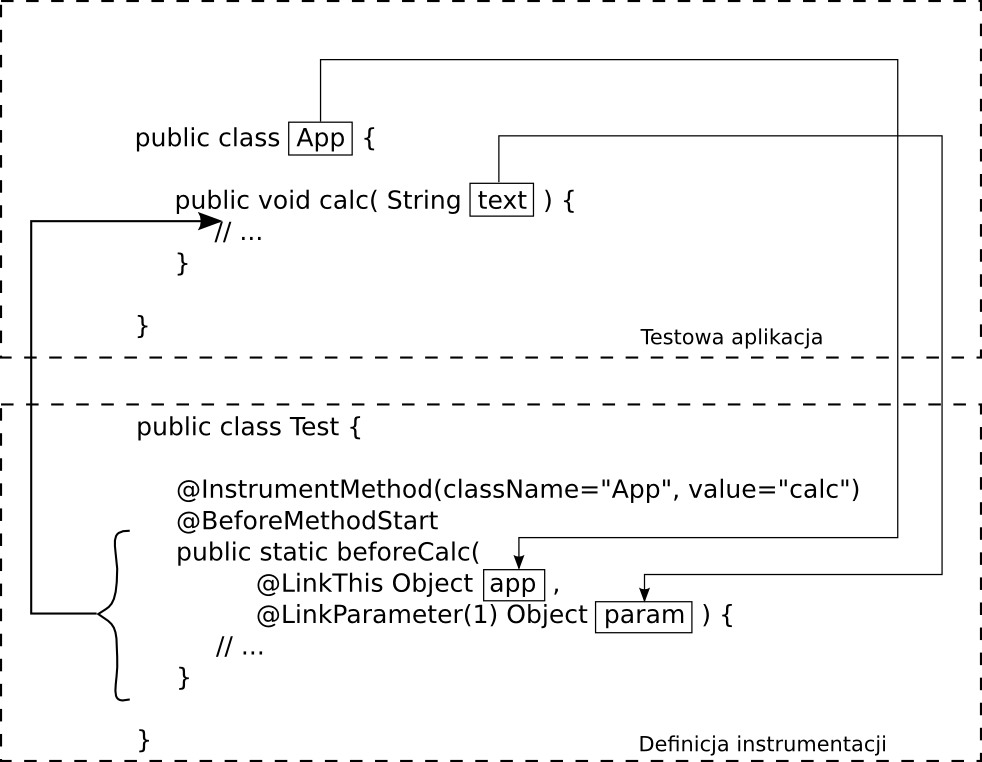
\includegraphics[bb=0 0 376 292]{implementation/instr.png}
 % instr.png: 982x762 pixel, 188dpi, 13.27x10.29 cm, bb=0 0 376 292
 \caption{Przyk�ad u�ycia biblioteki instrumentuj�cej kod}
 \label{fig:impl:instr}
\end{figure}

Adnotacje dla biblioteki instrumentuj�cej kod umieszczone s� w cz�ci sensora wydajno�ci charakterystycznej dla danego kontenera. Pozwalaj� sensorowi zbiera� dane w trakcie dzia�ania us�ug (np. rozpocz�to wykonywanie operacji webservice, zako�czono wykonywanie operacji webservice). Dane te tworz� komunikat w zestandaryzowanej postaci, kt�ry jest przekazywany do cz�ci sensora niezale�nej od konkretnego kontenera.

\subsection{Format komunikatu z danymi o wydajno�ci}

Format komunikatu z danymi o wydajno�ci zosta� przedstawiony na rysunku~\ref{fig:impl:message}.

\begin{figure}[htb!]
 \centering
 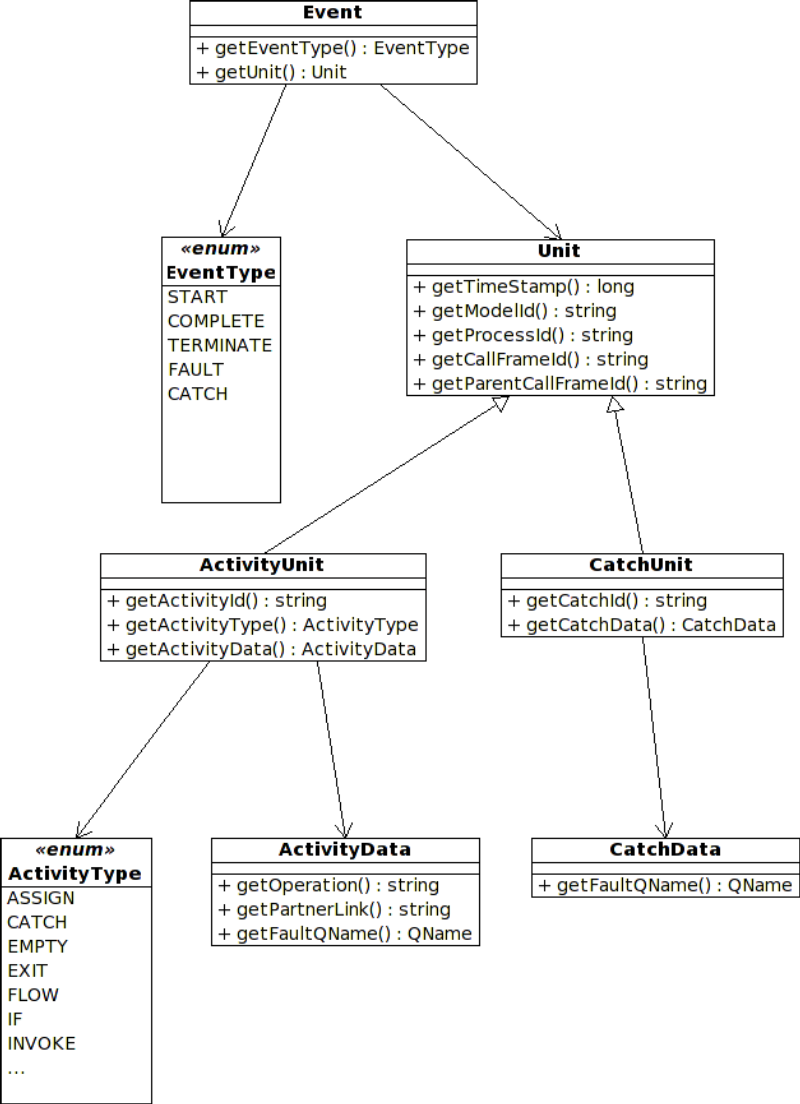
\includegraphics[bb=0 0 384 530]{implementation/message.png}
 % message.png: 800x1104 pixel, 150dpi, 13.55x18.69 cm, bb=0 0 384 530
 \caption{Posta� komunikatu z danymi o wydajno�ci w postaci diagramu klas UML}
 \label{fig:impl:message}
\end{figure}

G��wna klasa komunikatu (Event) mo�e przenosi� jeden z dw�ch rodzaj�w zdarze�:
\begin{itemize}
 \item{ActivityUnit} - je�li zdarzenie dotyczy aktywno�ci procesu BPEL (np. invoke, assign). Mo�liwe zdarzenia okre�lone s� w�wczas przez warto�� EventType:
  \begin{itemize}
   \item{START} - rozpocz�to wykonywanie aktywno�ci.
   \item{COMPLETE} - poprawnie wykonano aktywno��.
   \item{FAULT} - wykonywanie aktywno�ci zako�czy�o si� wyj�tkiem.
   \item{TERMINATE} - wykonywanie aktywno�ci zosta�o przerwane (np. z powodu wyj�tku w podwykonywanej aktywno�ci).
  \end{itemize}
 \item{CatchUnit} - je�li zdarzenie dotyczy obs�ugi sytuacji wyj�tkowej.
\end{itemize}


W miar� otrzymywania kolejnych danych od sensora wydajno�ci w konsoli budowany jest model zachodz�cego procesu. Konsola nie ma dost�pu do oryginalnych modeli proces�w przechowywanych w kontenerach aplikacji, dlatego do zbudowania modelu procesu musz� jej wystarczy� dane otrzymywane z sensora wydajno�ci. Powoduje to konieczno�� sformu�owania dodatkowych za�o�e� dotycz�cych identyfikator�w otrzymywanych w wiadomo�ciach z rysunku \ref{fig:impl:message}:
\begin{itemize}
 \item identyfikator modelu procesu (unikalny globalnie)
 \item identyfikator procesu - wskazuje konkretne wywo�anie procesu wed�ug danego modelu (unikalny globalnie)
 \item identyfikator aktywno�ci - wyra�enie XPATH\cite{impl:xpath} wskazuj�ce na aktywno�� z modelu procesu (unikalny w obr�bie modelu)
 \item identyfikator w�tku (unikalny w obr�bie procesu)
 \item identyfikator w�tku-rodzica (unikalny w obr�bie procesu)
\end{itemize}

Komunikat w formacie zgodnym z rysunkiem \ref{fig:impl:instr} jest przekazywany do cz�ci sensora niezale�nej od u�ywanego kontenera. Odpowiada ona za przekazywanie komunikat�w do konsoli prezentuj�cej wyniki.

\subsection{Przekazywanie wiadomo�ci od sensora do konsoli}

Komunikaty wysy�ane s� z sensora do serwera JMS, sk�d mog� by� pobierane przez konsol� prezentuj�c� wyniki. Proces wysy�ania komunikat�w odbywa si� niezale�nie od ich generowania, utworzone przez sensor komunikaty s� umieszczane w kolejce, z kt�rej okresowo s� pobierane i przekazywane do serwera JMS przez osobny w�tek. Pozwala to zminimalizowa� wp�yw sensora na dzia�anie badanych us�ug - jedyny dodatkowy narzut zwi�zany z umieszczaniem komunikat�w w kolejce jest bardzo ma�y. U�ycie serwera JMS zapewnia prosty i pewny spos�b na dostarczenie danych do konsoli. W praktyce przekazywanie wiadomo�ci do serwer�w JMS wymaga dodania dodatkowej grupy bibliotek (np. bibliotek Service Provider dla JNDI \cite{impl:jndi_spi}). Biblioteki te musz� by� dodane do kontenera, poniewa� kontener zosta� zinstrumentowany przez sensor wydajno�ci wysy�aj�cy komunikaty JMS. Powoduje to mo�liwo�� powstawania konflikt�w wersji z istniej�cymi ju� bibliotekami wchodz�cymi w sk�ad kontener�w (wsparcie dla serwer�w JMS jest powszechne w kontenerach). Problem ten mo�na rozwi�za� stosuj�c koncepcj� podobn� do tzw. sandbox\cite{impl:sandbox}. Biblioteki serwera JMS nie s� bezpo�rednio do��czane do kontenera, tylko do izolowanego �rodowiska (sandbox) dzia�aj�cego w obr�bie kontenera. W �rodowisku tym dzia�a kod odpowiedzialny za wysy�anie komunikat�w do serwera JMS. Poza izolowanym �rodowiskiem nie s� widoczne biblioteki serwera JMS dlatego nie powoduj� one interakcji z kontenerem. Przedstawion� koncepcj� sposobu przekazywania wiadomo�ci od sensora do konsoli ilustruje rysunek \ref{fig:impl:flow}.

\begin{figure}[htb!]
 \centering
 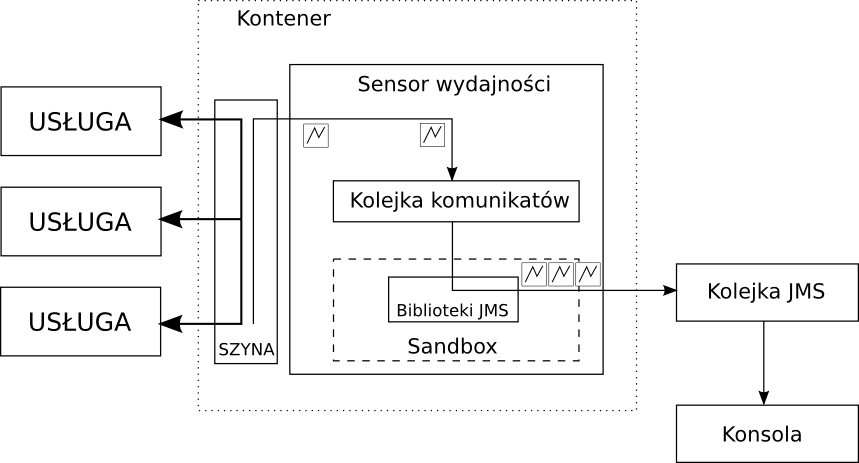
\includegraphics[bb=0 0 329 177]{implementation/flow.png}
 % flow.png: 859x463 pixel, 188dpi, 11.60x6.26 cm, bb=0 0 329 177
 \caption{Przep�yw komunikat�w z danymi o wydajno�ci}
 \label{fig:impl:flow}
\end{figure}


\subsection{Wizualizacja zebranych danych w konsoli}

Cz�� prezentacyjna projektu zosta�a wykonana z u�yciem komponent�w z modu�u BPEL Designer pakietu NetBeans 6.0. Komponenty te nie s� dost�pne jako oddzielna biblioteka, lecz stanowi� integraln� cz�� tego �rodowiska. Chc�c je wykorzysta� w innej aplikacji konieczne by�o zamkni�cie ich w kontenerze symuluj�cym oryginalne �rodowisko (sytuacja przedstawiona na rys. \ref{fig:netbeans_emulation}). 

\begin{figure}[htb!]
 \centering
 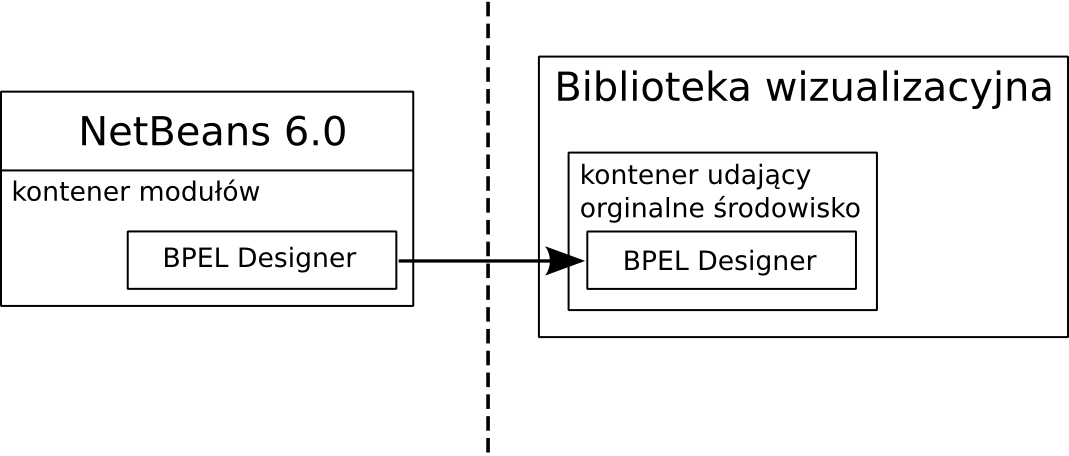
\includegraphics[bb=0 0 257 109]{implementation/netbeans_emulation.png}
 % netbeans_emulation.png: 332x141 pixel, 93dpi, 9.07x3.85 cm, bb=0 0 257 109
 %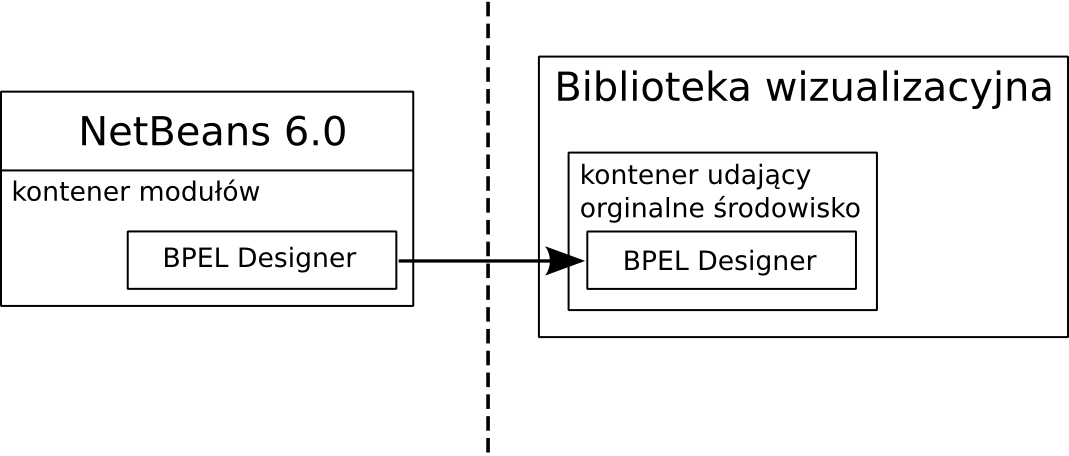
\includegraphics[bb=0 0 239 110]{implementation/netbeans_emulation.png}
 %% netbeans_emulation.png: 311x143 pixel, 94dpi, 8.41x3.87 cm, bb=0 0 239 110
 \caption{Emulacja �rodowiska NetBeans 6.0 w bibliotece wizualizacyjnej}
 \label{fig:netbeans_emulation}
\end{figure}

Aby emulowa� �rodowisko NetBeans w satysfakcjonuj�cym stopniu konieczne by�o podj�cie nast�puj�cych krok�w:
\begin{itemize}
 \item implementacja w�asnej klasy realizuj�cej rejestr obiekt�w �rodowiska (realizacja interfejsu org.openide.util.Lookup) i zape�nienie go wymaganymi warto�ciami
 \item stworzenie w�asnej klasy realizuj�cej interfejs org.openide.loaders.DataObject reprezentuj�cej obiekt z danymi w NetBeans
 \item stworzenie szkieletu obiektu reprezentuj�cego pusty dokument procesu BPEL
 \item zarz�dzanie skomplikowanym cyklem �ycia obiektu reprezentuj�cego model procesu BPEL
\end{itemize}

Efektem tych dzia�a� jest kompletna biblioteka pozwalaj�ca na przedstawianie procesu BPEL w efektownej formie graficznej. Komponent wizualizacyjny zosta� zrealizowany jako obiekt rozszerzaj�cy znany ze �rodowiska Swing JPanel\footnote{org. javax.swing.JPanel}, co pozwala na jego proste u�ycie. Przyk�adowy kod realizuj�cy wy�wietlenie prostego procesu BPEL wygl�da nast�puj�co:

\begin{lstlisting}[frame=tb]
 // inicjalizacja g��wnego obiektu widoku
 BPELVisualisationView view =
   BPELVisualisationView.createViewWithEmptyModel("anyDesign", 
                                                  "anyNS");
 // pobranie referencji do modelu procesu BPEL
 BpelModel model = view.getBPELModel();
 // pobranie referencji do obiektu buduj�cego elementy procesu
 BPELElementsBuilder builder = model.getBuilder();

 // zbudowanie sekwencji 
 Sequence sequence = builder.createSequence();
 // ustawienie sekwencji jako g��wnej aktywno�ci procesu
 model.getProcess().setActivity(sequence);

 // stworzenie aktywno�ci przypisania zmiennej
 Assign assign = builder.createAssign();
 // dodanie aktywno�ci do sekwencji
 sequence.addActivity(assign);

 // poinformowanie obiektu widoku o zmianach
 view.commitChanges();
\end{lstlisting}

Przyk�adowy wynik dzia�ania, dla bardziej skomplikowanego przypadku jest przedstawiony na rysunku \ref{fig:designer_complicated}

\begin{figure}[htb!]
 \centering
 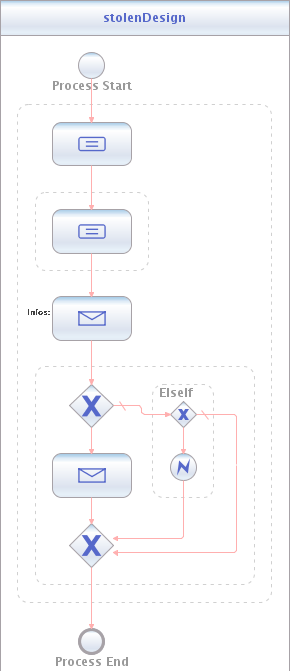
\includegraphics[bb=0 0 139 322]{implementation/designer_complicated.png}
 % designer_complicated.png: 290x671 pixel, 150dpi, 4.91x11.36 cm, bb=0 0 139 322
 \caption{Przyk�adowy wynik dzia�ania cz�ci wizualizacyjnej}
 \label{fig:designer_complicated}
\end{figure}

\newpage


\paragraph{Rozszerzenia} Z uwagi na zastosowanie biblioteki, zosta�a ona rozszerzona o dwie dodatkowe funkcjonalno�ci
\begin{itemize}
 \item mo�liwo�� etykietowania aktywno�ci procesu BPEL - celem dodawania informacji odno�nie dokonanych pomiar�w
 \item mo�liwo�� zmiany koloru po��cze� mi�dzy aktywno�ciami - celem ukazania cz�sto�ci wykorzystania poszczeg�lnych �cie�ek w procesie (np. na rysunku \ref{fig:impl:designer_paths} po��czenie wychodz�ce od INVOKE nie by�o u�ywane, wi�c ma inny kolor ni� reszta po��cze�)
\end{itemize}
Co istotne, zmiany te zosta�y dokonane bez ingerencji w oryginalny kod BPEL Designer.

\begin{figure}[htb!]
 \centering
 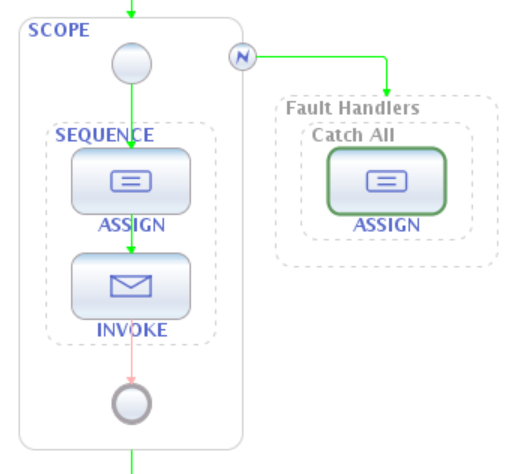
\includegraphics[bb=0 0 246 228]{implementation/designer_paths.png}
 % designer_paths.png: 513x474 pixel, 150dpi, 8.69x8.03 cm, bb=0 0 246 228
 \caption{Fragment wizualizacji procesu BPEL wykorzystuj�cy zmian� koloru danego po��czenia w celu pokazania cz�sto�ci jego u�ycia}
 \label{fig:impl:designer_paths}
\end{figure}

Biblioteka zosta�a przygotowana jako niezale�na cz�� i mo�e z powodzeniem by� wykorzystywana w innych rozwi�zaniach.

\newpage

\section{Podsumowanie}

Po rozwi�zaniu wszystkich (m.in. przedstawionych w niniejszym rozdziale) problem�w uda�o si� stworzy� aplikacj� do badania wydajno�ci us�ug zrealizowanych w architekturze SOA zgodnie z za�o�eniami przedstawionymi w rozdziale 3 i 4. Aplikacja otrzyma�a robocz� nazw� BPEL Profiler, kt�rej autorzy u�ywaj� w dalszej cz�ci pracy.

Przyk�adowe regu�y instrumentacji zosta�y opracowane dla kontener�w us�ug obs�uguj�cych OpenESB. Praktyczne sprawdzenie zrealizowanej aplikacji w �rodowisku testowym zosta�o przedstawione w kolejnym rozdziale.

\chapter{Testy}

W niniejszym rozdziale opisana zosta�a procedura testowania z u�yciem narz�dzia BPEL Profiler. 
Przedstawiono spos�b konfiguracji sprz�tu i oprogramowania �rodowiska testowego, oraz opisano aplikacje b�d�ce materia�em do test�w. Rozdzia� zawiera r�wnie� wyniki dzia�ania stworzonego narz�dzia.

\section{Testowane oprogramowanie}

Testy zosta�y przeprowadzone na przyk�adowych aplikacjach BPEL dostarczanych przez firm� Sun \texttrademark - BPEL Blueprints. S� to proste, wzorcowe rozwi�zania problem�w integracyjnych z u�yciem j�zyka BPEL\cite{tests:blueprints}. Poni�ej przedstawiono kr�tki opis  ka�dego z nich.

\paragraph{Aplikacja realizuj�ca synchroniczne wywo�anie us�ugi}
Jest to prosty proces realizuj�cy integracj� sklepu z magazynem. Graficzna prezentacja procesu BPEL jest przedstawiona na rysunku 5.1.
%\ref{tests:blueprint1}.

\begin{figure}
 \centering
 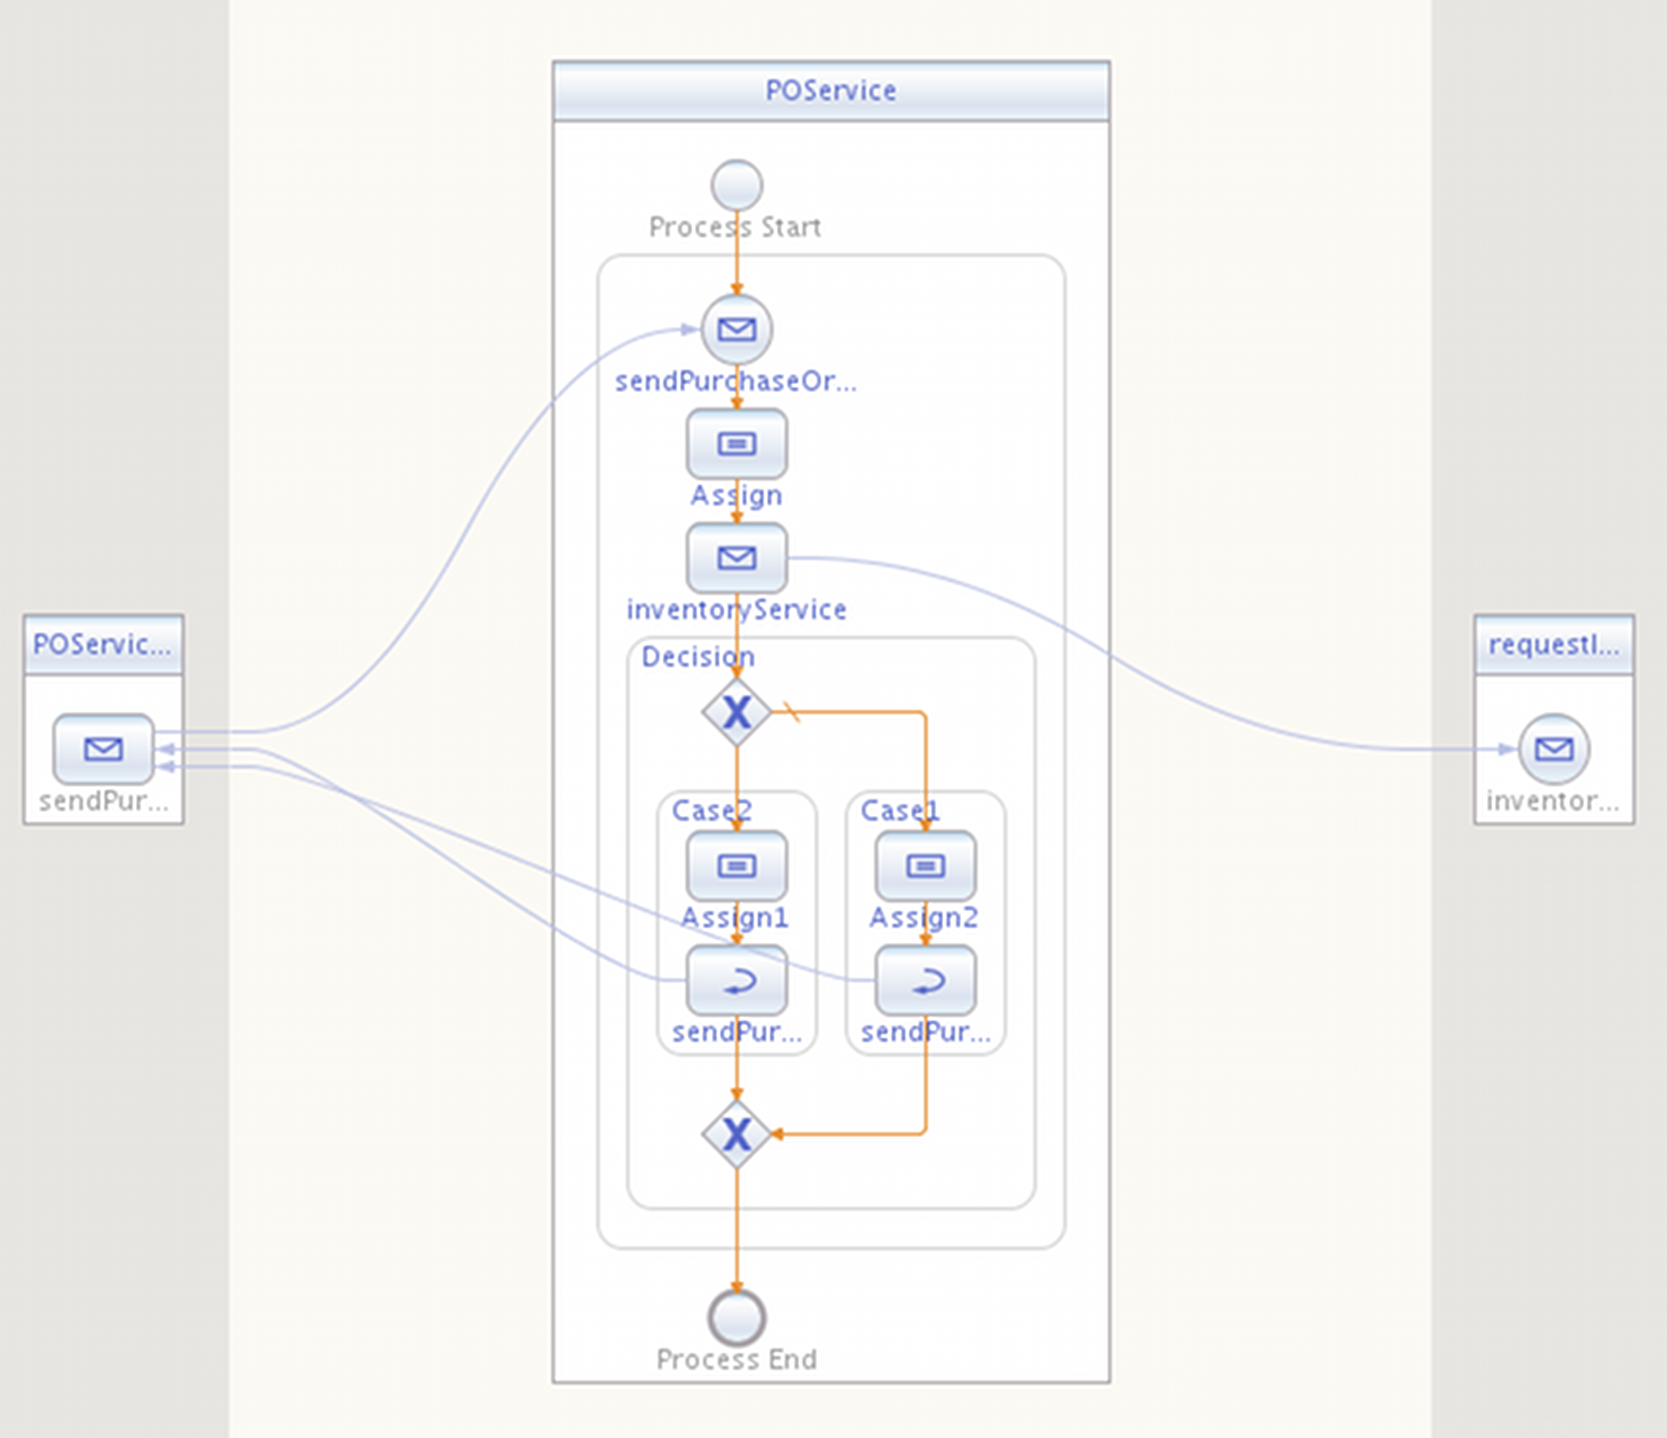
\includegraphics[bb=0 0 400 345]{tests/blueprint1_process.png}
 % blueprint1_process.png: 1667x1438 pixel, 300dpi, 14.11x12.18 cm, bb=0 0 400 345
 \label{tests:blueprint1}
 \caption{Aplikacja realizuj�ca synchroniczne wywo�anie us�ugi}
\end{figure}

Na podstawie przychodz�cych do interfejsu sklepu (POServicePlink) ��da� nast�puje synchroniczne odpytanie us�ugi magazynu (requestInventoryPlink) o dost�pno�� produktu. W zale�no�ci od odpowiedzi magazynu, us�uga sklepu potwierdza lub odmawia z�o�enia zam�wienia.

\paragraph{Aplikacja realizuj�ca asynchroniczne wywo�anie us�ugi}

Proces realizuj�cy tak� sam� funkcjonalno�� jak poprzedni. R�ni� si� one jedynie sposobem komunikacji z magazynem - w tym przypadku, wywo�anie us�ugi magazynu jest jednokierunkowe. Nast�pnie proces oczekuje na jedno ze zdarze� z bloku EventBasedDecision - nadej�cie odpowiedzi lub up�yni�cie limitu czasowego. Odpowied� wysy�ana do klienta jest zale�na od tej odpowiedzi. Prezentacja graficzna procesu znajduje si� na rysunku 5.2.
%\ref{tests:blueprint2}

\begin{figure}
 \centering
 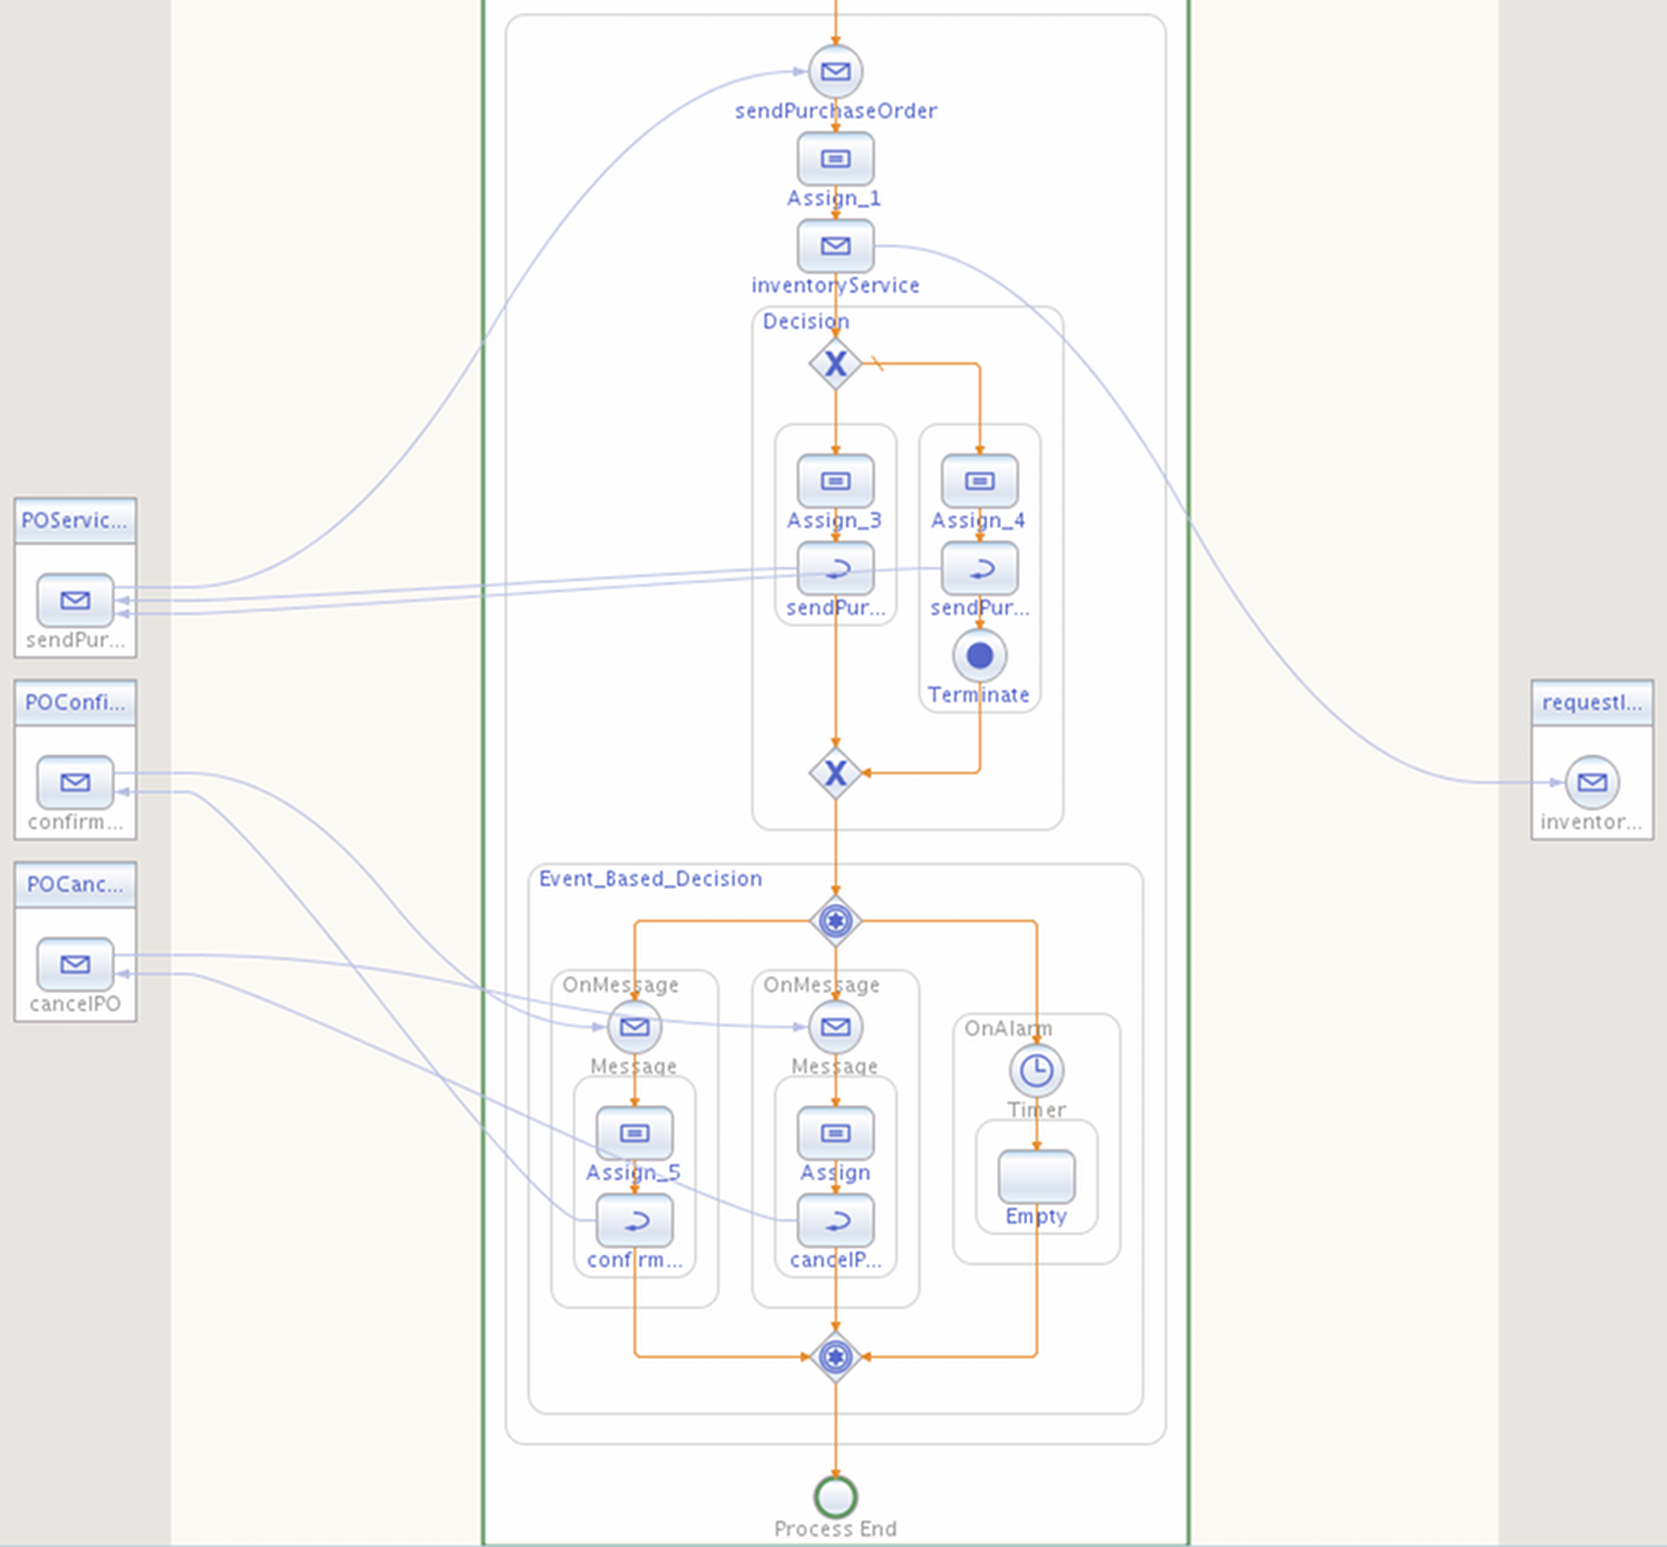
\includegraphics[bb=0 0 400 371]{tests/blueprint2_process.png}
 % blueprint2_process.png: 1667x1547 pixel, 300dpi, 14.11x13.10 cm, bb=0 0 400 371
 \label{tests:blueprint2}
 \caption{Aplikacja realizuj�ca asynchroniczne wywo�anie us�ugi}
\end{figure}

\paragraph{Aplikacja realizuj�ca synchroniczne wywo�anie us�ugi z obs�ug� wyj�tk�w}
Rozszerzenie pierwszego procesu o mechanizm obs�ugi wyj�tk�w - proces pocz�tkowo sprawdza poprawno�� przychodz�cego zam�wienia, w wypadku b��du rzuca wyj�tek. Drugim obs�ugiwanym wyj�tkiem jest sygnalizowany przez magazyn brak zamawianego produktu. Graficzna prezentacja procesu znajduje si� na rysunku 5.3. %\ref{tests:blueprint3}.

\begin{figure}
 \centering
 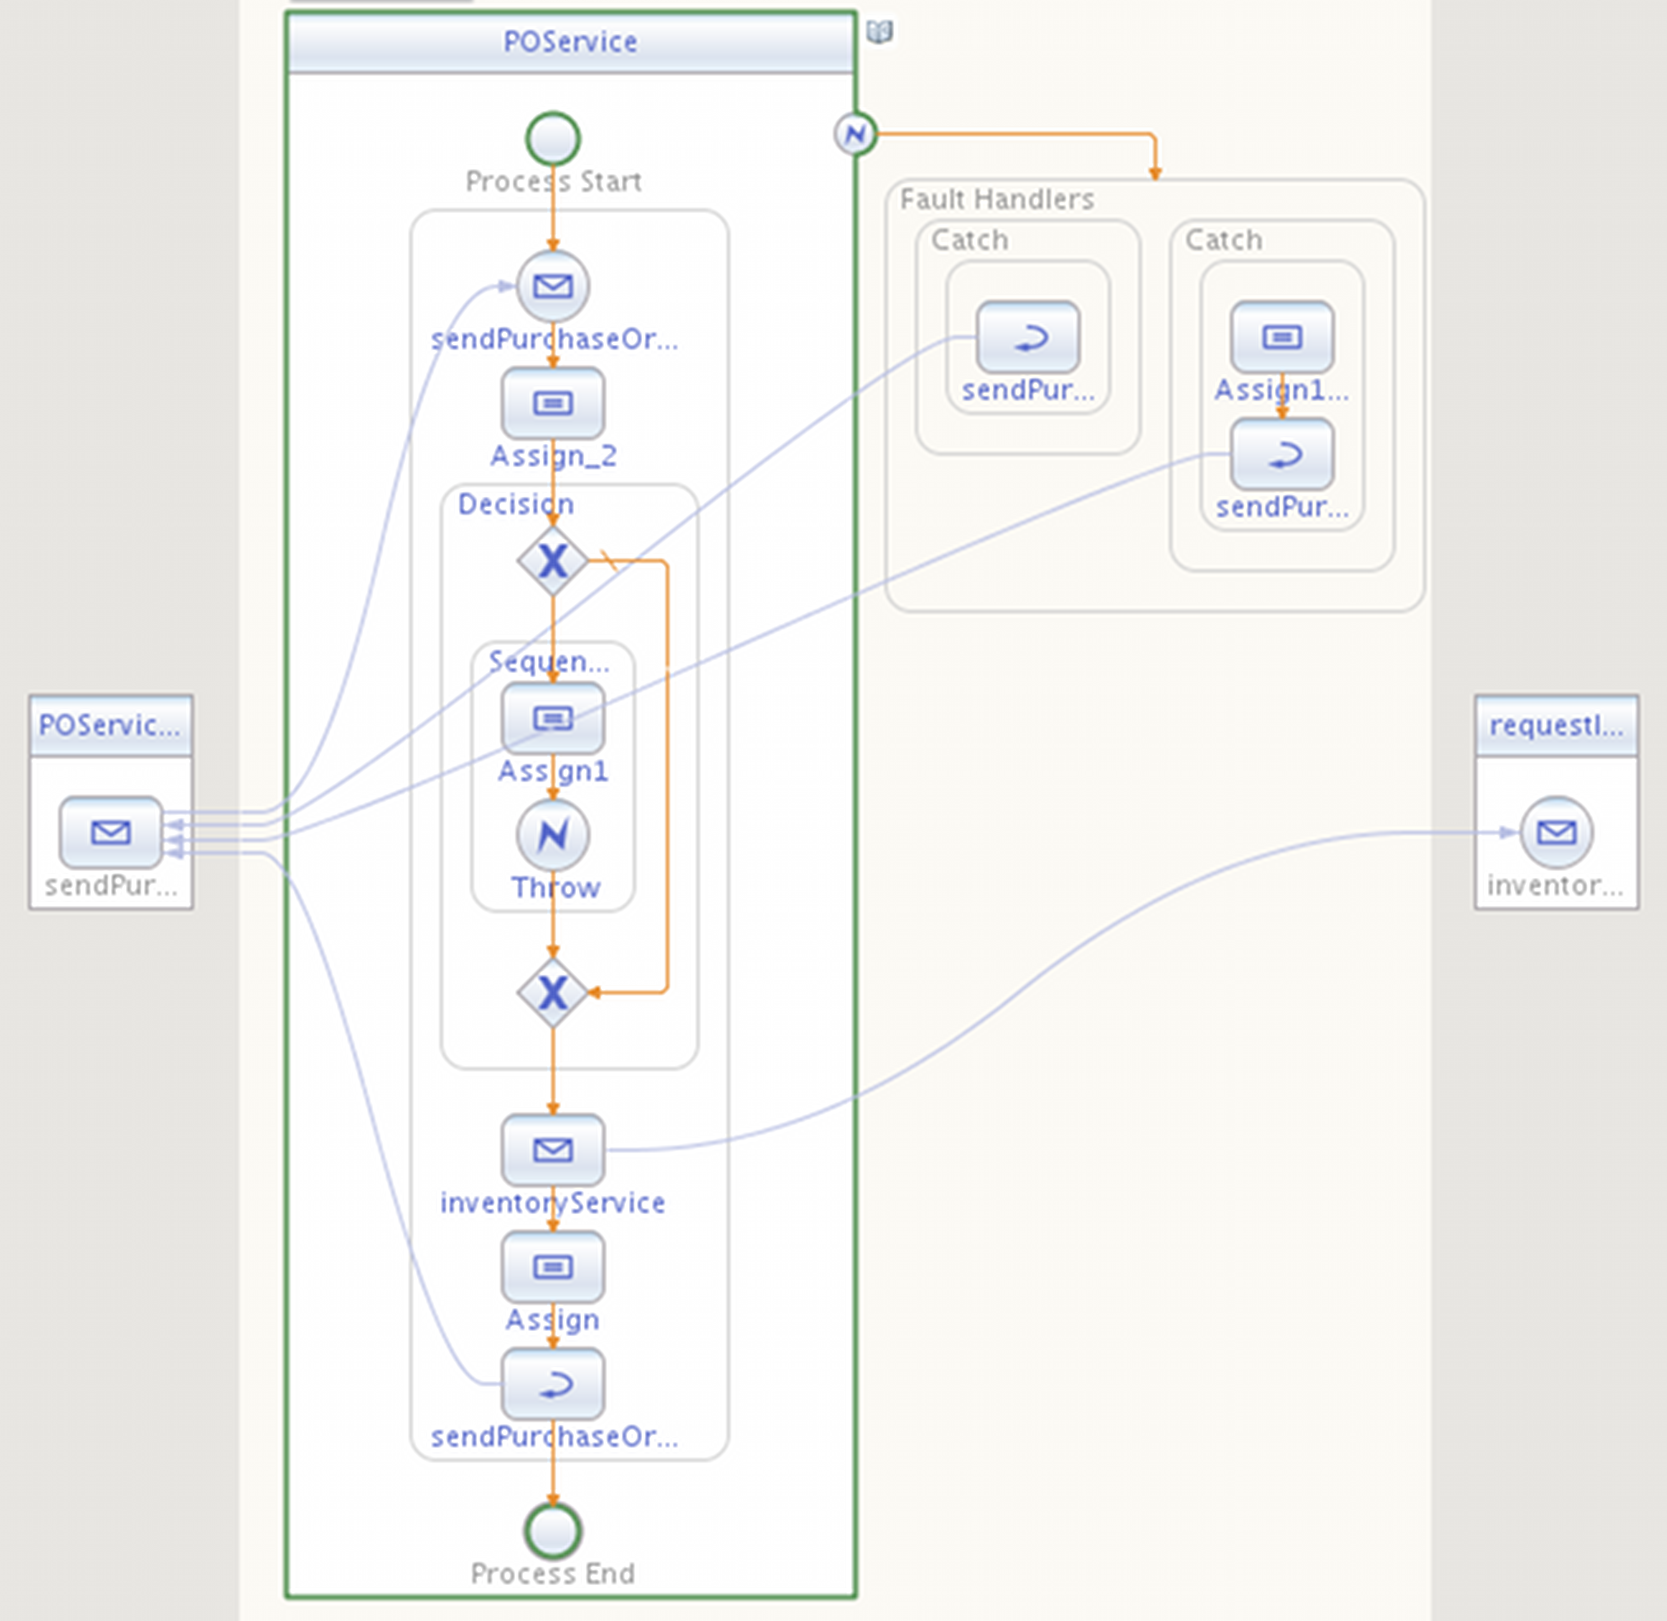
\includegraphics[bb=0 0 400 389]{tests/blueprint3_process.png}
 % blueprint3_process.png: 1667x1621 pixel, 300dpi, 14.11x13.72 cm, bb=0 0 400 389
  \label{tests:blueprint3}
 \caption{Aplikacja realizuj�ca obs�ug� wyj�tk�w rzucanych z procesu oraz wykorzystywanych us�ug}
\end{figure}

\paragraph{Aplikacja koreluj�ca kilka wywo�a�}

Proces b�d�cy rozszerzeniem pierwszego wariantu, o mo�liwo�� potwierdzenia lub anulowania zam�wienia. Po z�o�eniu zam�wienia, aplikacja czeka na dalsze instrukcje, lub up�yni�cie limitu czasowego, po czym podejmuje stosowne do zdarzenia akcje. Korelacja jest realizowana poprzez zawarcie w przesy�anych wiadomo�ciach parametr�w pozwalaj�cych na zidentyfikowanie instancji procesu dla kt�rego przeznaczona jest dana wiadomo��. Graficzna prezentacja procesu znajduje si� na rysunku 5.4.
%\ref{tests:blueprint4}.

\begin{figure}
 \centering
 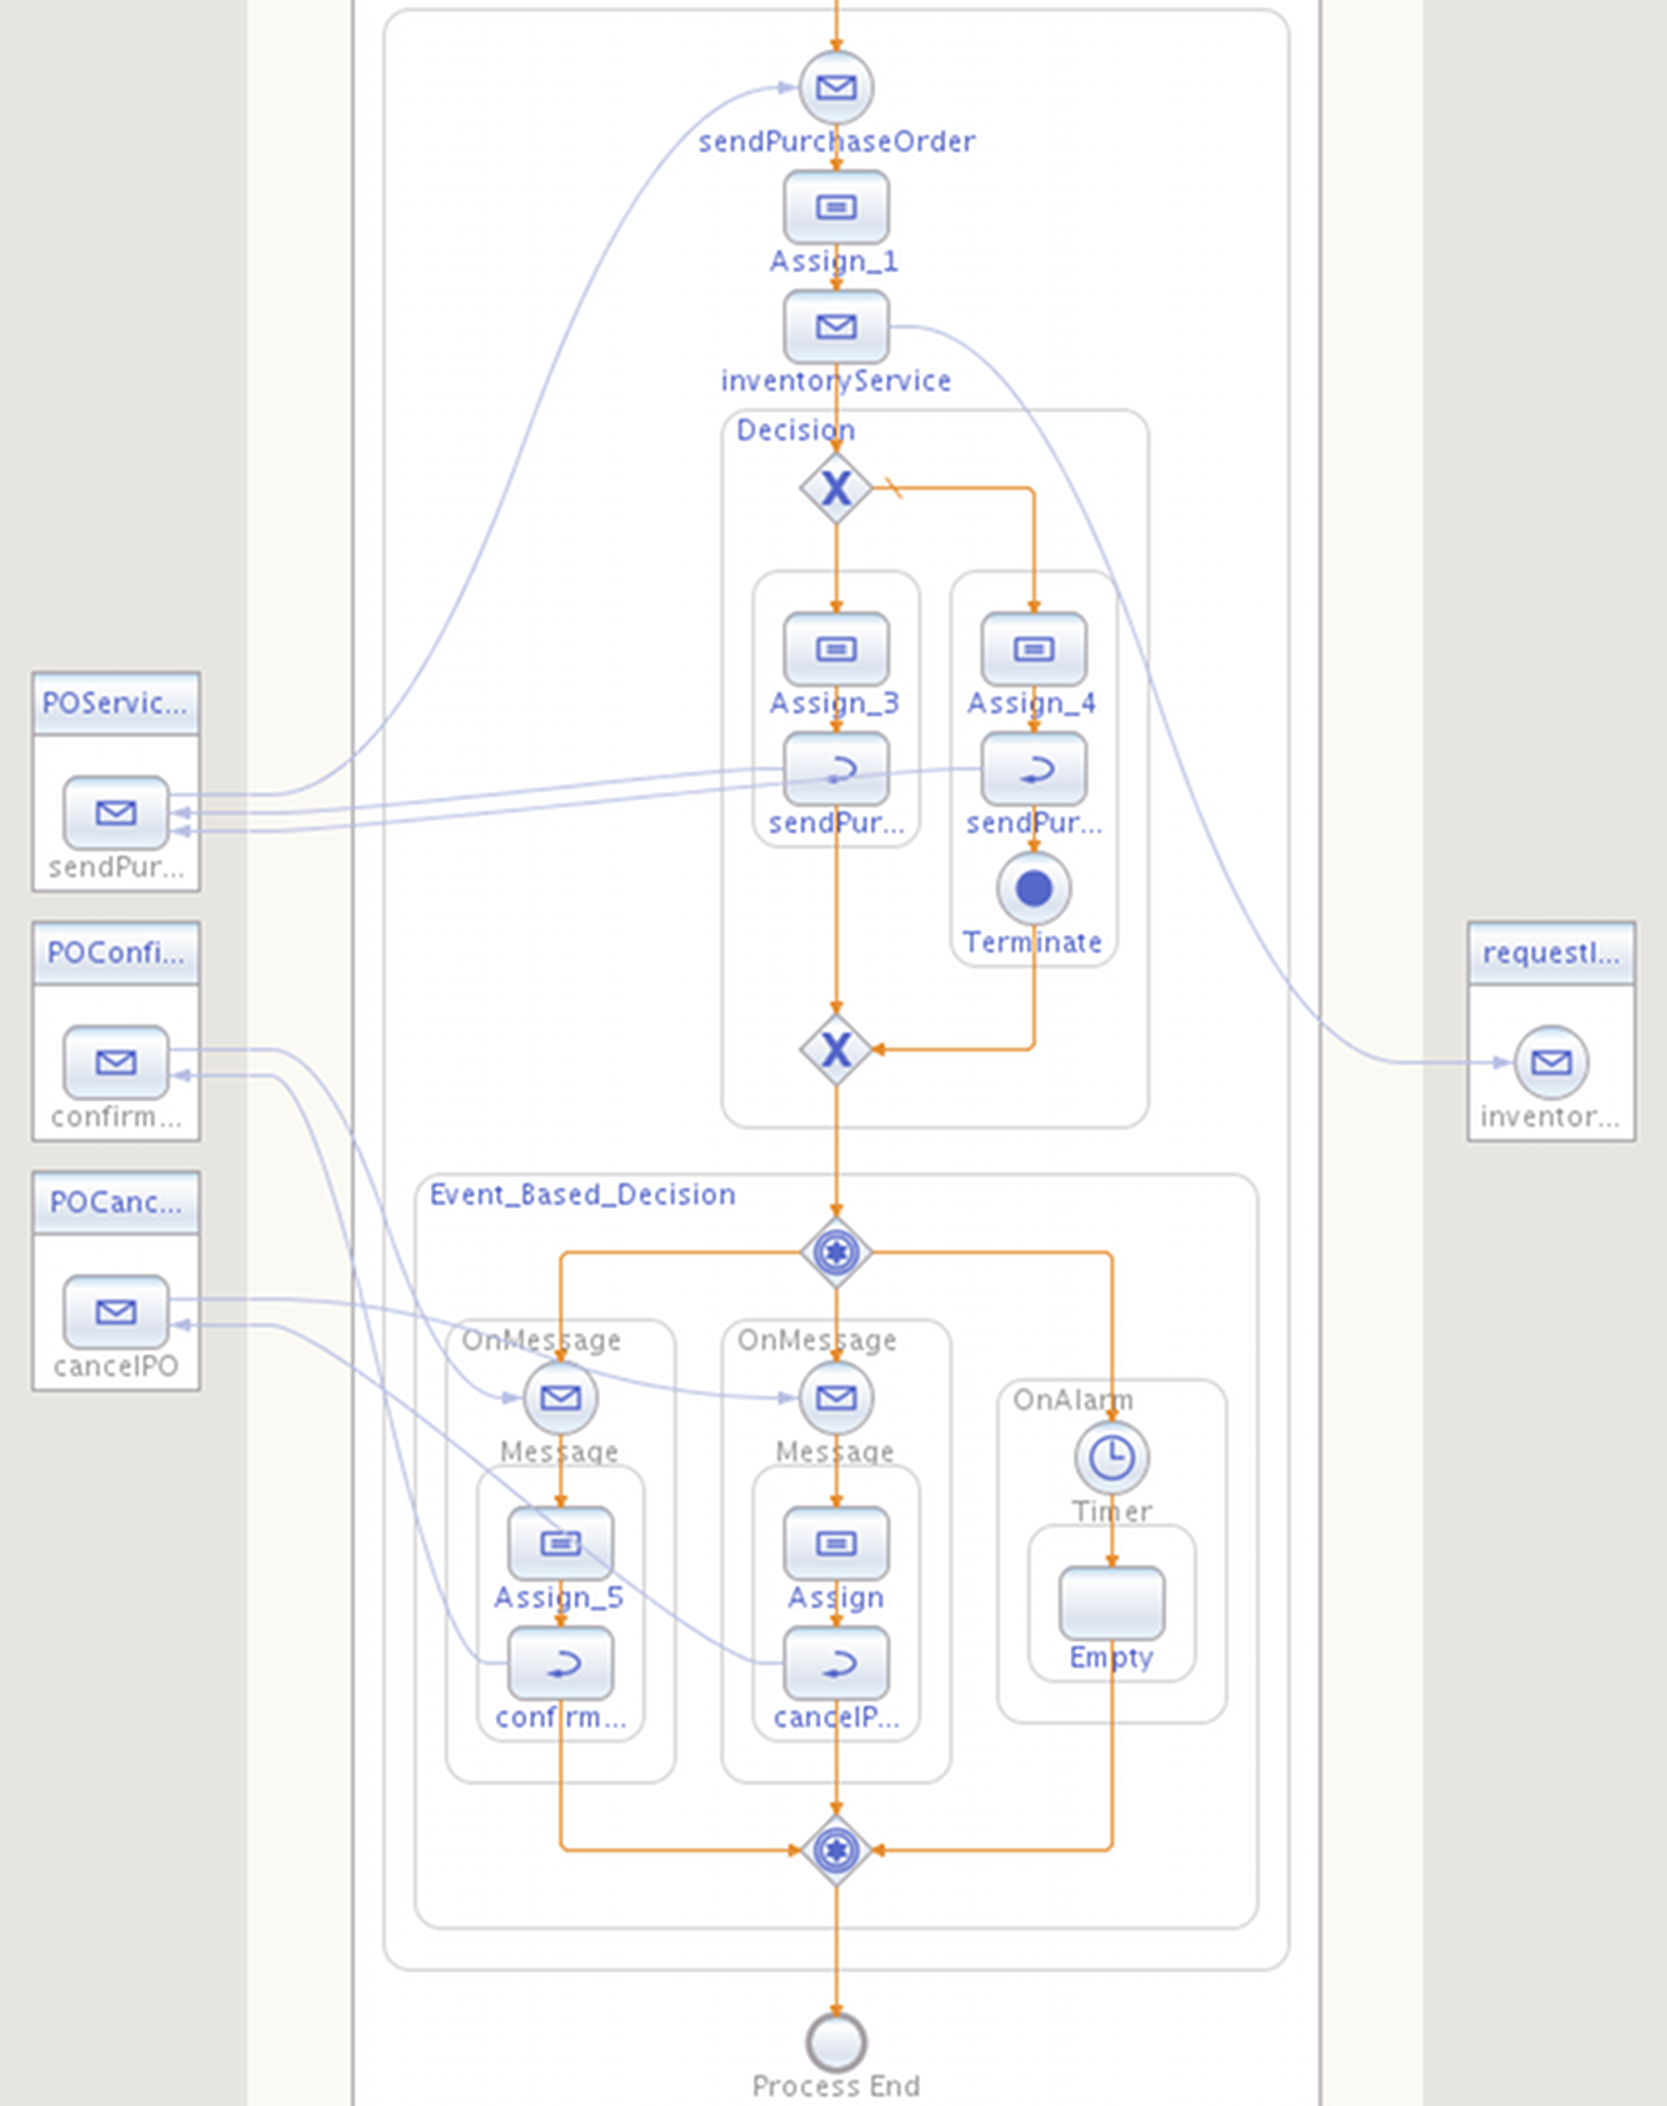
\includegraphics[bb=0 0 400 505]{tests/blueprint4_process.png}
 % blueprint4_process.png: 1667x2106 pixel, 300dpi, 14.11x17.83 cm, bb=0 0 400 505
 \label{tests:blueprint4}
 \caption{Aplikacja koreluj�ca kilka wywo�a� dotycz�cych tej samej instancji procesu}
\end{figure}

\paragraph{Aplikacja realizuj�ca r�wnoleg�e asynchroniczne wywo�anie kilku us�ug}

Proces realizuj�cy wycinek funkcjonalno�ci biura turystycznego, pozwalaj�cego na jednoczesn� rezerwacj� biletu lotniczego, hotelu i samochodu. Realizuje on r�wnoleg�e wykonanie trzech asynchronicznych wywo�a� us�ug rezerwacji, kt�rych wynik jest zwracany do klienta. Reprezentacja graficzna procesu znajduje si� na rysunku 5.5. %\ref{tests:blueprint5}. 

\begin{figure}
 \centering
 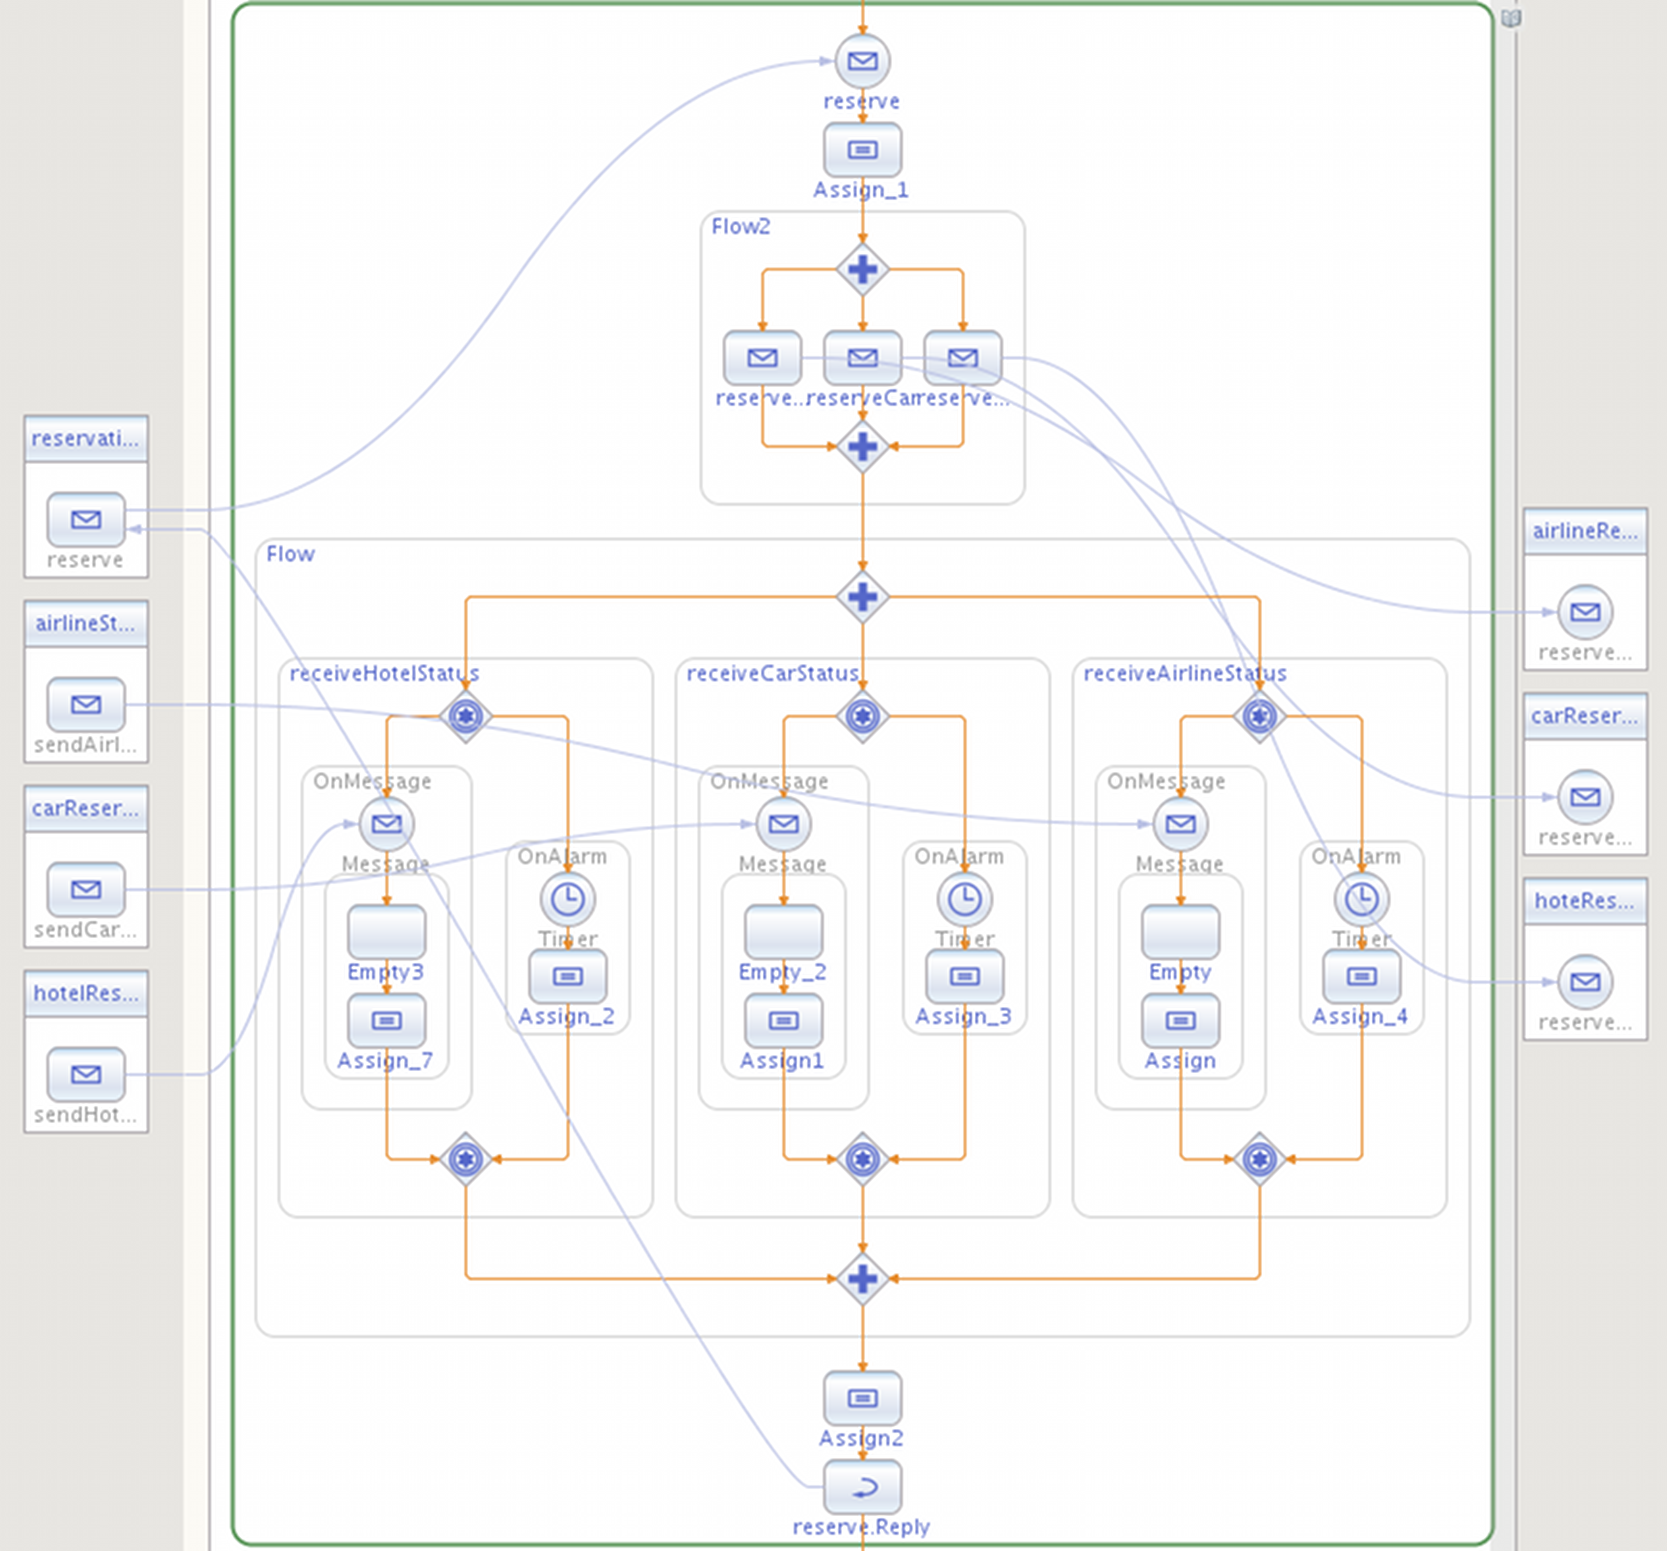
\includegraphics[bb=0 0 400 372]{tests/blueprint5_process.png}
 % blueprint5_process.png: 1667x1551 pixel, 300dpi, 14.11x13.13 cm, bb=0 0 400 372
 \label{tests:blueprint5}
 \caption{Aplikacja realizuj�ca r�wnoleg�e asynchroniczne wywo�anie us�ug}
\end{figure}

\newpage

\section{Opis procedury testowania}

Procedur� testowania realizowano wed�ug nast�puj�cego schematu:

\begin{itemize}
 \item Instalacja testowanej aplikacji w �rodowisku OpenESB 
 \item Wyzwolenie procesu testowanej us�ugi 
 \item Obserwacja wynik�w na konsoli wizualizacyjnej
\end{itemize}

Wyzwalanie procesu powtarzano dla r�nych danych celem ukazania mo�liwo�ci budowania procesu w locie oraz agregowania wynik�w ko�cowych.

\paragraph{Analiza intruzywno�ci pomiaru} 
Zaburzenie zbieranych wynik�w mo�e zosta� przeanalizowane w dw�ch aspektach:
\begin{itemize}
 \item Modyfikacja infrastruktury spowodowana wysy�aniem dodatkowych komunikat�w z danymi o wydajno�ci. Serwer JMS oraz konsola wizualizacyjna znajduj� si� zwykle na osobnej maszynie, celem zniwelowania ich wp�ywu na badane us�ugi. Stosowane ��cza pomi�dzy maszynami maj� zwykle bardzo du�� przepustowo�� (np. \nolinebreak{1 Gbps} w izolowanym �rodowisku testowym) co przy ma�ym rozmiarze komunikat�w o wydajno�ci powoduje, �e wp�yw dodatkowych komunikat�w z danymi o wydajno�ci na badane us�ugi jest pomijalny.
 \item Zbieranie dodatkowych danych o wydajno�ci zaburza natur� badanych us�ug. Wybrany spos�b instrumentacji i zbierania danych nie powoduje du�ych narzut�w czasowych. Proces wysy�ania danych do kolejki JMS odbywa si� asynchronicznie, co r�wnie� nie zaburza wynik�w w znacznym stopniu.
\end{itemize}
Zastosowany spos�b zbierania danych nie ma znacz�cego wp�ywu na badane us�ugi. Dok�adne badania s� trudne do przeprowadzenia z uwagi na brak por�wnywalnego narz�dzia do badania wydajno�ci us�ug opartych o paradygmat SOA.

\paragraph{Weryfikacja wynik�w}
Weryfikacja zebranych wynik�w mo�e zosta� dokonana w dw�ch aspektach:
\begin{itemize}
 \item Zgodno�� pomi�dzy oryginalnym modelem biznesowym a wygenerowanym modelem w konsoli wizualizacyjnej. Zgodno�� stwierdzana jest na podstawie wizualnego por�wnaniu obu modeli.
 \item Poprawno�� zebranych danych (statystyk czasowych). Weryfikacja zebranych danych liczbowych jest trudna do przeprowadzenia, z powodu braku por�wnywalnych narz�dzi do badania wydajno�ci us�ug opartych o paradygmat SOA. Jedynym wyznacznikiem poprawno�ci zebranych danych mo�e by� ich zgodno�� z warto�ciami szacunkowymi dla danego modelu (np. przy zastosowaniu konstrukcji WAIT z parametrem 2 sekundy, czas wykonania takiej aktywno�ci powinien wynosi� co najmniej 2 sekundy).
\end{itemize}
Weryfikacja otrzymanych wynik�w jest bardzo trudna do przeprowadzenia. Mo�na jedynie wizualnie oceni� otrzymane warto�ci.

%Instrumentacja kodu silnika BPEL �rodowiska wykonawczego nie pozostaje bez wp�ywu na czas wykonania procesu. Nale�y jednak zwr�ci� uwag�, i� z uwagi na spos�b instrumentacji wzrost czasu wykonania nie wp�ywa znacz�co na wyniki otrzymywane dla ka�dej aktywno�ci. Stopie� wp�ywu pomiar�w na czas wykonania procesu jest g��wnie determinowany przez szybko�� dzia�ania zastosowanego rozwi�zania MOM (w przypadku przyk�adowej procedury - OpenJMS).

\section{Konfiguracja infrastruktury}

Konfiguracj� infrastruktury przedstawia rysunek \ref{fig:tests:deployment}. Na Serwerze 1 zainstalowano zinstrumentowane �rodowisko wykonawcze, i umieszczano na nim kolejne testowana aplikacje. Serwer JMS i konsola wizualizacyjna (na Serwrze 2) zosta�y odizolowane od �rodowiska wykonawczego, celem zminimalizowania ich wp�ywu na wyniki test�w.

\begin{figure}[htb!]
 \centering
 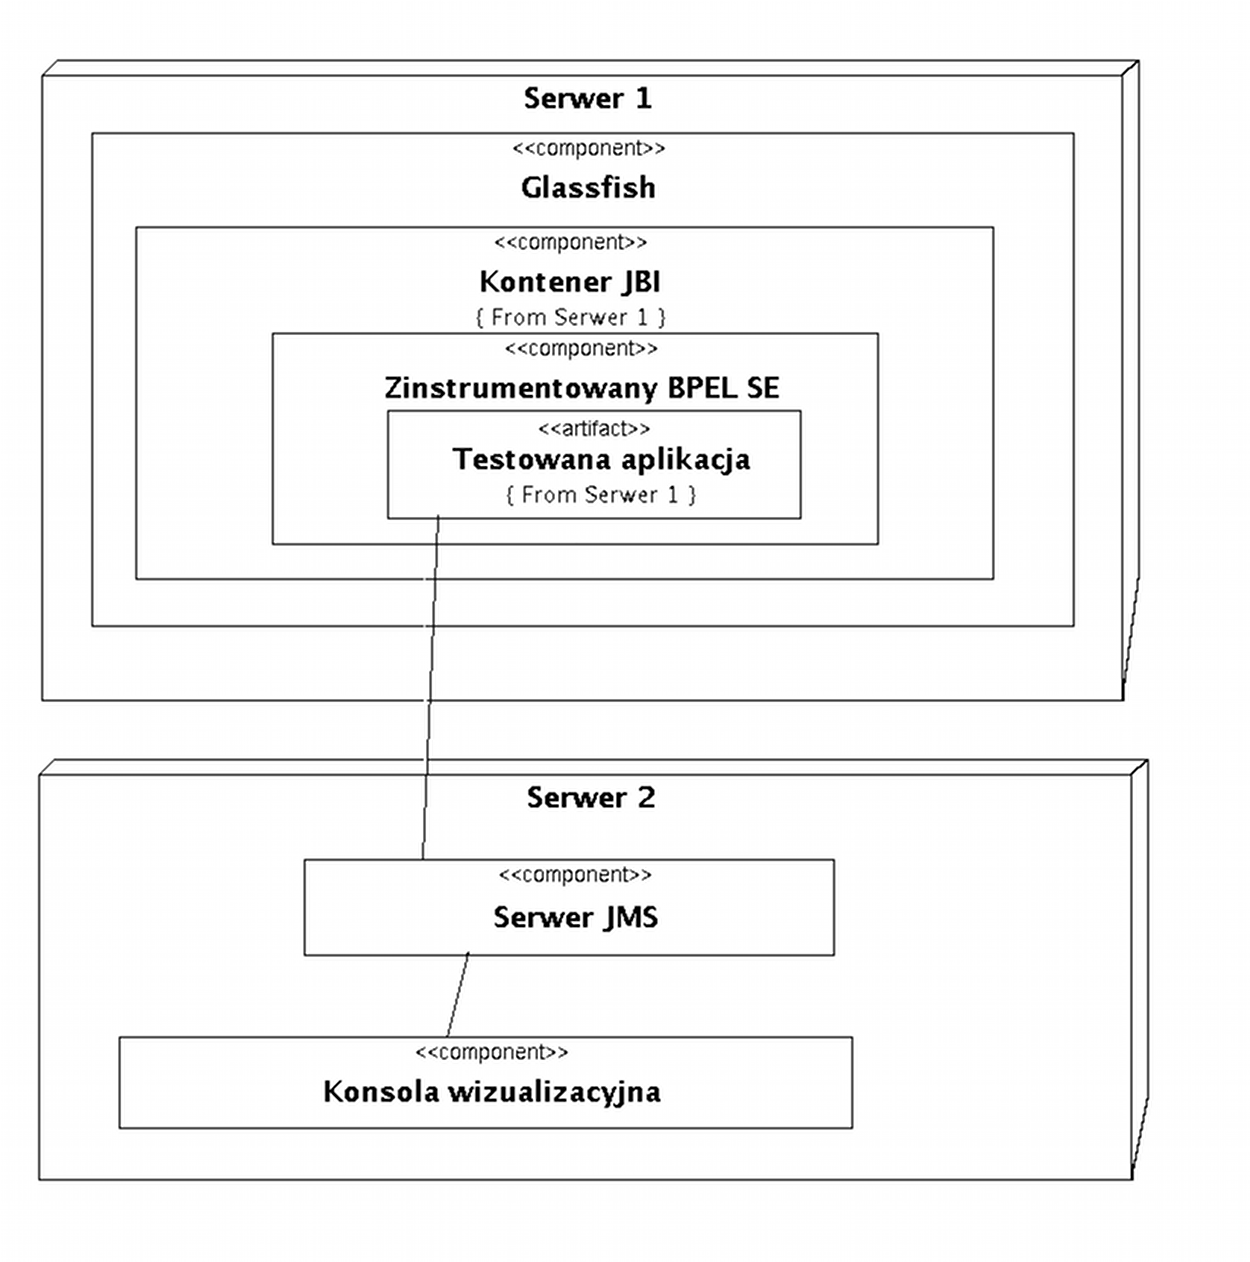
\includegraphics[bb=0 0 300 303]{tests/deployment.png}
 % deployment.png: 1250x1262 pixel, 300dpi, 10.58x10.68 cm, bb=0 0 300 303
 \caption{Diagram konfiguracji infrastruktury testowej}
 \label{fig:tests:deployment}
\end{figure}

Podczas konfiguracji zwr�cono szczeg�ln� uwag� na oddzielenie medium komunikacyjnego od �rodowiska zewn�trznego. Zosta�o ona ca�kowicie odizolowane, celem zniwelowania op�nie� i zak�oce� pracy ze strony innych komputer�w.

\paragraph{Konfiguracja oprogramowania} Zosta�a zainstalowana standardowa dystrybucja OpenESB w wersji \textit{v2-ur2-b04-patch-20080603}, uruchamiana na maszynie wirtualnej Java \textit{1.6.0\_03}. Konfiguracja sensora wydajno�ci oraz konsoli wizualizacyjnej zosta�a wykonana zgodnie z instrukcjami zawartymi w dodatku A.

\newpage

\section{Dynamiczna prezentacja wynik�w}

Konsola wizualizacyjna nie posiada informacji o oryginalnym modelu badanego procesu biznesowego. Model w konsoli jest budowany w spos�b dynamiczny, w miar� otrzymywania nowych informacji od sensora wydajno�ci. Przyk�ad dzia�ania mechanizmu dynamicznego budowania modelu procesu znajduje si� na rysunku \ref{fig:tests:diagram_grow}. Rysunek ilustruje badanie prostego procesu biznesowego, kt�ry sk�ada si� z wywo�ania operacji webservice (INVOKE) i ewentualnie obs�u�enia rzuconego wyj�tku. Na kolejnych fragmentach rysunku pokazono coraz bardziej uszczeg�owiony model procesu, kt�ry coraz lepiej przybli�a oryginalny model.

\newpage

\begin{figure}[htb!]
 \centering
 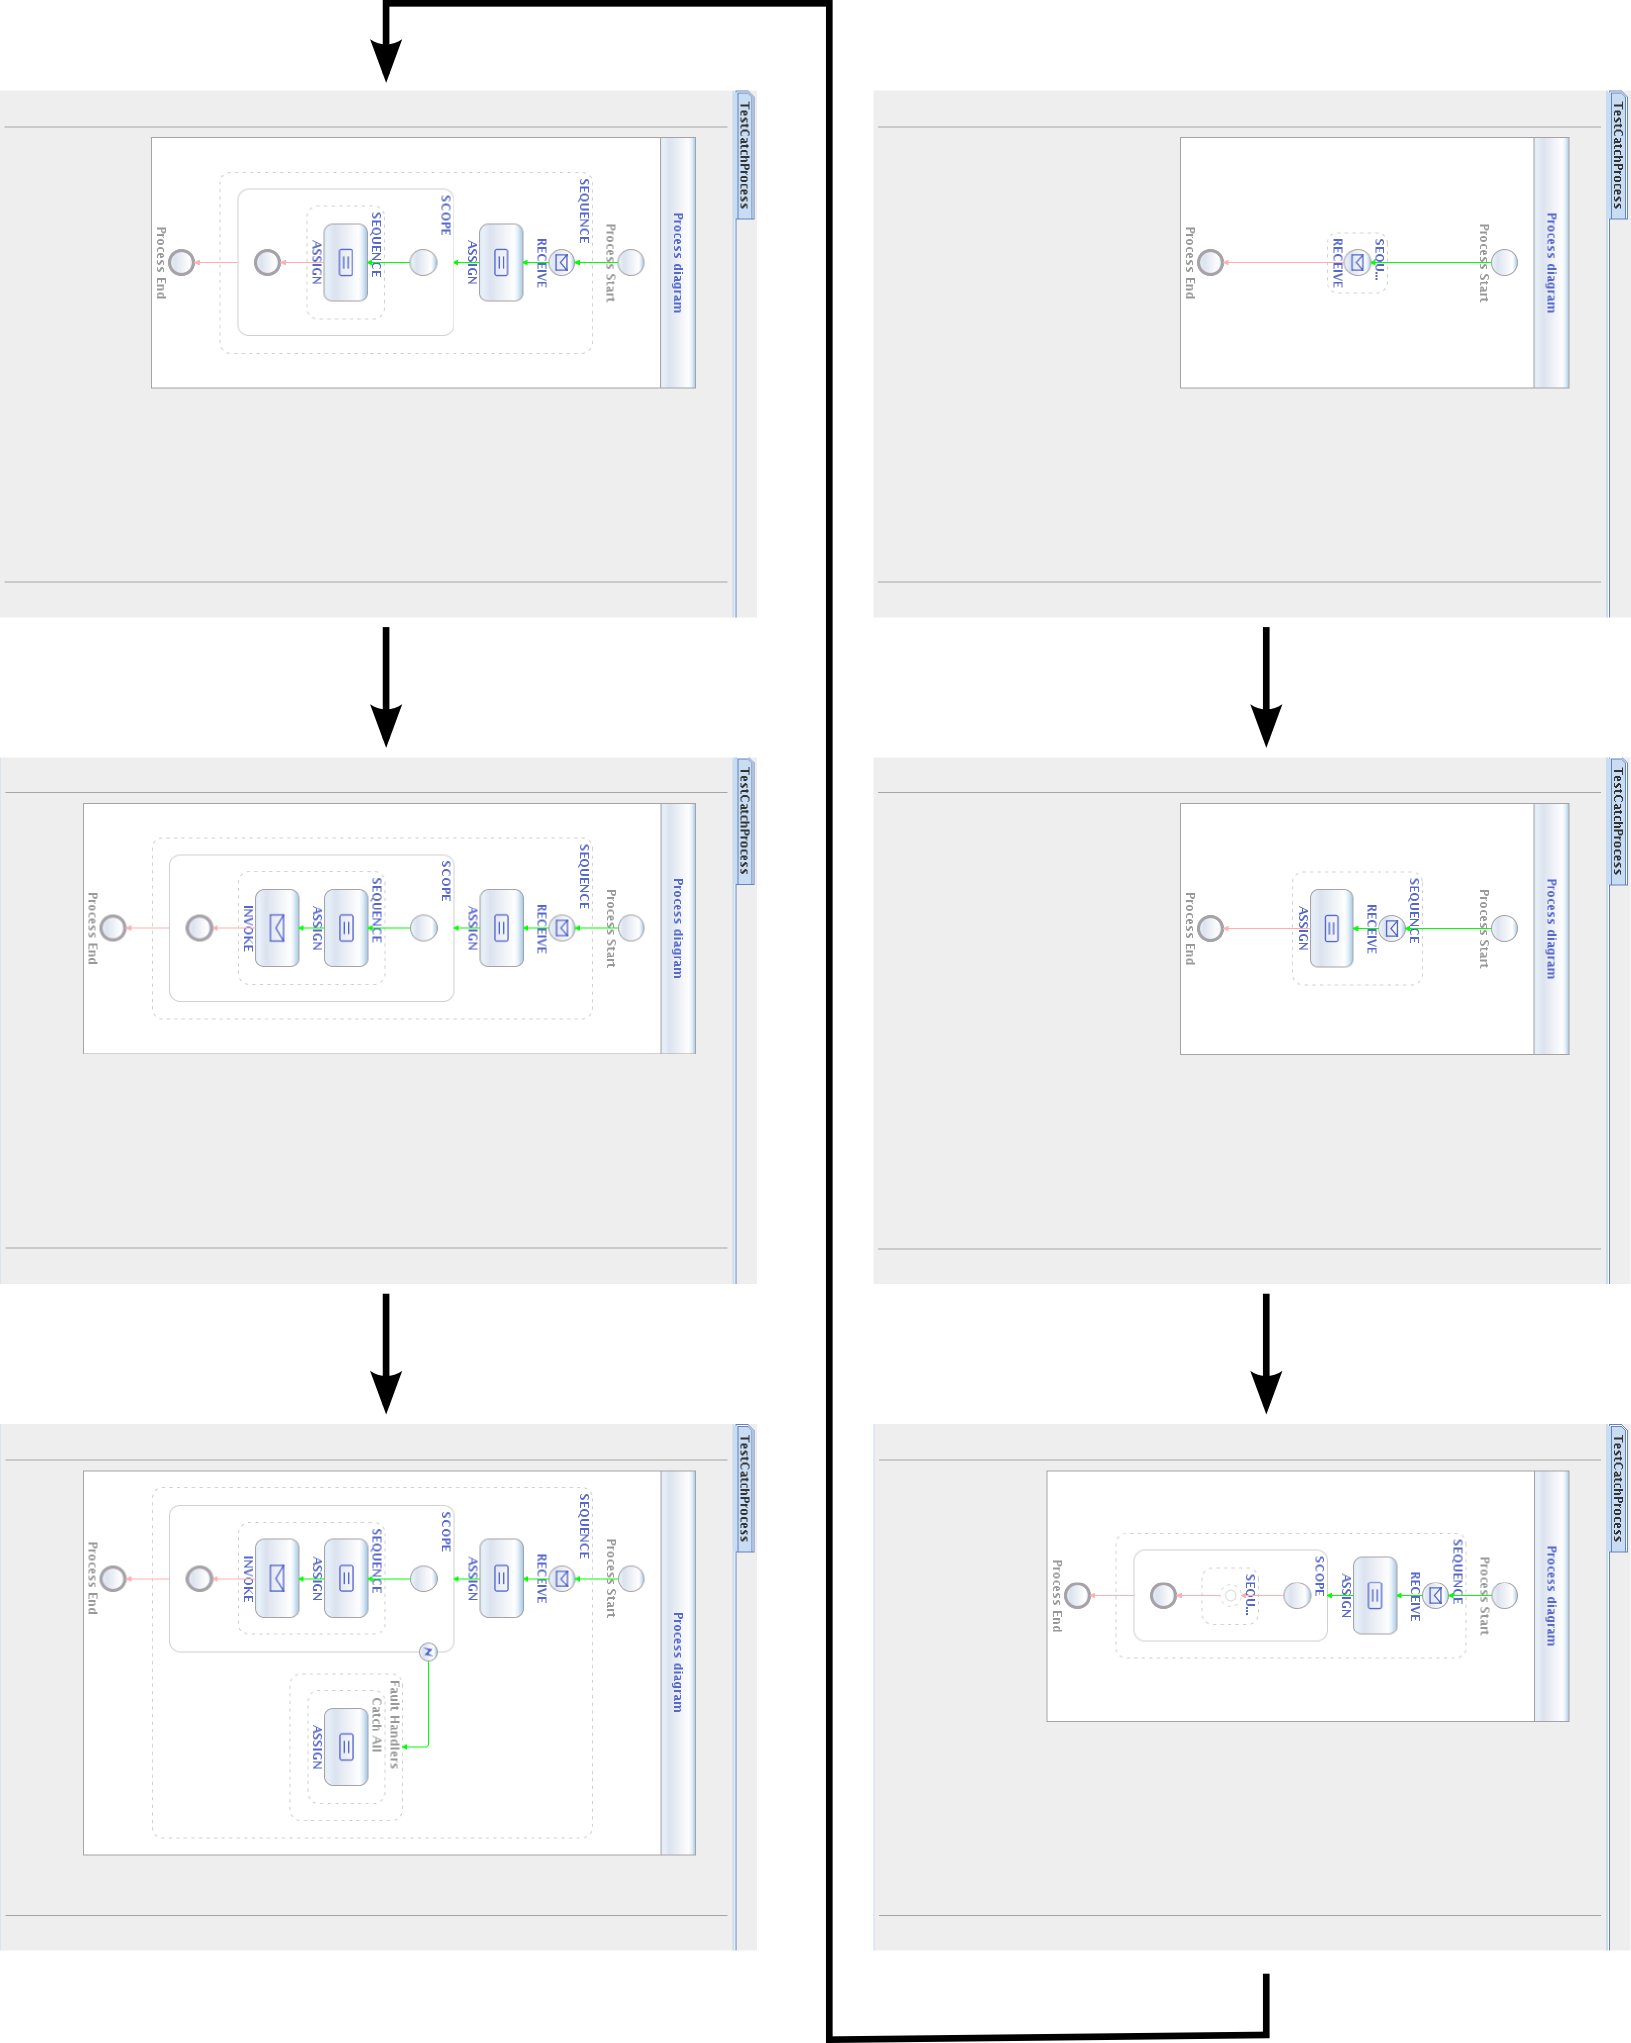
\includegraphics[bb=0 0 391 490]{ss/tests_diagram_grow2.png}
 % tests_diagram_grow2.png: 1631x2043 pixel, 300dpi, 13.81x17.30 cm, bb=0 0 391 490
 \caption{Dynamiczne budowanie modelu w trakcie zbierania danych}
 \label{fig:tests:diagram_grow}
\end{figure}


%Zrealizowana aplikacja w spos�b dynamiczny buduje model procesu, w miar� otrzymywania kolejnych danych. Mechanizm dynamicznego budowania modelu zosta� zilustrowany na rysunku \ref{fig:tests:diagram_grow}. Rysunek obrazuje dwukrotne wykonanie pewnego procesu biznesowego. Przy pierwszym wykonaniu procesu wybrana zosta�a lewa ga��� instrukcji IF, natomiast przy drugim wykonaniu prawa ga��� instrukcji IF (odpowiadaj�ca konstrukcji ELSE). Po pierwszym wykonaniu procesu konsola nie ma informacji o aktywno�ci zawartej w konstrukcji ELSE, dlatego prawe odga��zienie konstrukcji IF pozostaje puste (widoczne jest to na lewej cz�ci rysunku \ref{fig:tests:diagram_grow}. Przy drugim uruchomieniu procesu konsola uzyskuje informacje o aktywno�ci zawartej w konstrukcji ELSE i mo�e pokaza� pe�n� budow� u�ytej instrukcji warunkowej (por. prawa cz�� rysunku).

%\begin{figure}[htb!]
% \centering
% 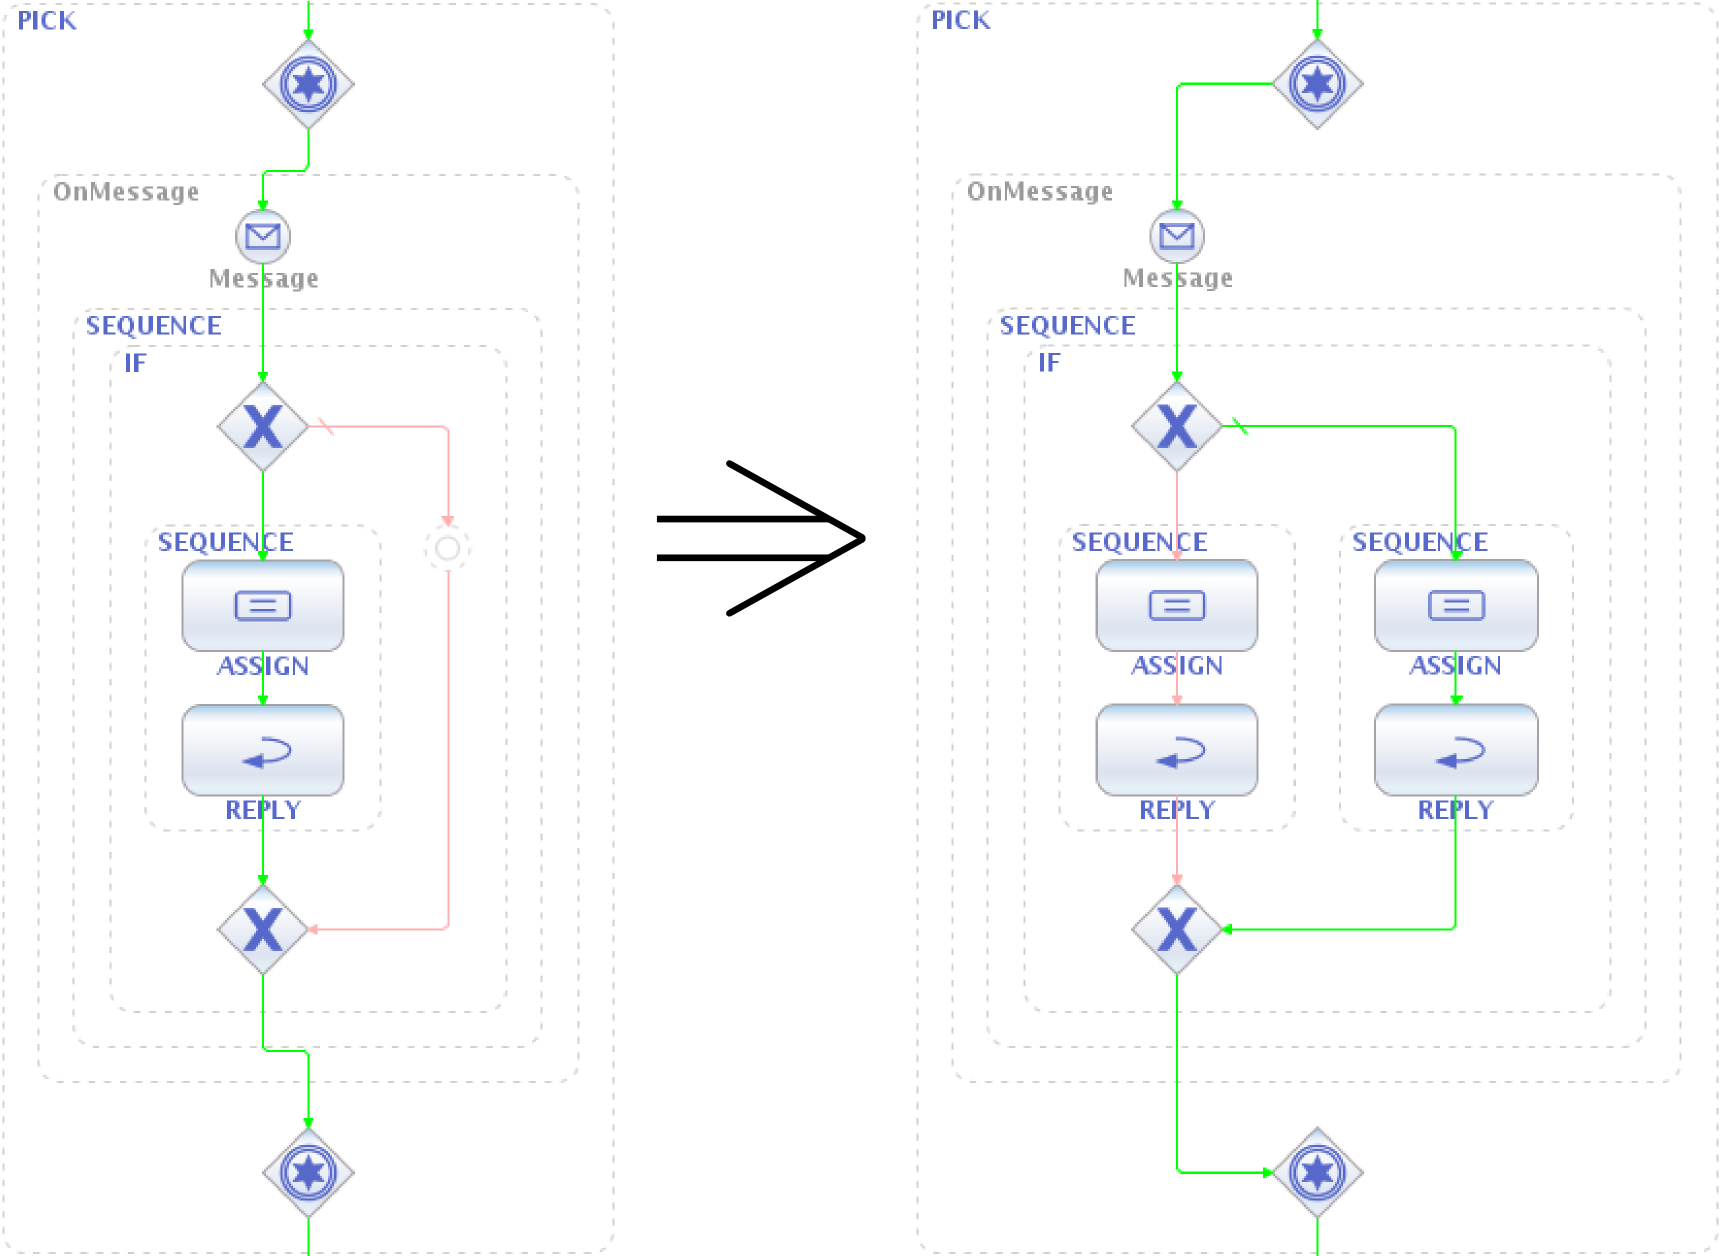
\includegraphics[bb=0 0 413 301]{ss/tests_diagram_grow.png}
% % tests1.png: 1720x1256 pixel, 300dpi, 14.56x10.63 cm, bb=0 0 413 301
% \caption{Dynamiczne budowanie modelu w trakcie zbierania danych}
% \label{fig:tests:diagram_grow}
%\end{figure}

\newpage

\section{Wyniki test�w}

Ka�da z aplikacji zaprezentowanych w rozdziale 5.1 zosta�a umieszczona w kontenerze. Procesy biznesowe oferowane przez aplikacje zosta�y kilkukrotnie wykonane (w miar� mo�liwo�ci starano si� pokaza� r�ne �cie�ki w procesach).  Wizualna weryfikacja otrzymanych rysunk�w pozwala stwierdzi�, �e s� one zgodne z oryginalnymi modelami proces�w biznesowych przedstawionymi w rozdziale 5.1. Otrzymane warto�ci liczbowe s� warto�ciami realistycznymi (brak konkurencyjnych narz�dzi uniemo�liwia przeprowadzenie test�w por�wnawczych). Dodatkowo w celu u�atwienia interpretacji otrzymanych wynik�w, na rysunku \ref{fig:tests_ss_overview} zamieszczono uk�ad i oznaczenie element�w g��wnego okna konsoli wizualizacyjnej.

\begin{figure}[htb!]
 \centering
 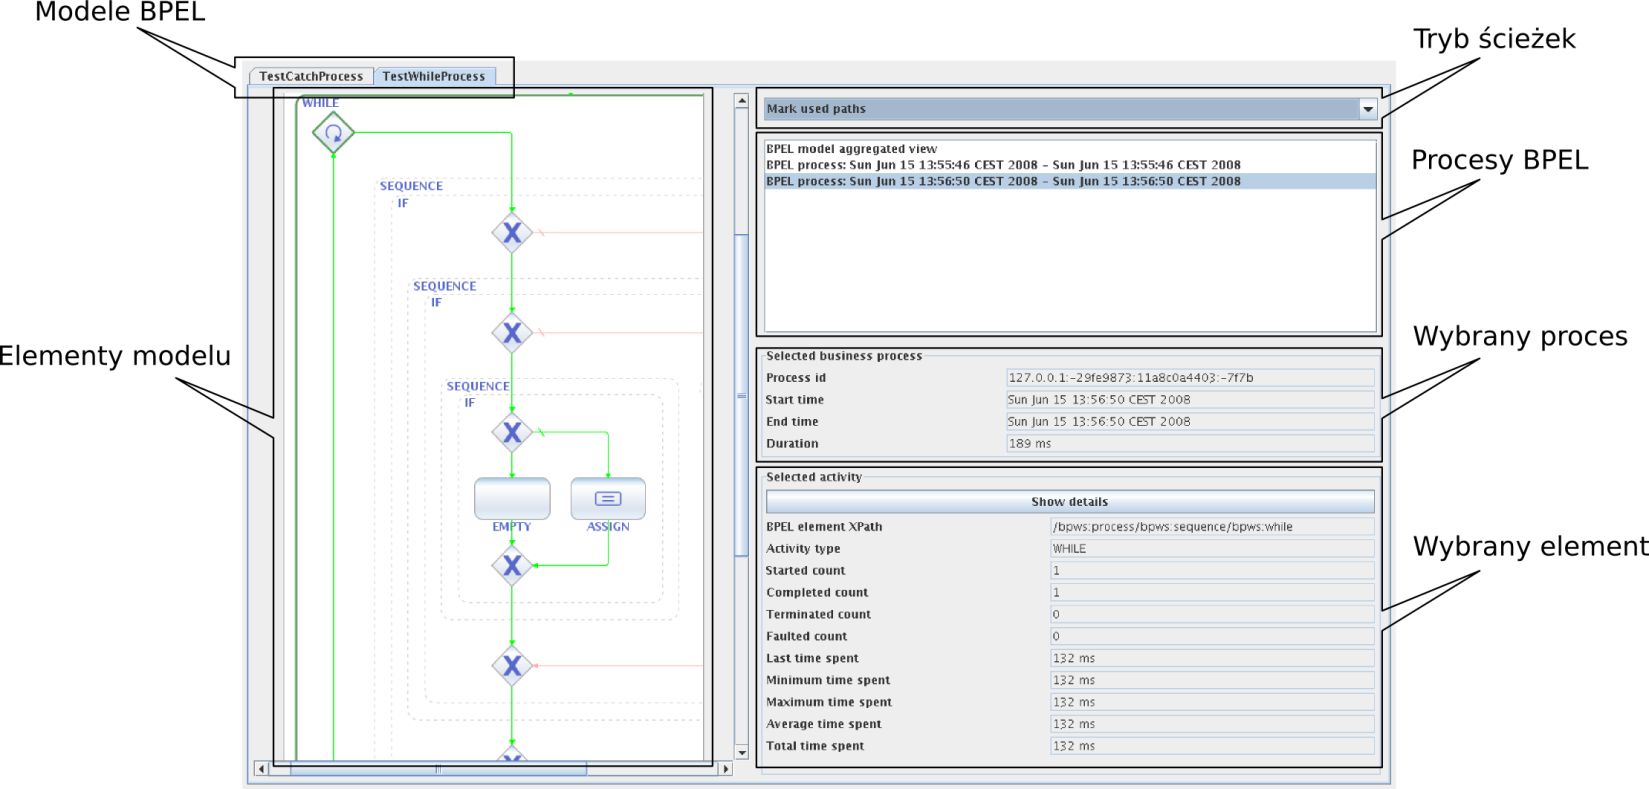
\includegraphics[bb=0 0 396 189]{appendix/ss_overview_small.png}
 % ss_overview.png: 1649x789 pixel, 300dpi, 13.97x6.68 cm, bb=0 0 396 189
 \caption{Uk�ad g��wnego okna aplikacji}
 \label{fig:tests_ss_overview}
\end{figure}

Zebrane dane zosta�y zaprezentowane na kolejnych stronach. Poni�ej znajduje si� kr�tki komentarz do ka�dego badanego procesu biznesowego.

\paragraph{Aplikacja realizuj�ca synchroniczne wywo�anie us�ugi}
Na rysunku \ref{fig:tests:ss_blueprint1} przedstawiono zagregowany widok modelu procesu po siedmiokrotnym wykonaniu procesu biznesowego. Zagregowany widok modelu pokazuje informacj� uzyskan� ze wszystkich wykona� procesu, dlatego w instrukcji IF pokazane zosta�y obie mo�liwo�ci wykonania (lewa ga��� wykonywana przy spe�nieniu warunku z instrukcji IF, prawa ga��� w przeciwnym razie).

\paragraph{Aplikacja realizuj�ca asynchroniczne wywo�anie us�ugi}
Rysunek \ref{fig:tests:ss_blueprint2} przedstawia fragment modelu demonstruj�cy u�ycie instrukcji IF. Analizuj�c �cie�k� wykonania mo�na zauwa�y�, �e zosta�a wykonana prawa cz�� instrukcji warunkowej odpowiadaj�ca za klauzul� ELSE.

\paragraph{Aplikacja realizuj�ca synchroniczne wywo�anie us�ugi z obs�ug� wyj�tk�w}

Rysunek \ref{fig:tests:ss_blueprint3} przedstawia proces realizacji b��dnego zam�wienia. Instrukcja IF (por. rysunek) odpowiada za zweryfikowanie typu zam�wienia. Poniewa� u�yty typ zam�wienia by� niepoprawny nast�puje przej�cie do instrukcji THROW, kt�ra generuje wyj�tek typu CannotCompleteOrder (prawy dolny r�g rysunku). Warto zauwa�y�, �e �cie�ka wychodz�ca z instrukcji THROW nie ma koloru oznaczaj�cego aktywno�� (zielonego), poniewa� sterowanie wskutek wyj�tku zostaje przeniesione bezpo�rednio do bloku obs�ugi wyj�tku CATCH. Obs�uga wyj�tku poprzez instrukcj� REPLY ustawia odpowiedni rezultat procesu biznesowego informuj�cy o nieprawid�owym zam�wieniu.

Rysunek \ref{fig:tests:ss_blueprint3_2} przedstawia proces realizacji zam�wienia niedost�pnego w magazynie. Typ zam�wienia zosta� pozytywnie zweryfikowany z u�yciem instrukcji warunkowej IF. Sterowanie zosta�o nast�pnie przekazane do instrukcji INVOKE, kt�ra wykonuje operacje webservice odpowiadaj�c� za sprawdzenie stanu magazynowego pod k�tem z�o�onego zam�wienia. Poniewa� w magazynie brakuje zamawianych towar�w, wywo�anie operacji ko�czy si� wyj�tkiem InventoryFaultType (prawy dolny r�g rysunku).

Przyk�adowe statystyki wykonania operacji INVOKE pokazano na rysunku \ref{fig:tests:ss_blueprint3_details}. W drugim wierszu mo�na zauwa�y� niepoprawne zako�czenie operacji INVOKE wskutek wyst�pienia wyj�tku InventoryFaultType (wyj�tek ten oznacza� brak zamawianych towar�w w magazynie).

\paragraph{Aplikacja koreluj�ca kilka wywo�a�}
Rysunek \ref{fig:tests:ss_blueprint4} przedstawia fragment modelu demonstruj�cy u�ycie instrukcji PICK. Analizuj�c �cie�k� wykonania mo�na zauwa�y�, �e proces po napotkaniu instrukcji PICK zatrzyma� si� w oczekiwaniu na dowolny z dw�ch typ�w komunikat�w (obszary OnMessage). Funkcjonalno�� ta jest wykorzystywana do zrealizowania mo�liwo�ci anulowania lub potwierdzania z�o�onego zam�wienia. Po otrzymaniu komunikatu z potwierdzeniem zam�wienia nast�pi�o dalsze wykonanie procesu. 

\paragraph{Aplikacja realizuj�ca r�wnoleg�e asynchroniczne wywo�anie kilku us�ug}
Rysunek \ref{fig:tests:ss_blueprint5} przedstawia wykonywanie r�wnoleg�ej rezerwacji biletu lotniczego, hotelu oraz samochodu. Fragmenty odpowiadaj�ce za obs�ug� rezerwacji hotelu oraz samochodu zosta�y zwini�te, wskutek czego zajmuj� mniej miejsca oraz uwydatniaj� pozosta�� cz�� modelu.

%Z uwagi na charakter pracy, przedstawione wyniki stanowi� jedynie efekt dzia�ania stworzonego oprogramowania. Analiza wynik�w nie zosta�a uj�ta w obr�bie niniejszej pracy.

\newpage

\begin{figure}[htb!]
 \centering
 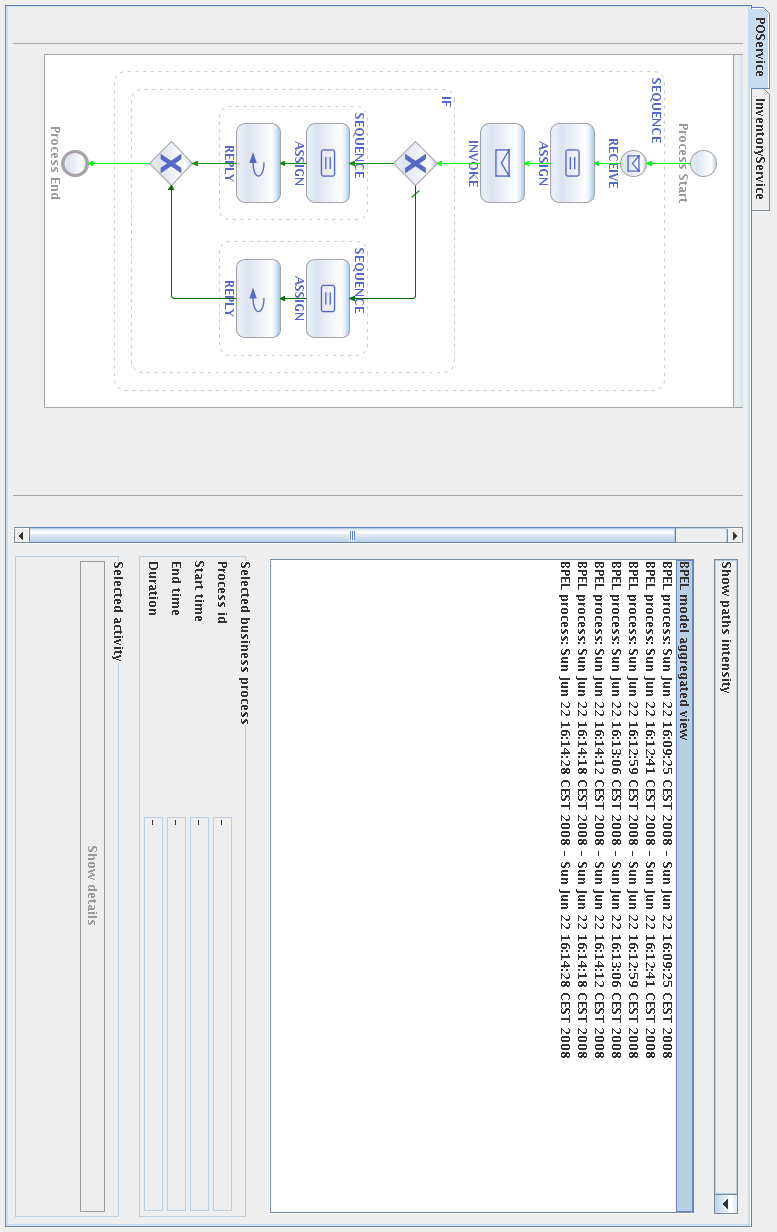
\includegraphics[bb=0 0 320 507]{ss/blueprint1.png}
 % blueprint1.png: 777x1232 pixel, 175dpi, 11.28x17.88 cm, bb=0 0 320 507
 \caption{Aplikacja realizuj�ca synchroniczne wywo�anie us�ug (por. rysunek 5.1).}
 \label{fig:tests:ss_blueprint1}
\end{figure}

\newpage

\begin{figure}[htb!]
 \centering
 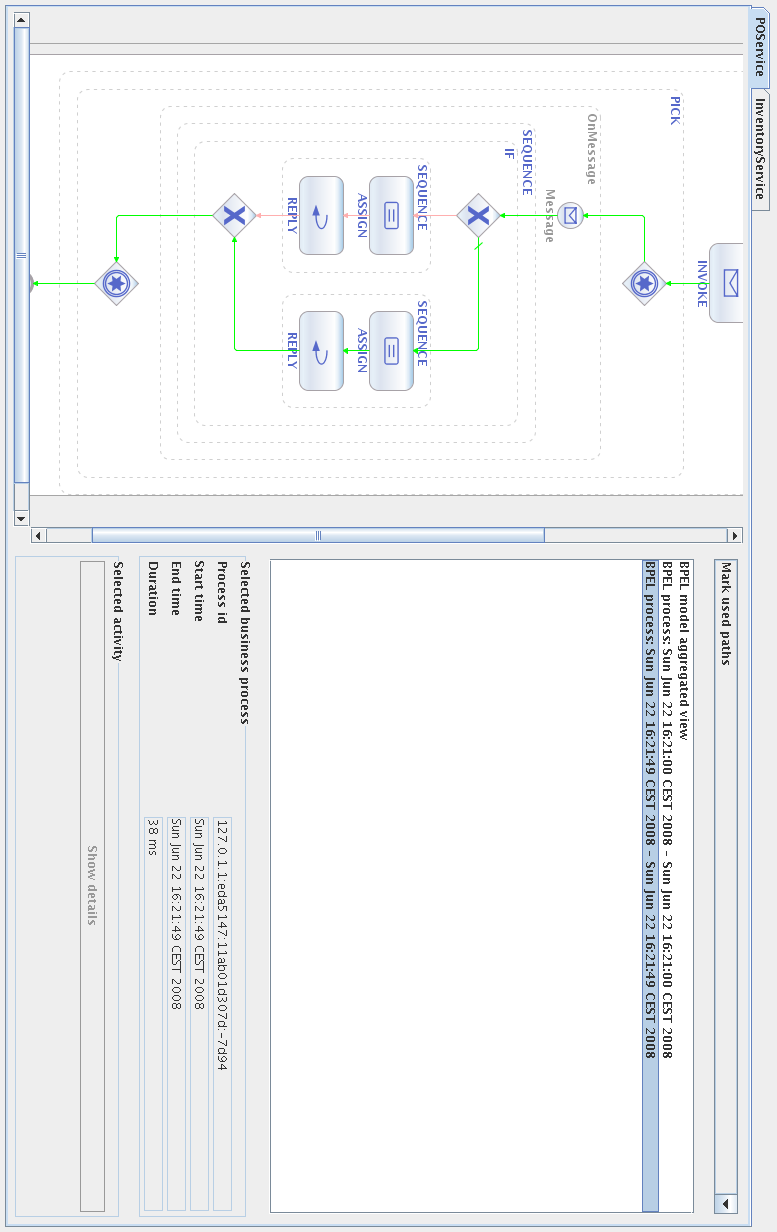
\includegraphics[bb=0 0 320 507]{ss/blueprint2.png}
 % blueprint2.png: 777x1232 pixel, 175dpi, 11.28x17.88 cm, bb=0 0 320 507
 \caption{Aplikacja realizuj�ca asynchroniczne wywo�anie us�ugi (por. rysunek 5.2).}
 \label{fig:tests:ss_blueprint2}
\end{figure}

\newpage

\begin{figure}[htb!]
 \centering
 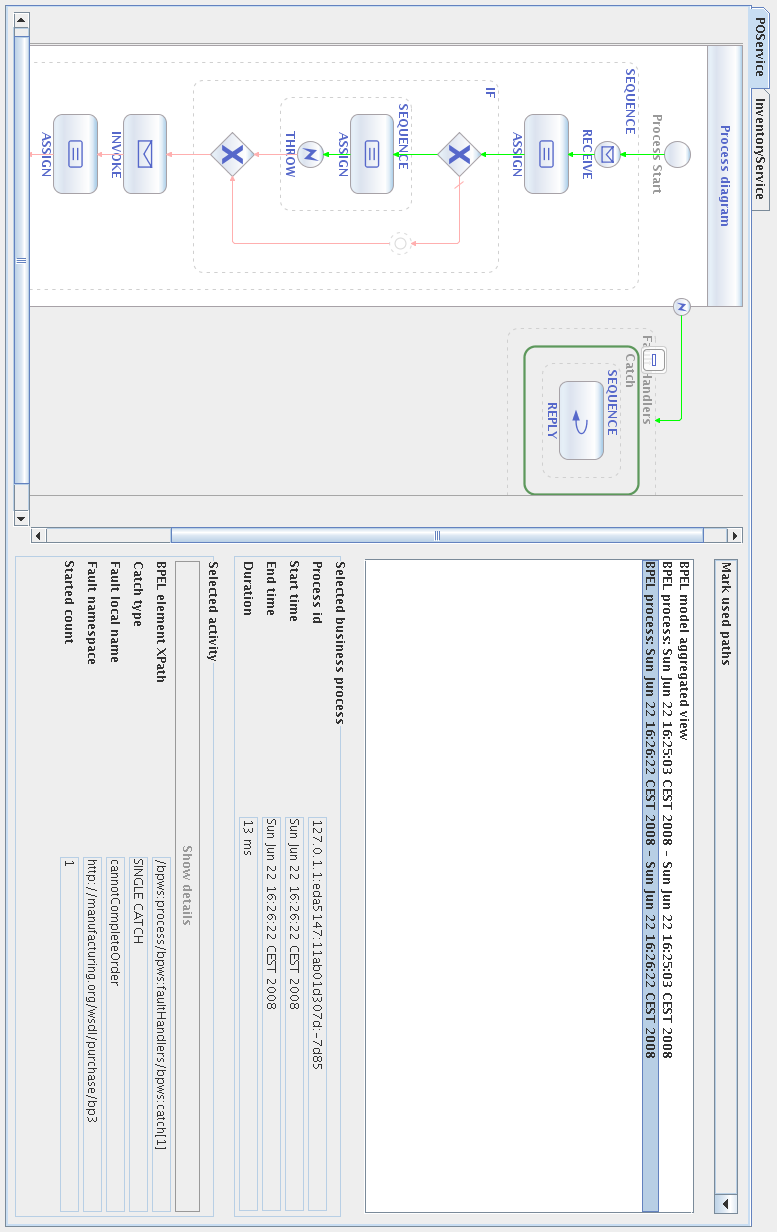
\includegraphics[bb=0 0 320 507]{ss/blueprint3.png}
 % blueprint3.png: 777x1232 pixel, 175dpi, 11.28x17.88 cm, bb=0 0 320 507
 \caption{Aplikacja realizuj�ca synchroniczne wywo�anie us�ugi z obs�ug� wyj�tk�w (por. rysunek 5.3).}
 \label{fig:tests:ss_blueprint3}
\end{figure}

\newpage

\begin{figure}[htb!]
 \centering
 \includegraphics[bb=0 0 320 507]{ss/blueprint3_2.png}
 % blueprint3.png: 777x1232 pixel, 175dpi, 11.28x17.88 cm, bb=0 0 320 507
 \caption{Aplikacja realizuj�ca synchroniczne wywo�anie us�ugi z obs�ug� wyj�tk�w (por. rysunek 5.3).}
 \label{fig:tests:ss_blueprint3_2}
\end{figure}

\newpage

\begin{figure}[htb!]
 \centering
 \includegraphics[bb=0 0 231 480]{ss/blueprint3_details.png}
 % blueprint3_details.png: 481x1000 pixel, 150dpi, 8.14x16.93 cm, bb=0 0 231 480
 \caption{Szczeg�y dzia�ania aktywno�ci INVOKE z rysunku 5.10.}
 \label{fig:tests:ss_blueprint3_details}
\end{figure}

\newpage

\begin{figure}[htb!]
 \centering
 \includegraphics[bb=0 0 320 507]{ss/blueprint4.png}
 % blueprint4.png: 777x1232 pixel, 175dpi, 11.28x17.88 cm, bb=0 0 320 507
 \caption{Aplikacja koreluj�ca kilka wywo�a� (por. rysunek 5.4).}
 \label{fig:tests:ss_blueprint4}
\end{figure}

\newpage

\begin{figure}[htb!]
 \centering
 \includegraphics[bb=0 0 320 507]{ss/blueprint5.png}
 % blueprint5.png: 777x1232 pixel, 175dpi, 11.28x17.88 cm, bb=0 0 320 507
 \caption{Aplikacja realizuj�ca r�wnoleg�e asynchroniczne wywo�anie kilku us�ug (por. rysunek 5.5).}
 \label{fig:tests:ss_blueprint5}
\end{figure}


\newpage

Wykazano przydatno�� stworzonego narz�dzia w pomiarach wydajno�ci aplikacji o architekturze SOA. Oprogramowanie dzia�a�o poprawnie - prezentowane przej�cia w procesach biznesowych pokrywa�y si� z rzeczywisto�ci�. Wyniki test�w wydajno�ciowych by�y zgodne z oczekiwaniami, co oznacza, �e narz�dzie mo�e by� z powodzeniem u�yte w analizie wydajno�ci aplikacji.

% Wyniki b�d�ce efektem dzia�ania programu mog� stanowi� podstaw� do szerokiej analizy wydajno�ci,  r�wnie� poszukiwanie tzw. ``w�skich garde�''. Mo�liwo�� obserwacji cz�sto�ci przej�� proces�w przez poszczeg�lne aktywno�ci procesu, umo�liwia wyodr�bnienie najcz�stszych przypadk�w u�ycia. 

% Przeprowadzenie takiej analizy pomini�to, gdy� wykracza to poza ramy pracy.



% \part{Zako�czenie}

\chapter{Wnioski z pracy i mo�liwo�ci dalszego rozwoju systemu}

SOA to wci�� innowacyjny paradygmat tworzenia oprogramowania.
Ju� teraz mo�na jednak zaobserwowa� tendencj� do zwi�kszania si� jego udzia�u w�r�d aktualnie dominuj�cych technologii IT.
Coraz wi�cej system�w opartych jest o paradygmat SOA, co przynosi wymierne korzy�ci w postaci np. lu�nych powi�za� pomi�dzy us�ugami, ich u�atwionej integracji oraz konieczno�ci stosowania kontrakt�w.
Badanie wydajno�ci us�ug realizuj�cych procesy biznesowe z u�yciem j�zyka BPEL jest bardzo przydatne, poniewa� pozwala m.in. znale�� s�abe punkty tworzonej aplikacji (ang. bottlenecks), analizowa� zachowanie si� konkretnych wywo�a� proces�w biznesowych oraz wyszukiwa� b��dy i niepoprawnie dzia�aj�ce procesy.
Autorom niniejszej pracy w trakcie jej tworzenia nie uda�o si� znale�� aplikacji wspieraj�cych takie badania oraz spe�niaj�cych jednocze�nie zbi�r wymaga� zawartych w rozdziale 3.1.
Autorzy zaproponowali modularn� architektur� aplikacji pozwalaj�c� analizowa� procesy biznesowe zachodz�ce w dowolnym kontenerze aplikacji oraz obrazowa� je w czytelny spos�b z u�yciem centralnej konsoli wizualizacyjnej.

W ramach pracy autorzy zapoznali si� z mo�liwo�ciami technologii wspomagaj�cych budowanie aplikacji o architekturze SOA. Pog��biona zosta�a wiedza na temat j�zyka BPEL i rozwi�za� realizuj�cych koncepcj� ESB. Wyniki analizy mo�liwo�ci oprogramowania wspieraj�cego tworzenie rozwi�za� o architekturze SOA, zosta�y wykorzystane do wybrania przyk�adowego, testowanego �rodowiska.
% W rezultacie naszej pracy mamy mo�liwo�� ????. (zdania magisterki :)

Postawione zosta�y wymagania jakie powinien spe�nia� system badania wydajno�ci, ze szczeg�lnym naciskiem na spos�b umieszczenia sensora w obr�bie �rodowiska wykonawczego.
% Rozwa�ono kilka koncepcji, i wybrano do implementacji najlepiej pasuj�c� w kontek�cie postawionych wymaga�.
Za zbioru rozwa�anych koncepcji, do implementacji wybrano najlepiej pasuj�c� w kontek�cie postawionych wymaga�.

Stworzone zosta�o zar�wno narz�dzie do automatycznej instrumentacji �rodowiska wykonawczego, jak i obserwacji otrzymywanych parametr�w wydajno�ciowych aplikacji.
Zosta�o ono wzbogacone o mo�liwo�� przedstawiania wynik�w obserwacji w postaci samobuduj�cego si� procesu biznesowego.

W celu prezentacji osi�gni�� przygotowane zosta�o �rodowisko testowe.
Do testowania wybrano kilka przyk�adowych aplikacji, realizuj�cych typowe przypadki u�ycia w aplikacjach opartych o j�zyk BPEL. 
Przypadki te by�y podstaw� do przeprowadzenia procedur testowych, oraz �r�d�em zamieszczonych w pracy wynik�w.
% W oparciu o powy�sze przeprowadzono przyk�adow� procedur� testow�, b�d�c� �r�d�em zamieszczonych w pracy wynik�w.

\section{Mo�liwo�ci zastosowania stworzonego oprogramowania}

Stworzone oprogramowanie w pe�ni spe�nia postawione w pracy wymagania.
Narz�dzie pozwala na wykonanie pomiar�w dzia�aj�cej aplikacji, bez znacznej ingerencji w �rodowisko wykonawcze. Dostarczane statystyki s� zbierane w locie z dowolnej liczby kontener�w i wysy�ane w og�lnie znanym formacie do serwera JMS, dzi�ki czemu mo�liwa jest ich jednoczesna analiza w kilku lokalizacjach.

Narz�dzie wizualizacyjne pozwala na prezentacj� wynik�w analizy w trakcie dzia�ania aplikacji, pozwalaj�c jednocze�nie na szybkie odnalezienie ``w�skich garde�'' system�w. Zbierane statystyki mo�na poddawa� dalszej obr�bce, celem dalszej agregacji, tworzeniu wykres�w itp. Z uwagi na niski narzut czasowy wprowadzany instrumentacj� �rodowiska wykonawczego, narz�dzie mo�e by� z powodzeniem stosowane w dzia�aj�cych aplikacjach m.in. do �ledzenia cz�sto�ci przej�� poszczeg�lnych �cie�ek w procesie biznesowym.

Dzi�ki intuicyjnemu interfejsowi u�ytkownika, narz�dzie mo�e by� u�ywane nawet przez programist�w o niewielkiej wiedzy w dziedzinie problemu. Nieskomplikowana forma prezentacji graficznej wynik�w pomiar�w, pozwala na przedstawianie ich osobom nie posiadaj�cym szczeg�owej wiedzy technicznej.

\section{Dalszy rozw�j systemu}

Zrealizowana aplikacja ma s�u�y� jako przyk�adowe rozwi�zanie problemu badania wydajno�ci us�ug zgodnych z paradygmatem SOA. Aplikacja nie powinna by� wi�c traktowana jako kompletny program, lecz jako punkt wyj�cia do dalszych prac i udoskonale�.

\paragraph{Zwi�kszenie ilo�ci obs�ugiwanych implementacji}

Aplikacja zosta�a wyposa�ona w regu�y instrumentacji kontener�w OpenESB. Poniewa� sama aplikacja ma jedynie demonstrowa� spos�b badania wydajno�ci, wi�c ograniczenie wbudowanej obs�ugi kontener�w tylko do OpenESB nie ma wp�ywu na testy opisane w rozdziale 5. Modu�owa budowa sensora wydajno�ci umo�liwia proste dopisanie regu� instrumentacji dla dowolnego kontenera ESB. Regu�y te s� podstaw� do dokonania instrumentacji przez bibliotek� wstrzykuj�c� kod (por. rozdzia� 4.1.1). Biblioteka ta zapewnia podstawowy zestaw adnotacji dla pisania regu� (np. wykonaj podany kod przed startem okre�lonej metody). Zestaw ten mo�e by� poszerzony w przypadku braku odpowiedniej adnotacji. W szczeg�lnych przypadkach istnieje mo�liwo�� wymiany ca�ego silnika instrumentuj�cego kod, bez zmiany pozosta�ej cz�ci systemu (konsoli, sensor�w, formatu wiadomo�ci JMS itp). Kolejnym etapem pracy nad aplikacj� powinno by� napisanie regu� instrumentacji dla najpopularniejszych kontener�w obecnych na rynku.
W przypadku u�ywania platformy OSGi\cite{concl:osgi} (system modu��w dla j�zyka Java) bezpo�rednie wsparcie dla j�zyka BPEL b�dzie umo�liwia�a nowa wersja serwera GlassFish 3.0\cite{concl:glassfishv3}. Poniewa� regu�y instrumentacji OpenESB s� ju� utworzone, mamy mo�liwo�� badania i analizowania wydajno�ci us�ug zrealizowanych z u�yciem j�zyka BPEL w dowolnym �rodowisku OSGi.


\paragraph{Rozszerzenie mo�liwo�ci wizualizacyjnych konsoli}

Obecnie konsola wizualizacyjna jest w stanie przedstawi� badany proces w postaci diagramu BPEL. Posiada r�wnie� mo�liwo�� wy�wietlania informacji statystycznych (np. statystyki czasowe czyli minimalny, �redni i maksymalny czas trwania aktywno�ci) o dowolnym elemencie procesu. Otrzymywane od sensor�w dane pozwalaj� jednak na prezentacj� wi�kszej ilo�ci informacji. Pozwalaj� one np. na wykre�lanie diagram�w Gantta\cite{diagram:gantt} zachodz�cego procesu. Obrazuje on podzia� procesu na poszczeg�lne zadania oraz rozmieszczenie ich w czasie. Dodatkowo obecn� wersj� aplikacji mo�na rozszerzy� o mo�liwo�� rysowania wykres�w (np. koszt wywo�ania operacji webservice w czasie).

\paragraph{Integracja prezentacji wynik�w z modu�em NetBeans BPEL Designer}

�rodowisko programowania NetBeans udost�pnia wbudowany modu� BPEL Designer umo�liwiaj�cy graficzn� edycj� i modelowanie proces�w BPEL. Fragmenty tego modu�u zosta�y u�yte w stworzonej przez autor�w aplikacji do prezentowania procesu BPEL w konsoli wizualizacyjnej. Docelowo nale�a�oby r�wnie� zrealizowa� integracj� w drug� stron�, czyli wbudowa� w edytor Netbeans BPEL Designer mo�liwo�ci konsoli wizualizacyjnej proces�w BPEL. Posiadanie danych o wydajno�ci budowanego procesu bezpo�rednio w edytorze, usprawni�oby modelowanie proces�w, oraz umo�liwi�o efektywniejsze i szybsze poprawianie b��d�w w ich modelach.

\bigskip

Niniejsza praca magisterska wpisuje si� w aktualne �wiatowe trendy tworzenia aplikacji opartych o us�ugi i stara si� wype�ni� luk� w badaniu ich wydajno�ci.
Stworzone oprogramowanie stanowi solidne narz�dzie niezb�dne do produkcyjnego zastosowania procedur biznesowych implementowanych w oparciu o j�zyk BPEL.
Mnogo�� postawionych w pracy problem�w oraz mo�liwo�ci rozwoju stworzonego oprogramowania, �wiadczy o szerokim spektrum mo�liwych kontynuacji bada� w tej dziedzinie.


\chapter{Akronimy}

\begin{itemize}
%  \item AOP - Aspect Oriented Programming
%  \item JVM - Java Virtual Machine
%  \item CORBA - Common Request Object Broker Architecture
%  \item DCOM - Distributed Component Object Model
%  \item RMI - Remote Method Invocation
%  \item JMS - Java Message Service
%  \item RPC - Remote Procedure Call
%  \item IIOP - Internet Inter Orb Protocol
%  \item BPM - Business Process Management
%  \item WS - WebService
%  \item ESB - Enterprise Service Bus
%  \item p2p - peer to peer
%  \item SOA - Service Oriented Architecture
%  \item BPEL - Business Process Execution Language
%  \item XML - eXtensible Markup Language
%  \item EAI - Enterprise Application Integration
%  \item EII - Enterprise Information Integration
%  \item MOM - Message Oriented Middleware
%  \item QoS - Quality of Service
%  \item SLA - Service Level Agreement
%  \item BPEL - Business Process Execution Language
%  \item JBI - Java Business Integration
%  \item BPEL4WS - Bussiness Process Execution Language for WebServices
%  \item WS-BPEL - WebServices - Bussiness Process Execution Language
%  \item JSR - Java Specification Request
%  \item JCP - Java Community Process
%  \item NMR - Normalized Message Router
%  \item SE - Service Engine
%  \item BC - Binding Component
%  \item SOAP - Service Oriented Architecture Protocol
%  \item UDDI - Universal Description, Discovery and Integration
%  \item WSDL - Web Service Definition Language
%  \item REST - Representational State Transfer
%  \item XSLT - eXtensible Stylesheet Language Tranformations
%  \item ETL - Extract, Transform and Load
%  \item XMPP - Extensible Messaging and Presence Protocol
 
 % after sort
 \item AOP - Aspect Oriented Programming
\item BC - Binding Component (JBI)
\item BPEL4WS - Bussiness Process Execution Language for WebServices
\item BPEL - Business Process Execution Language
\item BPEL - Business Process Execution Language
\item BPM - Business Process Management
\item CORBA - Common Request Object Broker Architecture
\item DCOM - Distributed Component Object Model
\item EAI - Enterprise Application Integration
\item EII - Enterprise Information Integration
\item ESB - Enterprise Service Bus
\item ETL - Extract, Transform and Load
\item IIOP - Internet Inter Orb Protocol
\item JBI - Java Business Integration
\item JCP - Java Community Process
\item JMS - Java Message Service
\item JSR - Java Specification Request
\item JVM - Java Virtual Machine
\item MOM - Message Oriented Middleware
\item NMR - Normalized Message Router
\item p2p - peer to peer
\item QoS - Quality of Service
\item REST - Representational State Transfer
\item RMI - Remote Method Invocation
\item RPC - Remote Procedure Call
\item SE - Service Engine (JBI)
\item SLA - Service Level Agreement
\item SOAP - Service Oriented Architecture Protocol
\item SOA - Service Oriented Architecture
\item SU - Service Unit (JBI)
\item UDDI - Universal Description, Discovery and Integration
\item WS-BPEL - WebServices - Bussiness Process Execution Language
\item WSDL - Web Service Definition Language
\item WS - WebService
\item XML - eXtensible Markup Language
\item XMPP - Extensible Messaging and Presence Protocol
\item XSLT - eXtensible Stylesheet Language Tranformations
\end{itemize}


% ponizszy fragment umieszcza bibliografie w osobnym rozdziale oraz wylacza justyfikacje (viva la \LaTeX :)
\makeatletter
\def\thebibliography#1{\chapter{Bibliografia\@mkboth
	{REFERENCES}{REFERENCES}}\raggedright\list
	{[\arabic{enumi}]}{\settowidth\labelwidth{[#1]}\leftmargin\labelwidth
	\advance\leftmargin\labelsep
	\usecounter{enumi}}
\def\newblock{\hskip .11em plus .33em minus .07em}
\sloppy\clubpenalty4000\widowpenalty4000
\sfcode`\.=1000\relax}
\makeatother

\bibliographystyle{plain}
\bibliography{bibliography}

\makeatletter
\renewcommand\listoffigures{%
    \if@twocolumn
      \@restonecoltrue\onecolumn
    \else
      \@restonecolfalse
    \fi
    \chapter{Spis rysunk�w}%
      \@mkboth{SPISRYSUNKOW}%
              {SPISRYSUNKOW}%
    \@starttoc{lof}%
    \if@restonecol\twocolumn\fi
    }
\makeatother

\listoffigures

\appendix


\chapter{Podr�cznik u�ytkownika}

W niniejszym dodatku przedstawiony zosta� kr�tki opis konfiguracji oraz obs�ugi aplikacji. Opis zosta� przygotowany do u�ycia w systemach z rodziny Linux, jednak w analogiczny spos�b przebiega konfiguracja i obs�uga aplikacji w systemie Windows. Aplikacja zosta�a napisana i przetestowana w �rodowisku maszyny wirtualnej Java 1.6.0.

Pierwszym krokiem kt�ry nale�y wykona� przed u�ytkowaniem niniejszej aplikacji jest odpowiednie zinstrumentowanie bibliotek kontenera oraz konfiguracja aplikacji.

\section{Instrumentacja bibliotek kontenera oraz konfiguracja aplikacji}

W og�lnym przypadku komputery u�yte w badaniu wydajno�ci us�ug maj� nast�puj�ce nazwy symboliczne i przeznaczenie:
\begin{itemize}
 \item \textbf{host1} - serwer JMS
 \item \textbf{host2} - konsola wizualizacyjna z aplikacj� dost�pn� w katalogu \textit{~/app}
 \item \textbf{host3..hostN} - kontenery us�ug z zainstalowanym GlassFish w katalogu \textit{/opt/glassfish}
\end{itemize}
Mo�liwy jest te� wariant prostszy, w kt�rym \textbf{host1} oraz \textbf{host2} oznaczaj� ten sam komputer.

Aby zbada� wydajno�� us�ug przechowywanych w kontenerach, nale�y wykona� nast�puj�ce kroki:

\begin{enumerate}
 \item \textbf{Uruchomienie serwera JMS}

Na komputerze \textbf{host1} powinien zosta� uruchomiony serwer JMS. S�u�y on do przesy�ania wiadomo�ci pomi�dzy sensorami wydajno�ci oraz konsol�. Adres IP komputera \textbf{host1} powinien by� widoczny dla konsoli oraz wszystkich komputer�w na kt�rych zostan� umieszczone kontenery us�ug. Nale�y pami�ta� o ustawieniu w polu \textit{ServerConfiguration} adresu IP komputera \textbf{host1} w pliku \textit{openjms.xml} z katalogu \textit{openjms/config}. Serwer JMS uruchamiany jest skryptem \textit{startup.sh} z katalogu \textit{openjms/bin}.

 \item \textbf{Instrumentacja bibliotek serwera}

Krok opcjonalny - wykonywany jedynie w przypadku zmiany adresu serwera JMS (lub przy pierwszym u�yciu). Z u�ywanego kontenera GlassFish nale�y uzyska� oryginalny plik \textit{bpelcore.jar}:
\begin{verbatim}
[host2] ~/app$ cp /opt/glassfish/domains/domain1/jbi/\
                  components/sun-bpel-engine/install_root/lib/\
                  bpelcore.jar .
\end{verbatim}
Nast�pnie nale�y uruchomi� konsol�:
\begin{verbatim}
[host2] ~/app$ cd analyzer
[host2] ~/app/analyzer$ ./run.sh
\end{verbatim}
Spowoduje to pojawienie si� okna dialogowe (por. rysunek \ref{fig:ss_conf}) z konfiguracj� instrumentacji. W polu \textbf{JMS provider URL} nale�y wpisa� adres uruchomionego serwera JMS w postaci: \textbf{rmi://host1:1099}. Nast�pnie nale�y wybra� operacj� \textbf{Instrument}. Spowoduje to pojawienie si� okna wyboru pliku �r�d�owego do instrumentacji, w kt�rym nale�y wybra� oryginalny plik \textit{bpelcore.jar}. W kolejnym oknie dialogowym nale�y poda� nazw� pliku docelowego (np. \textit{bpelcore2.jar} w tym samym katalogu co \textit{bpelcore.jar}). Nast�pnie zostanie wykonana instrumentacja i wygenerowany komunikat o jej rezultacie. Na ko�cu nale�y podmieni� zinstrumentowany plik \textit{bpelcore.jar} we wszystkich u�ywanych kontenerach GlassFish:
\begin{verbatim}
[host2] ~/app$ cp bpelcore2.jar /opt/glassfish/domains/\
    domain1/jbi/components/sun-bpel-engine/\
    install_root/lib/bpelcore.jar
\end{verbatim}

\begin{figure}[htb!]
 \centering
 \includegraphics[bb=0 0 235 143]{appendix/ss_conf.png}
 % ss_conf.png: 978x597 pixel, 300dpi, 8.28x5.05 cm, bb=0 0 235 143
 \caption{Konfiguracja konsoli}
 \label{fig:ss_conf}
\end{figure}

\item \textbf{Uruchomienie konsoli}

\begin{verbatim}
[host2] ~/app$ cd analyzer
[host2] ~/app/analyzer$ ./run.sh
\end{verbatim}
Pojawi si� okno dialogowe w kt�rym nale�y wpisa� adres uruchomionego serwera JMS w postaci \textbf{rmi://host1:1099} w polu \textbf{JMS provider URL}. Po wybraniu przycisku \textbf{Run visualisation} konsola zostanie uruchomiona i przygotowana do analizowania zbieranych danych o wydajno�ci us�ug.

\item \textbf{Uruchomienie kontener�w i us�ug}

Nale�y uruchomi� zinstrumentowane kontenery GlassFish wraz z aplikacjami. 

\end{enumerate}

W trakcie wykonywania operacji na us�ugach przechowywanych w kontenerach mo�na obserwowa� zbierane dane wydajno�ciowe na konsoli wizualizacyjnej.

\section{Spos�b wizualizacji danych wydajno�ciowych}

G��wne okno aplikacji (przedstawione na rysunku \ref{fig:app1_overview}) sk�ada si� z nastepuj�cych obszar�w:
\begin{itemize}
 \item \textbf{Modele BPEL} - ka�da zak�adka prezentuje osobny model BPEL
 \item \textbf{Procesy BPEL} - lista proces�w (pojedy�czych wywo�a� modelu BPEL)
 \item \textbf{Wybrany proces} - informacje o wybranym procesie (m.in. identyfikator procesu, czas trwania)
 \item \textbf{Elementy modelu} - graf element�w modelu, dowolny element mo�e zosta� wybrany po klikni�ciu na niego
 \item \textbf{Wybrany element} - informacje o wybranym elemencie modelu (m.in. identyfikator oraz rodzaj elementu, statystyka czasowa, ilo�� wywo�a�), dost�pny jest r�wnie� przycisk pokazuj�cy szczeg�owe informacje o ka�dym pojedy�czym wywo�aniu (por.rysunek \ref{fig:app1_details}).
 \item \textbf{Tryb �cie�ek} - tryb rysowania scie�ek pomi�dzy elementami (umo�liwia np. kolorowanie scie�ek wed�ug intensywno�ci ich u�ycia)
\end{itemize}

\begin{figure}[htb!]
 \centering
 \includegraphics[bb=0 0 360 32]{appendix/ss_details.png}
 % ss_details.png: 1000x89 pixel, 200dpi, 12.70x1.13 cm, bb=0 0 360 32
 \caption{Szczeg�owe informacje o wywo�aniach}
 \label{fig:app1_details}
\end{figure}

\newpage

\begin{figure}[htb!]
 \centering
 \includegraphics[bb=0 0 256 534]{appendix/ss_overview.png}
 % ss_overview.png: 1062x2219 pixel, 299dpi, 9.02x18.85 cm, bb=0 0 256 534
 \caption{Uk�ad g��wnego okna aplikacji}
 \label{fig:app1_overview}
\end{figure}

Aplikacja ma r�wnie� mo�liwo�� w��czenia trybu logowania w sensorze wydajno�ci. Opcja taka mo�e by� pomocna w przypadku problem�w z dzia�aniem sensora lub niepoprawnym dostarczaniem danych o wydajno�ci do kolejki JMS. Logowanie sensora wydajno�ci ustawia si� w oknie konfiguracji konsoli (por. rysunek \ref{fig:ss_conf}). W konfiguracji nale�y ustawi� opcj� \textit{Logging type} na \textit{FILE}, oraz poda� nazw� pliku do kt�rego b�d� zapisywane logi w polu \textit{Logging file name}. Plik o podanej nazwie pojawi si� na ka�dym komputerze na kt�rym uruchomiony zostanie kontener wraz z sensorem wydajno�ci. Po ustawieniu odpowiedniego logowania w konfiguracji nale�y dokona� ponownej instrumentacji bibliotek kontenera.


\end{document}
